\documentclass[b5paper, 9pt, twocolumn, titlepage,openany]{jsbook}%メイン構成
\usepackage[dvipdfmx]{graphicx,color,hyperref}%dvi→pdf変換
%追加してるパッケージ
\usepackage{url}
\usepackage{amssymb}
\usepackage{amsmath}
\usepackage{multirow}
\usepackage{pxjahyper}	%pdfのしおりの文字化けを防止する.内部コードを判別して切り替えてくれる
\usepackage{comment}
\usepackage{listings}	%ソースコード載せる時に使う

\graphicspath{{../draft/use_picture/}}

\begin{document}

\part*{CNC切削加工入門\\文責:ワッシャー(@ntm510)}
\chapter*{初めに}
他の人にCNCなどの切削加工機の使い方を教える際に、纏まった資料が無くて困ることが多かったので、この機会に纏めて文章にすることで資料にしつつ、せっかくなので同人誌に加えてもらおうと思って書きました。特殊な事項も多いと思うので、それぞれ読み替えてください。あと、本当に基本中の基本しか書いていないので、応用的なことを行いたい場合は、その辺のCNC切削が好きな人(この同人誌を買うような人の周りにはどうせいると思います)に聞いてみてください。気になる点や内容が明らかに間違っている点、誤字脱字等があったらtwitterのDMにでも送ってくれると筆者が喜びます。内容の構成としては、知識編と実践編に分かれています。実際に加工を行いたいだけの人は知識編は読み飛ばしても多分大丈夫です。それでは、レッツ切削!\\\\\\


\clearpage
\chapter{知識編}

まずは基本的な知識について記述します。ここでは、切削に用いるエンドミルと、切削される側の材料について説明します。\\

\section{エンドミルの基本}

\subsection{エンドミルの種類}
エンドミルと一口に言っても、様々な種類があります。基本的に気を付ける必要がある要素として、1.刃の形状、2.刃直径、3.シャンク径、4.有効刃長の4つがあります。刃の形状とは、エンドミルの先端の形状を指します。先端が長方形になっているものをスクエアエンドミル\ref{endmill2}、球状になっているものをボールエンドミル\ref{bollendmill2}といいます。前者は切削面が平面的、後者は切削面が曲面的な加工に用いられますが、ここでは前者のみを扱います。

\begin{figure}[tbh]
  \begin{center}
    \begin{minipage}{0.4\columnwidth}
      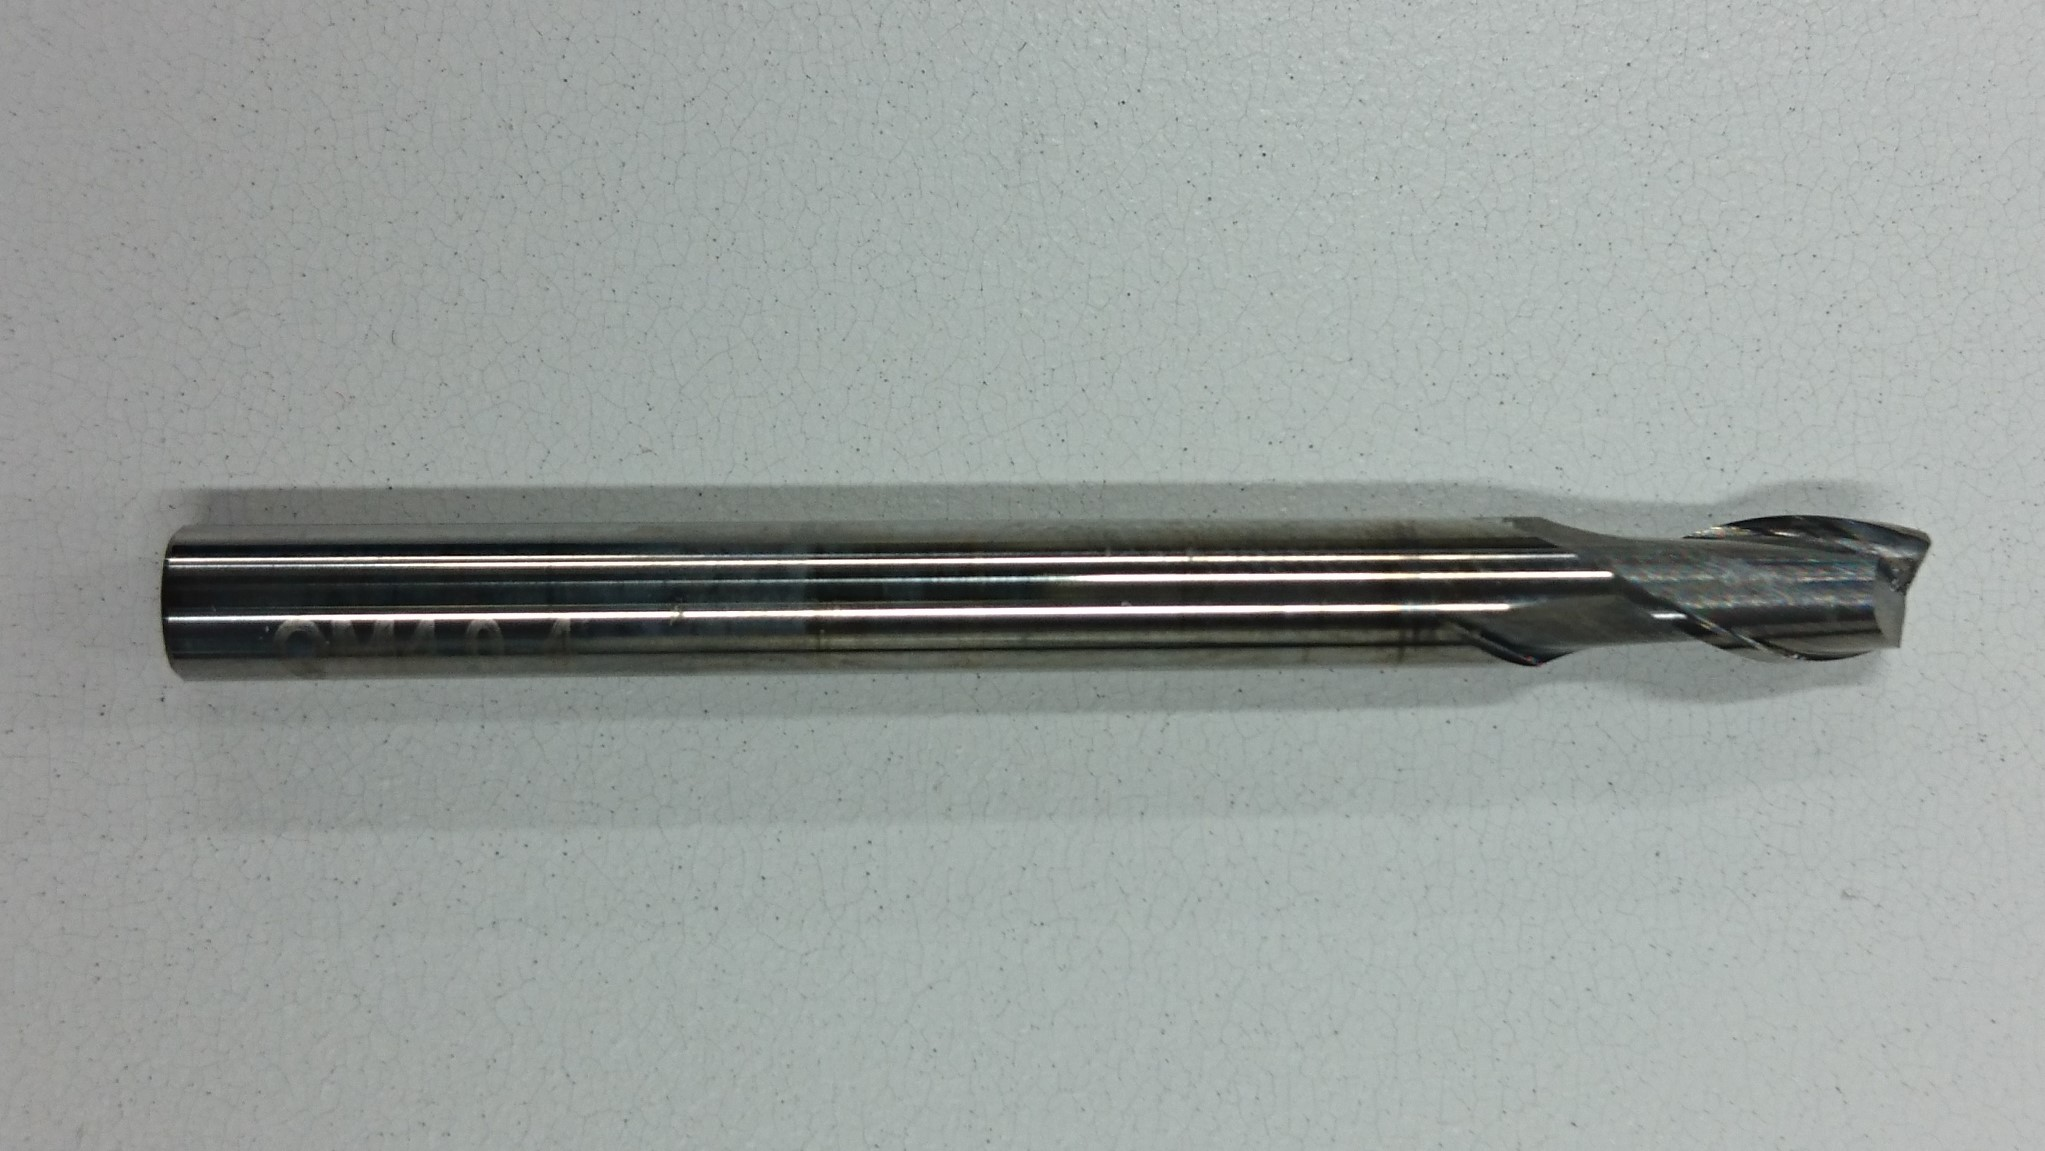
\includegraphics[width=\columnwidth]{endmill.jpg}
      \caption{スクエアエンドミル    \label{endmill1}}
    \end{minipage}
    \hspace{0.05\columnwidth}
    \begin{minipage}{0.4\columnwidth}
      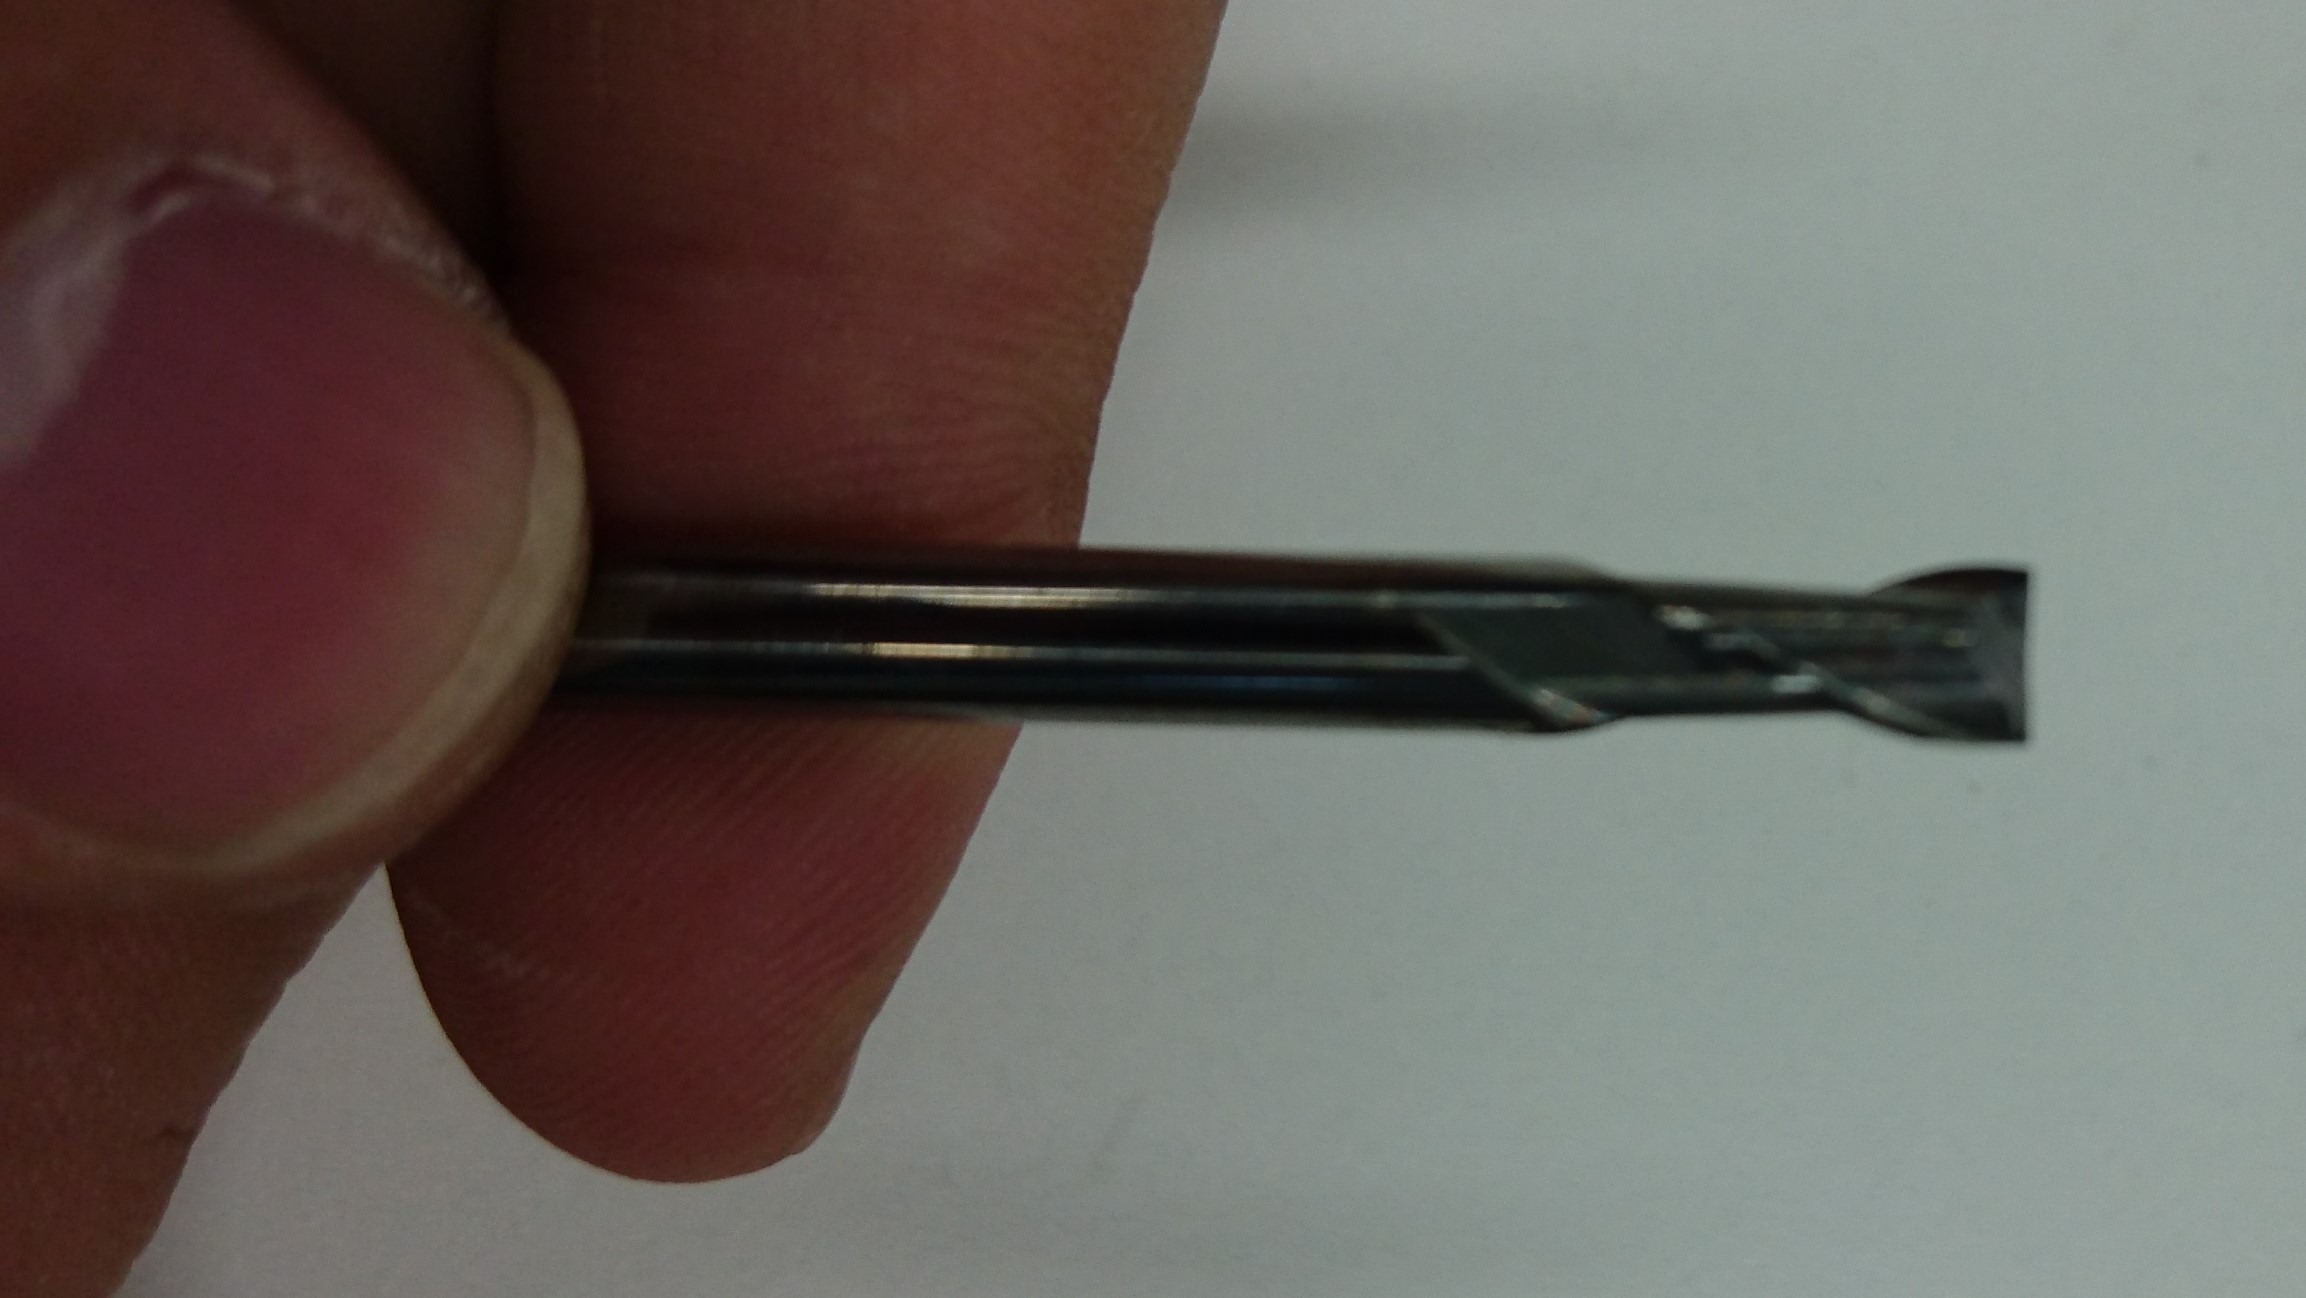
\includegraphics[width=\columnwidth]{endmill_side.jpg}
      \caption{エンドミル刃形    \label{endmill2}}
    \end{minipage}
  \end{center}
\end{figure}

%%画像*2 スクエアエンドミル endmill.jpg endmill_4mm_side.jpg

\begin{figure}[tbh]
  \begin{center}
    \begin{minipage}{0.4\columnwidth}
      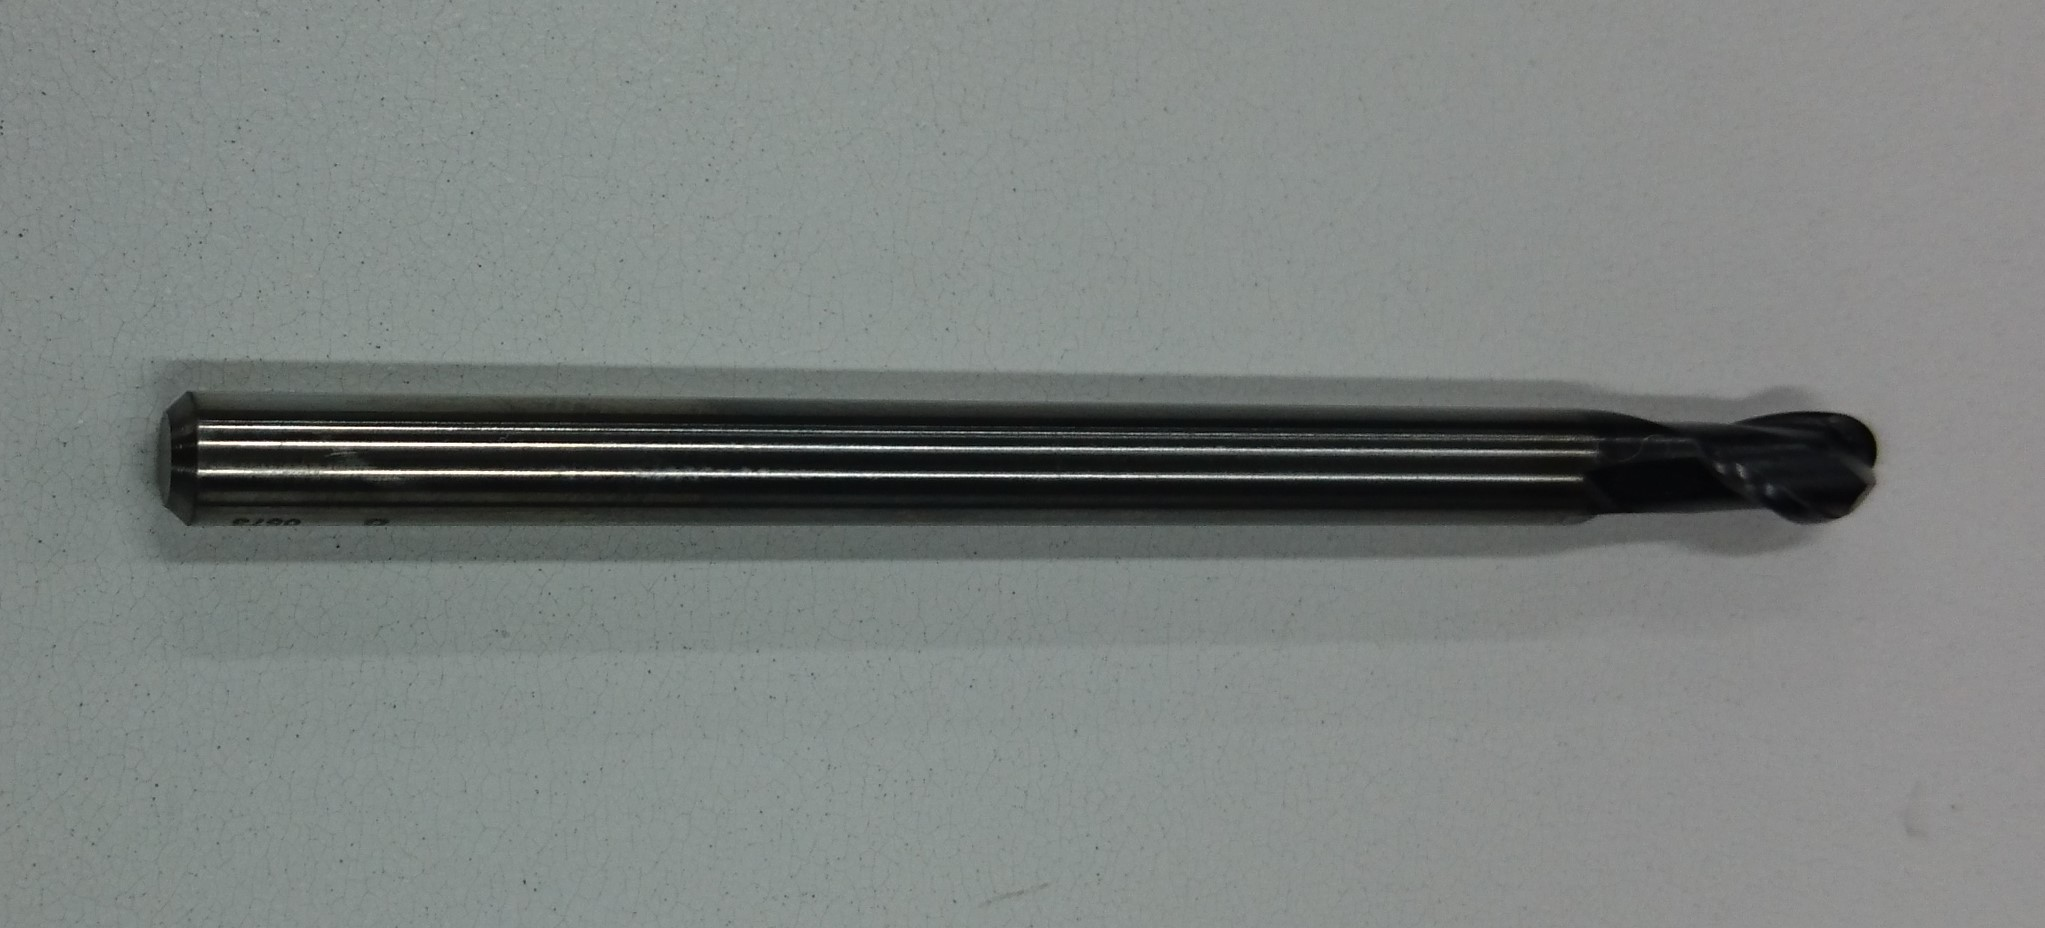
\includegraphics[width=\columnwidth]{bollendmill.jpg}
      \caption{ボールエンドミル    \label{bollendmill1}}
    \end{minipage}
    \hspace{0.05\columnwidth}
    \begin{minipage}{0.4\columnwidth}
      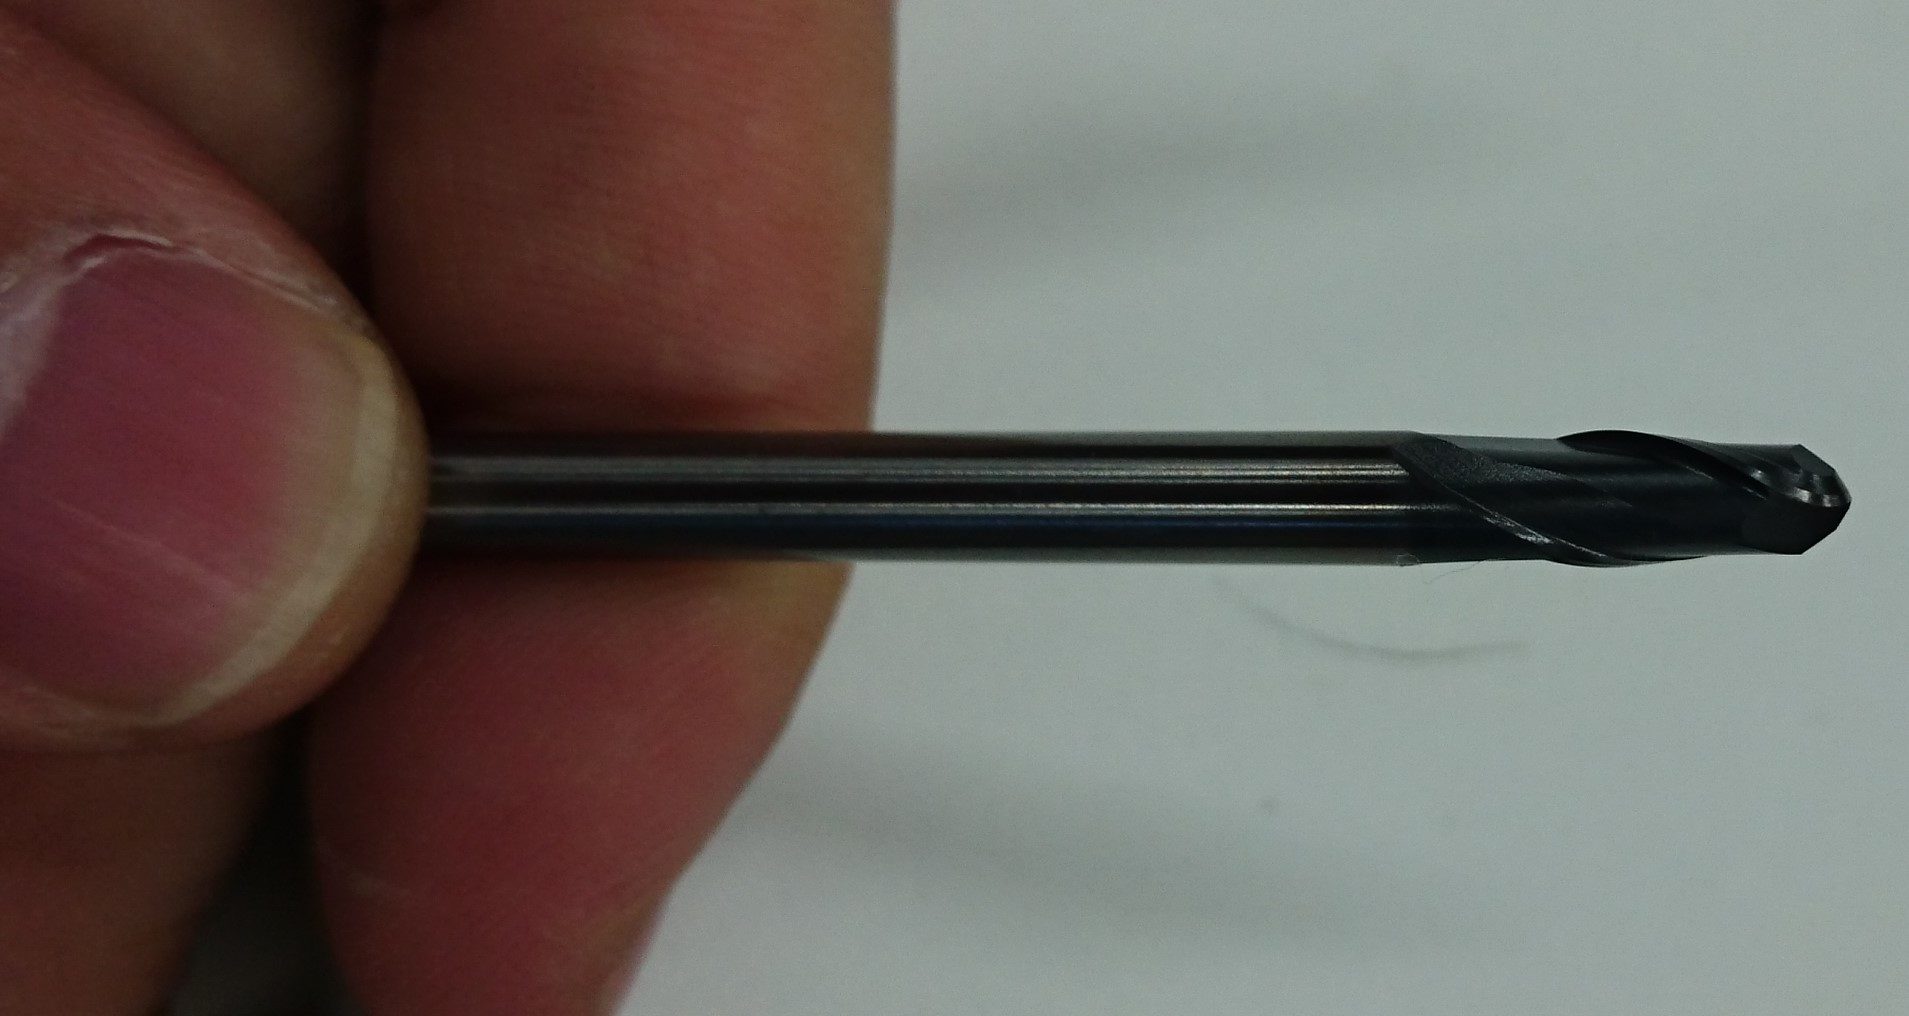
\includegraphics[width=\columnwidth]{bollendmill_side.jpg}
      \caption{エンドミル刃形    \label{bollendmill2}}
    \end{minipage}
  \end{center}
\end{figure}

%%画像*2 ボールエンドミル bollendmill.jpg bollendmill_side.jpg

刃直径とは、エンドミルを回転した時に先端の刃の一番外側が描く円の直径を指します。これによって切削が可能な幅と、回転軸からどの程度の距離の範囲が切削されるかが決まります。例えば刃直径が3mmのエンドミルの場合、エンドミルの中心が通った直線を中心とした、幅3mmの領域が切削されます。また、直径が大きいと切削領域が大きくなるため、基本的に切削時間は短くなります。ポケット加工(後述)など、切削領域が大きく時間がかかる場合は、影響が出ない範囲で大きなエンドミルを使うと加工時間の短縮が図れます。

シャンク径とは、エンドミルのうち刃のついていない上部の円筒状の部分の直径のことであり、写真のエンドミルの場合Φ4となっています。普段よくCNCで使われる程度のサイズだと、4mm,6mm,10mmなどが一般的です

有効刃長とは、エンドミルのうち切削が可能な長さのことで、これと等しい長さだけ深く切削を行えます。例えば、上の写真のエンドミルについては、有効刃長が8mmのため、厚みが8mmまでの板材であれば基本的に問題なく切削が行えます。しかし、それ以上の厚みの板材だと、刃が無いシャンク径が4mmの部分までエンドミルを挿し込むことになり、シャンクと刃の間のテーパー部分が板材に接触して事故の原因になります。有効刃長を超えた切削はCNCの故障の原因になるため、使用の際には十分に注意をしましょう。\\

\subsection{ダウンカットとアップカット}

ダウンカットとアップカットは、被切削材に対しエンドミルの回転方向と切削方向がどのようになっているかを表しています。ダウンカット(下向き削り)とは、工具の刃が未切削の部分に当たって材を削り下げる削り方、アップカット(上向き削り)とは、工具の刃が切削済みの部分に当たって削りあげる削り方を指します。ダウンカットでは切り込み時が最も材への食いこみが大きく次第に小さくなり最終的に0になるのに対し、アップカットでは食い込みが最初は0で次第に大きくなります。詳細は省きますが、びびりや摩擦熱が生じて工具寿命が短くなるなどの理由から、基本的にCNC加工の際はダウンカットで加工を行います。通常、エンドミルの回転方向は正転(上からみて時計周り方向)であるため、外形カットを行う場合、エンドミル自体の経路も時計回りになります。\\

\begin{figure}[tbh]
  \begin{center}
    \begin{minipage}{1.0\columnwidth}
      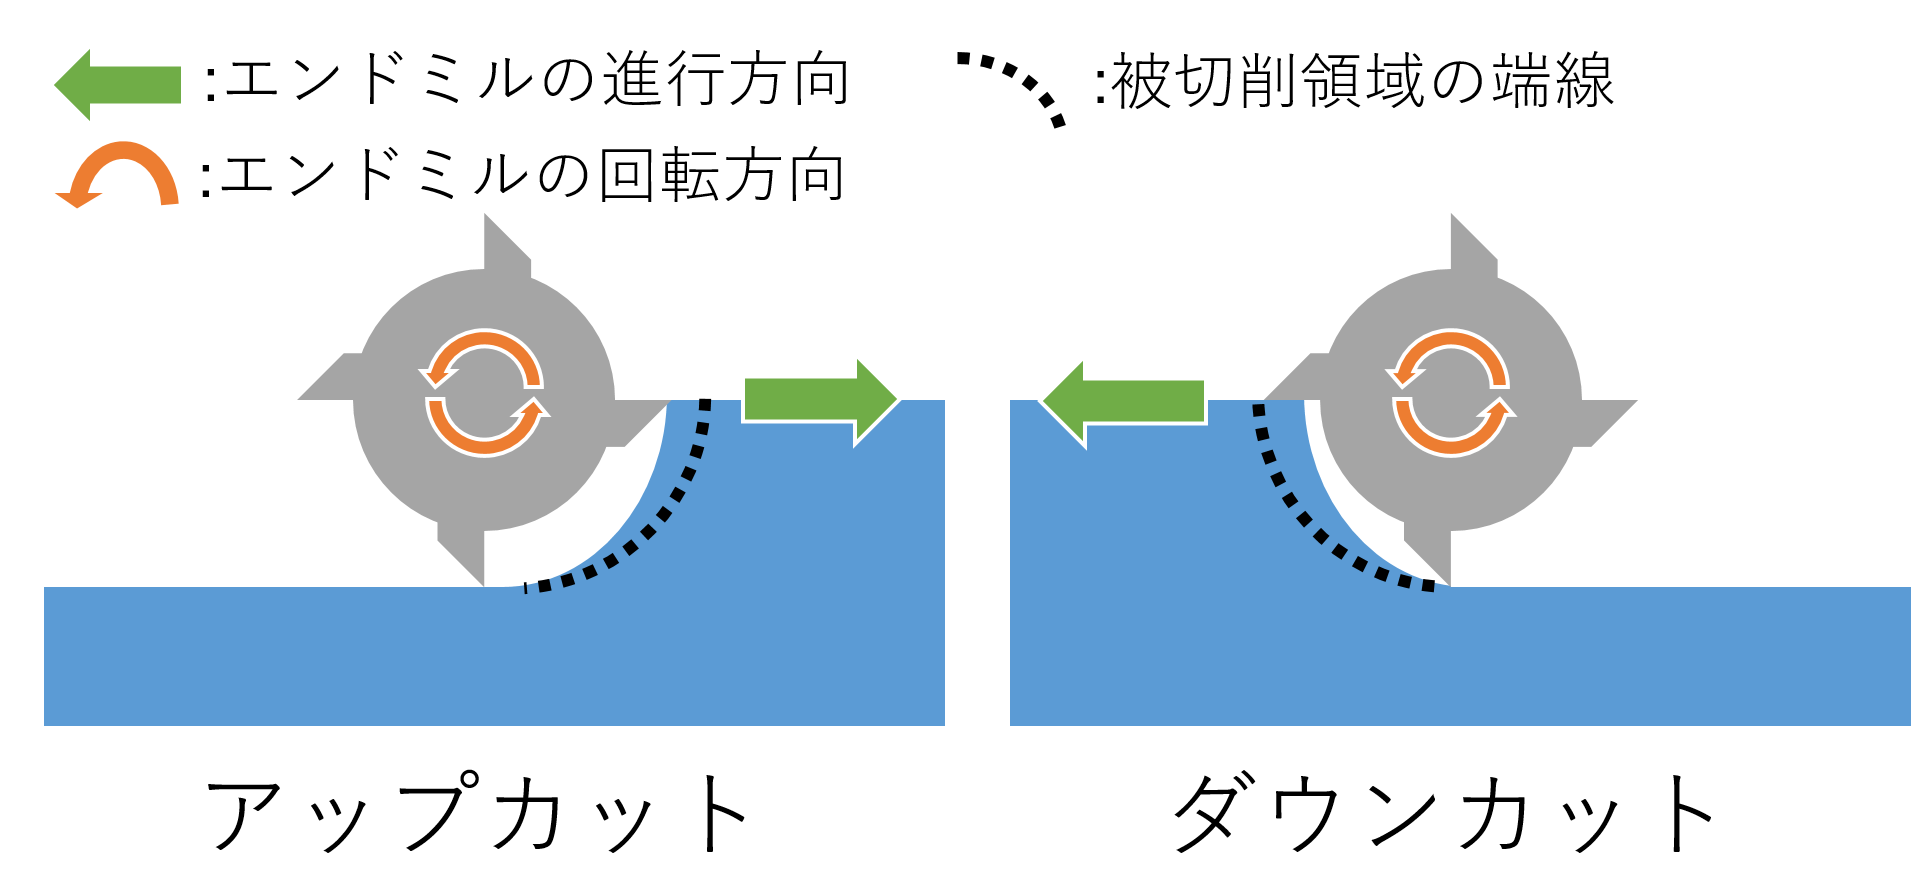
\includegraphics[width=\columnwidth]{cutting.png}
      \caption{ダウンカットとアップカット    \label{cutting}}
    \end{minipage}
  \end{center}
\end{figure}

%%画像*1 ダウンカットとかの図 cutting.png

\subsection{エンドミルの固定方法}

エンドミルの固定方法には、1.いもねじ,2.ドリルチャック,3.コレットの3種類ほどが一般的です。\\
いもネジによる固定は特に書くことはありません。カップリングなどと同様に留めれば大丈夫ですが、六角ねじの穴が死にやすいので過度に力を入れて締めすぎないようにしましょう。\\
ドリルチャックについても、一般的なボール盤のドリルのチャック方式と同じです。チャックハンドルはサイズの合ったものを使いましょう。また、ボール盤でも同様ですが、まれにチャックハンドルを付けたままエンドミルを回してチャックハンドルを吹き飛ばす事故が起きるので、気を付けましょう。当たると痛いです。\\
最後にコレットによる固定です。主にATC付のCNCでエンドミルを使用する際などに使います。スリットの入った紡錘形の金属部品の中心にエンドミルを挿し、周りを締め付けることで固定を行います。面で抑えてくれるため、他の固定方法よりしっかりと固定が可能です。\\
どの固定方法にしても共通で気を付けることとしては、材料の上面にエンドミルがぴったりついた状態で固定し、原点合わせを行うことが挙げられます。エンドミルを材に自重で接触させた上でチャックを行うなどの方法が容易ですが、エンドミルの先端に前回の加工の削りカスや、材の固定用の両面テープの粘着部分などが付いていると、最初の固定の際にエンドミル原点がZ軸上方向にずれるため、削り残しが出てしまうことがあります。加工のたびにエンドミルをパーツクリーナーなどできれいにしましょう。\\

\clearpage
\section{材料の基本}

材料としてよく用いられるものとして、樹脂と金属があります。それぞれについて、具体的な種類を含めて解説します。\\

\subsection{樹脂}

主に用いられる樹脂材として、アクリル樹脂,ABS,POM,ポリカーボネート,MCナイロンなどが挙げられます。特徴としては、金属と比べて切削加工が容易であることと、柔軟性が高いことが挙げられます。厚み方向が厳密ではない場合があることに注意が必要で、例えばt5で売られている板の実寸の厚みがt5.7だったりします。ここではそれぞれの特徴について記述します。物性のまとめは表\ref{plastic_table}を参照してください。\cite{pla_properties}\\

\subsubsection{アクリル樹脂}

樹脂板の中でも安価で、透明で見た目が綺麗なこと、レーザー加工が綺麗に行えること、アクリル用接着剤で溶着が容易なことが利点です。ただし衝撃に弱く、割れる時にはパキっと割れるので、ギヤなど機械的強度が必要な場合にはお勧めしません。\\
\subsubsection{ABS}

アクリルの次に安価で、アクリルより機械的強度が高いです。樹脂の中でも融点が低めで、融けてエンドミルにへばりつきやすいので、加工する速度に注意が必要です。レーザー加工も可能ですが、切断面がアクリルより粗くなりがちです。また、融点が低いことから3Dプリンタのフィラメントに良く使われます。\\
\subsubsection{ポリカーボネート}

POMよりも機械的強度が高く粘り強いため、衝撃があってもそうそう割れないという特徴があります。加えて、アクリル用接着剤での溶着も容易となっています。加工性はABSやPOMなどより劣るため、注意が必要です。また、加工の際に除去しにくいバリが残るという点もあります。見た目がアクリルと近いのですが、異なる特徴として弾性がアクリルより強いことと、断面が少し青みがかっていることがあげられます。\\
\subsubsection{POM}

滑りが良いので、摺動部などに向いています。レーザー加工も可能で、アクリルの次に綺麗に切れます。バネ質で機械的強度も高めで、色々と手ごろでちょうどよいため、使いやすい素材です。撃力で割れることもあるので過信は禁物です。\\
\subsubsection{6ナイロン}

MCナイロンとも呼ばれる、既製品の樹脂ギヤにも用いられる樹脂材です。機械的強度はこの中では最も高いですが、ポリカーボネートと同様にバリが除去しにくいことと、価格が高価なことが良くない点として挙げ られます。また、吸湿して膨張するという特徴もあるため、例えば長い梁のようなパーツを作ると、湿気を吸ってものすごくたわむので注意が必要です。\\
\subsection{金属}

金属を用いる理由としては、一番に重量当たりの強度で樹脂より優れていることがあげられます。\\
\subsubsection{アルミ合金}

アルミ合金と一口に言っても、、色々と種類があります。筆者がよく使っていたのはA5052(板材)やA6063(角パイプ)などです。型番と種類の対応は表\ref{alminium_num_table}のようになります。ここでは、A5052,A2017(ジュラルミン),A2024(超ジュラルミン),A7075(超々ジュラルミン)を紹介しますが、CNC加工では基本的にA5052を用います。たわみなどが心配な場合は、CADに付属しているCAEで計算した上で、必要なヤング率を満たすものを使用しましょう。ちなみに、ヤング率で比較を行うと、超ジュラルミン>ジュラルミン>超々ジュラルミン>ジュラルミン>工作用アルミとなります。(表\ref{alminium_young_table})特にこだわりがなければ、基本的に工作用のA5052が入手しやすそうです。厚みについては、ぴったり寸法の通りであることが多いようです(購入している業者によるのかは筆者のリサーチ不足です)。通常のCNC加工ではA5052を使うのが良いでしょう。\cite{alminium_properties}\\
%%アルミ:http://www.alumitech.co.jp/html/download5.html
\subsubsection{真鍮}

真鍮の中でもよく用いられるのがC3604(快削真鍮)です。入手性が良く、比重が高い金属の中では加工性が良いため、フライホイールや重りなどの重量物を作る際に向いています。後は、樹脂材との滑りが比較的良いため、溝カムなどの摺動部に用いることもあります。\\
\subsubsection{鉄(ステンレス含む)}

入手が容易な金属の中でも加工が比較的難しく、加えて重いので、荷重が大きくかかる軸など、ロボコン用途では一部の機械的強度が重要なパーツを除いてあまり多くは使われない印象です。CNCでも加工できないことはないですが、長い時間と大量の切削油とエンドミルの犠牲が必要なため、お勧めしません。加工したい場合には強いフライス盤などを使いましょう。\\
\subsection{その他}

樹脂でも金属でもない材料をその他とします。木材などが含まれます。\\
\subsubsection{MDFボード}

Midium Density Fiber Boardの略で、中密度繊維板とも呼ばれるもので、木の繊維を樹脂で板状に固めて作られています。基本的にレーザーで加工を行う材料であり、筆者はt4のものを頻繁に使います。加工が容易な上に木工用ボンドで接着が容易なため、さっとプロトタイピングを行うときには非常に便利です。切削での加工も可能ですが、加工時間などの観点からレーザーで加工されがちです。また、強度は樹脂や金属より当然劣り、また材質が木材に近いことから、柔らかくへこみなども生じやすいため、そもそも厳密な寸法が必要な部品の作成には不向きです。\\

\clearpage
\begin{table}[htb]
  \begin{center}
    \begin{tabular}{|l|c|c|c|c|c|c|} \hline
      樹脂 & 融点 & レーザー加工 & バリの除去性  & 価格(1枚) & ヤング率(MPa) & 比重(g/cm\verb|^|3)\\ \hline
      アクリル        & & o & △  約&¥ 590   &65-77  & 1.19 \\ \hline
      ABS             & & o & o  &約¥790  & 35-59  & 1.05\\ \hline
      ポリカーボネート& & x & △  約&¥ 890   &64-69  & 1.2 \\ \hline
      POM             & & o & o  &約¥1230 & 61-69  & 1.41\\ \hline
      6ナイロン       & & x & △  約&¥ 1710  &41-166  &1.13 \\ \hline
    \end{tabular}
    \caption{樹脂の種類と性質    \label{plastic_table}}
  \end{center}
\end{table}

\begin{table}[htb]
a  \begin{center}
    \begin{tabular}{|l|l|l|} \hline
      型番 & 種類 & 具体例 \\ \hline
      1000番台& 純アルミ &  \\ \hline
      2000番台& Al-Cu系 & ジュラルミン,超ジュラ \\ \hline
      3000番台& Al-Mn系 &  \\ \hline
      4000番台& Al-Si系 &  \\ \hline
      5000番台& Al-Mg系 & 工作用アルミ材 \\ \hline
      6000番台& Al-Mg-Si系 &  \\ \hline
      7000番台& Al-Zn-Mg系 & 超々ジュラルミン \\ \hline
    \end{tabular}
    \caption{アルミの型番と種類,具体例    \label{alminium_num_table}}
  \end{center}
\end{table}

\begin{table}[htb]
  \begin{center}
    \begin{tabular}{|l|l|l|} \hline
      種類 & ヤング率(GPa) & 比重(g/cm\verb|^|3) \\ \hline
      A5052(工作用アルミ)& 70.6 & 2.79 \\ \hline
      A6063(角パイプ)& 68.6 & 2.70 \\ \hline
      A2017(ジュラルミン)& 72.6 & 2.75 \\ \hline
      A2024(超ジュラルミン)& 73.5 & 2.78 \\ \hline
      A7075(超々ジュラルミン)& 71.6 & 2.81 \\ \hline
    \end{tabular}
    \caption{アルミの種類とヤング率,比重    \label{alminium_young_table}}
  \end{center}
\end{table}



\chapter{実践編}
ここからを実践編とします。具体的には、\\\\
  工程1.CADソフト(inventor)での部品設計\\
  工程2.CAMソフト(Cut2D)でのツールパス設計\\
  工程3.CNC(RD300,USBCNC)での作業、清掃\\\\
  という順番で切削部品の製作を行います。
  まず工程1では、CADによる部品の設計と、経路設計に必要な外形線を含むvector形式ファイルの作成を行います。この工程では、製作する部品の二次元情報からvector形式ファイルを作ります。次に工程2では、工程1で作成したvector形式ファイルを元にして、実際に加工を行う経路を設計し、NCデータの作成を行います。この工程で、vector形式ファイルの調整と、切削を行う深さ情報を加えた三次元のツールパスの設計を行います。最後に工程3では、工程2で設計したNCファイルをUSBCNCで読み込み、実際の切削を行います。\\

\clearpage
\section{工程1.CADソフト(inventor)での部品設計}
今回はinventorを使って設計を行います。学生であれば学生用のライセンスがオンラインからすぐに使え、ドキュメントも充実しているのが良い点です。\\

\subsection{基本的な部品設計}
CNCで加工が可能な部品の形状には限りがあり、基本的に底面に平行な平面またはと底面に垂直な側面の集合のみを持つ立体である必要があります。基本的には板材から切り出せる形状のパーツであれば加工で製作することが加能です。曲面を含む三次元的な部品の場合も、前述のボールエンドミルを使えば加工は可能ですが、ここでは簡単のため説明しません。今回の実践編では、図\ref{parts_dft}のようなパーツを加工します。\\

\begin{figure}[tbh]
  \begin{center}
    \begin{minipage}{0.9\columnwidth}
      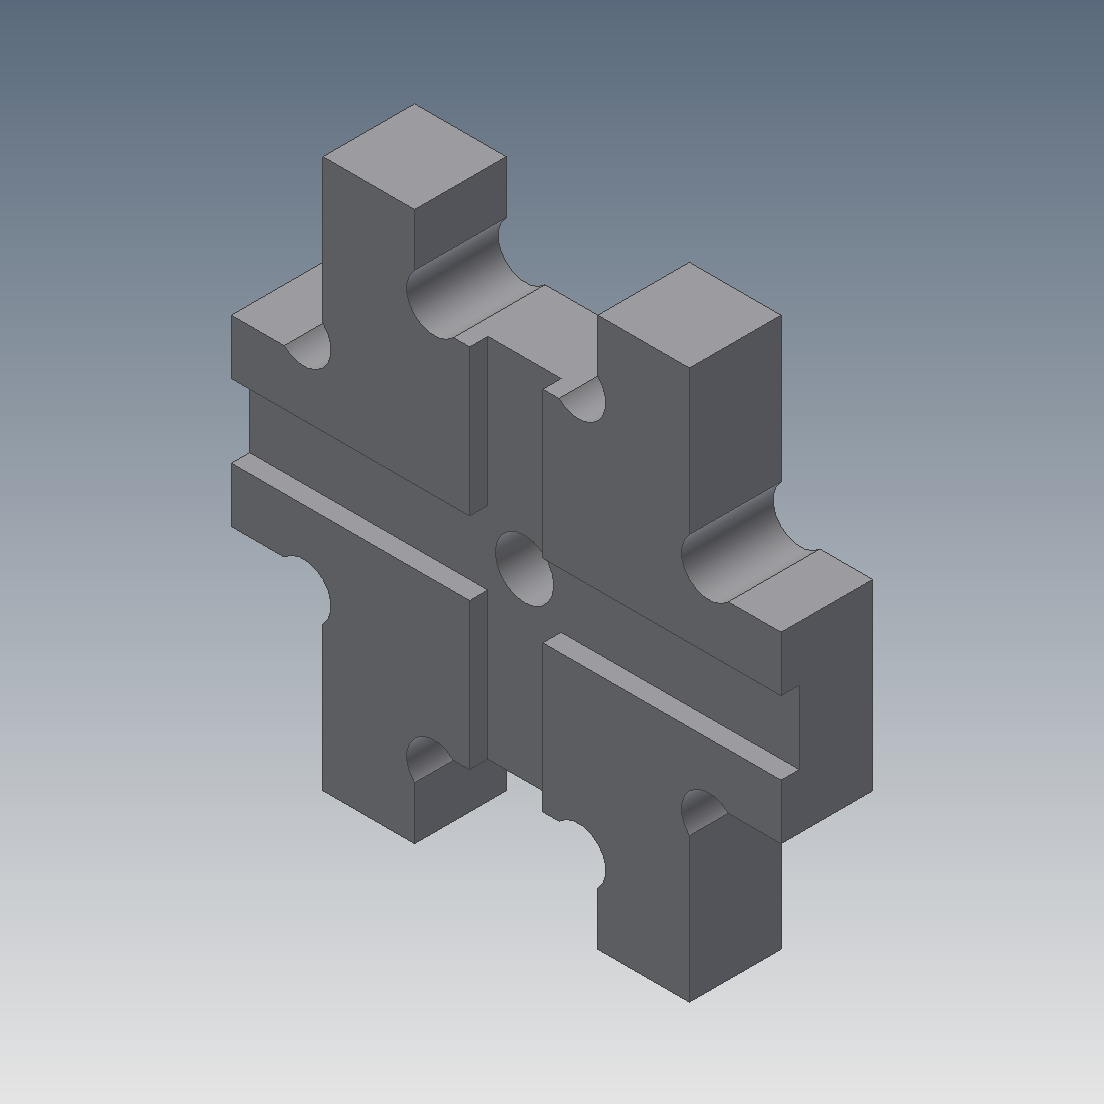
\includegraphics[width=\columnwidth]{piece_1_hoge.png}
      \caption{今回作る部品    \label{parts}}
    \end{minipage}
  \end{center}
\end{figure}

%%画像*2 部品の例のCAD図 piece_1_hoge.png piece_1_dft2.png

\subsection{部品設計で気を付けること}
CNCで切削加工を行う部品を設計する上で、エンドミルによる加工を理解する必要があります。具体的には、切削される領域は円が移動した領域であることに注意しなければいけません。例えば、図\ref{no_kirinuki}の設計では、外形の周囲をそのまま削ると、角の部分の内側に削り残しが生じます。はめ込みを行うパーツなどの場合、その削り残し部分が干渉する場合があります。そのため、図\ref{kirinuki}のように、円形の切り抜きをあらかじめ設計に追加しておくことで、角の部分をすべて削りきることができます。また、外形の線に沿ってエンドミルが動くという性質から、エンドミルの直径と同じ径の穴をあけることは基本的にできません。この問題の解決方法としては、穴径をエンドミル径より微妙に大きくするなどが挙げられ、工程2で詳細を書きます。また、当然ですがCNCで加工が可能な領域より大きな部品を作ることはできません。今回説明に使うRD300というCNCでは、加工領域が220mm*300mmであるため、加工できるのはそのサイズまでということになります。\\

\begin{figure}[tbh]
  \begin{center}
    \begin{minipage}{0.4\columnwidth}
      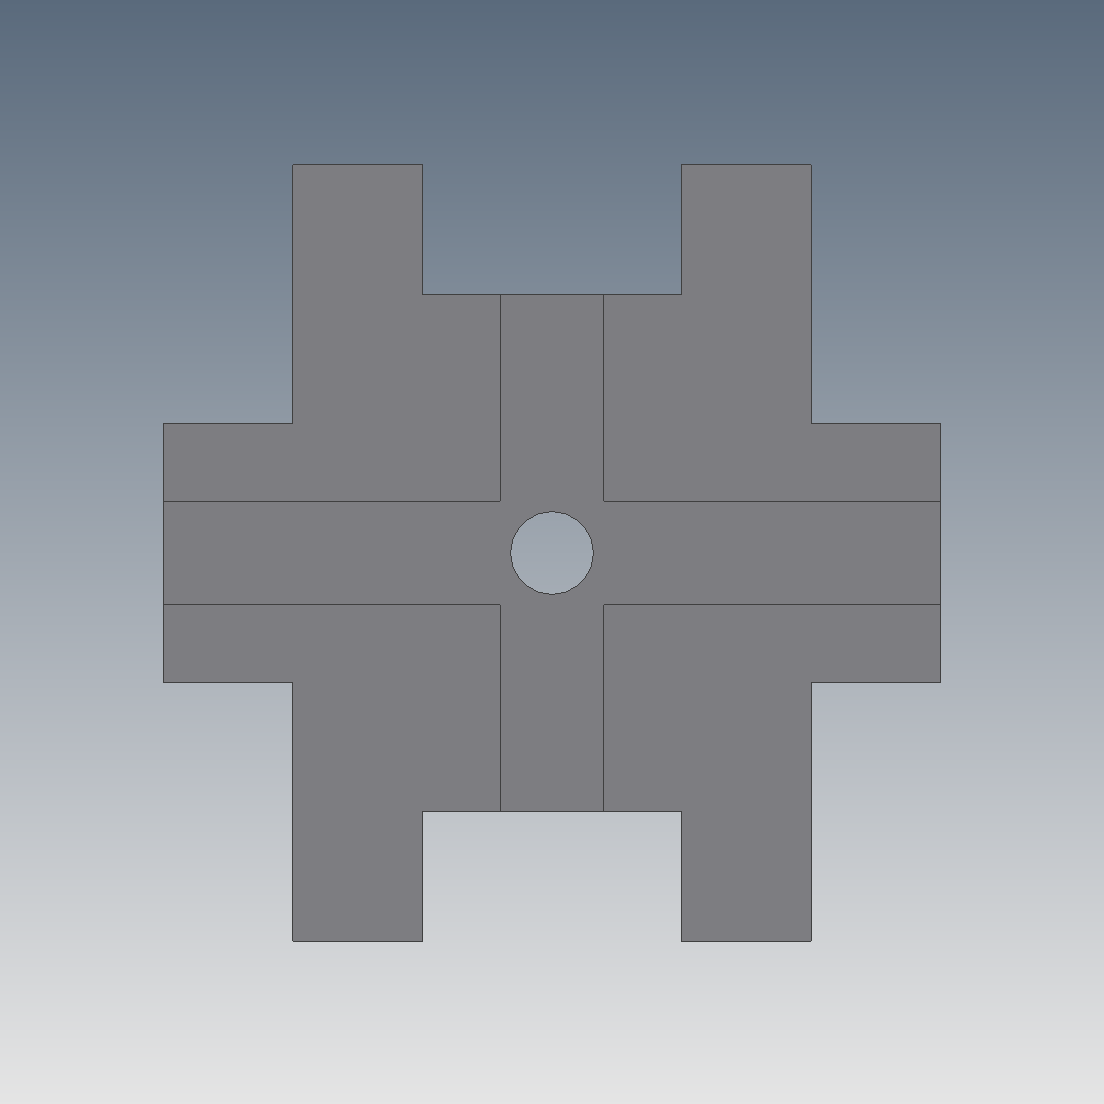
\includegraphics[width=\columnwidth]{piece_1_ue5.png}
    \end{minipage}
    \hspace{0.05\columnwidth}
    \begin{minipage}{0.4\columnwidth}
      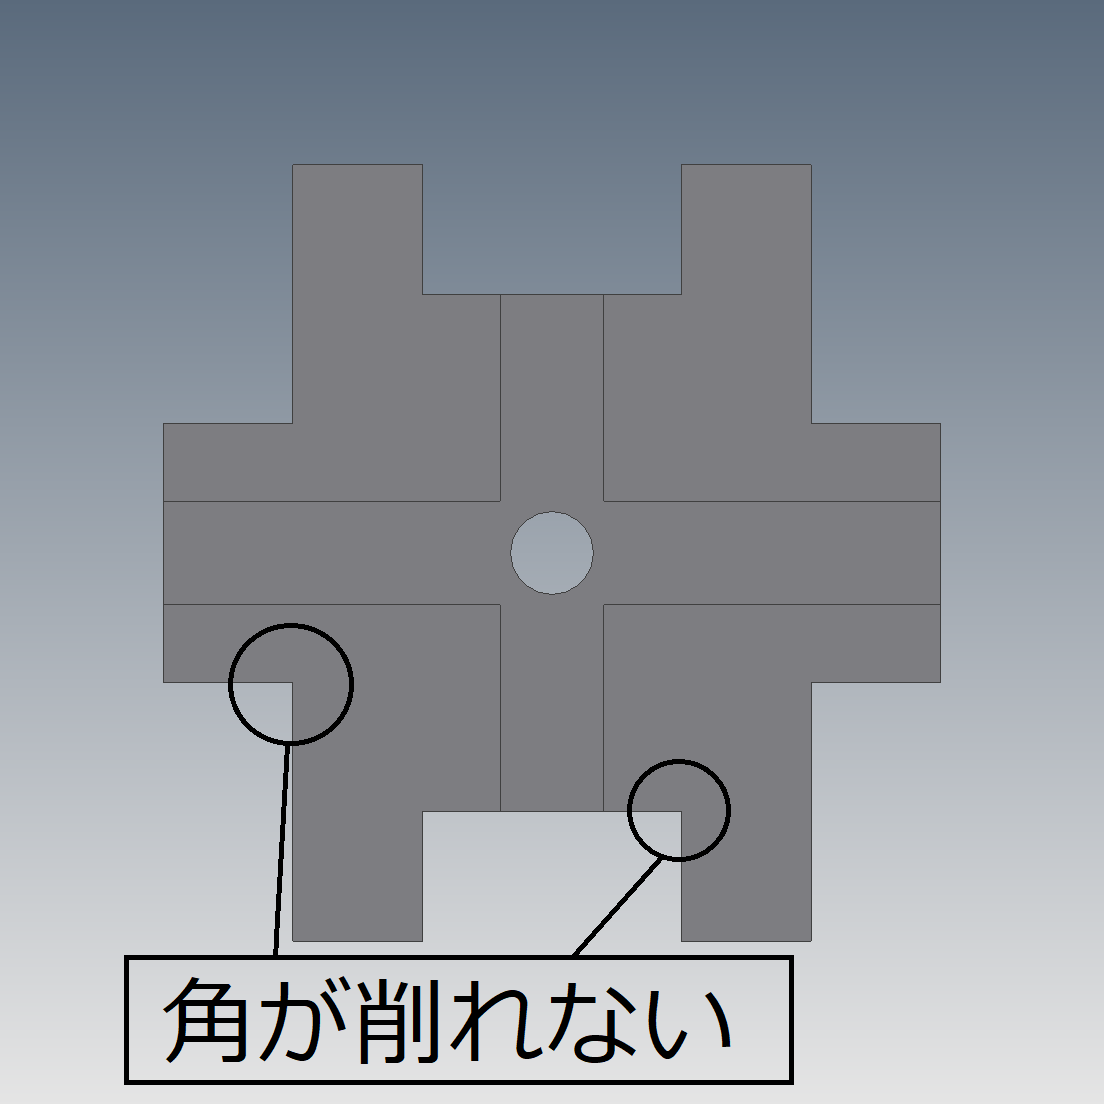
\includegraphics[width=\columnwidth]{piece_1_ue4.png}
    \end{minipage}
    \caption{切り抜きなし    \label{no_kirinuki}}
  \end{center}
\end{figure}

%%画像*2 部品の例のCAD図(ダメな方) piece_1_ue5.png piece_1_ue4.png

\begin{figure}[tbh]
  \begin{center}
    \begin{minipage}{0.4\columnwidth}
      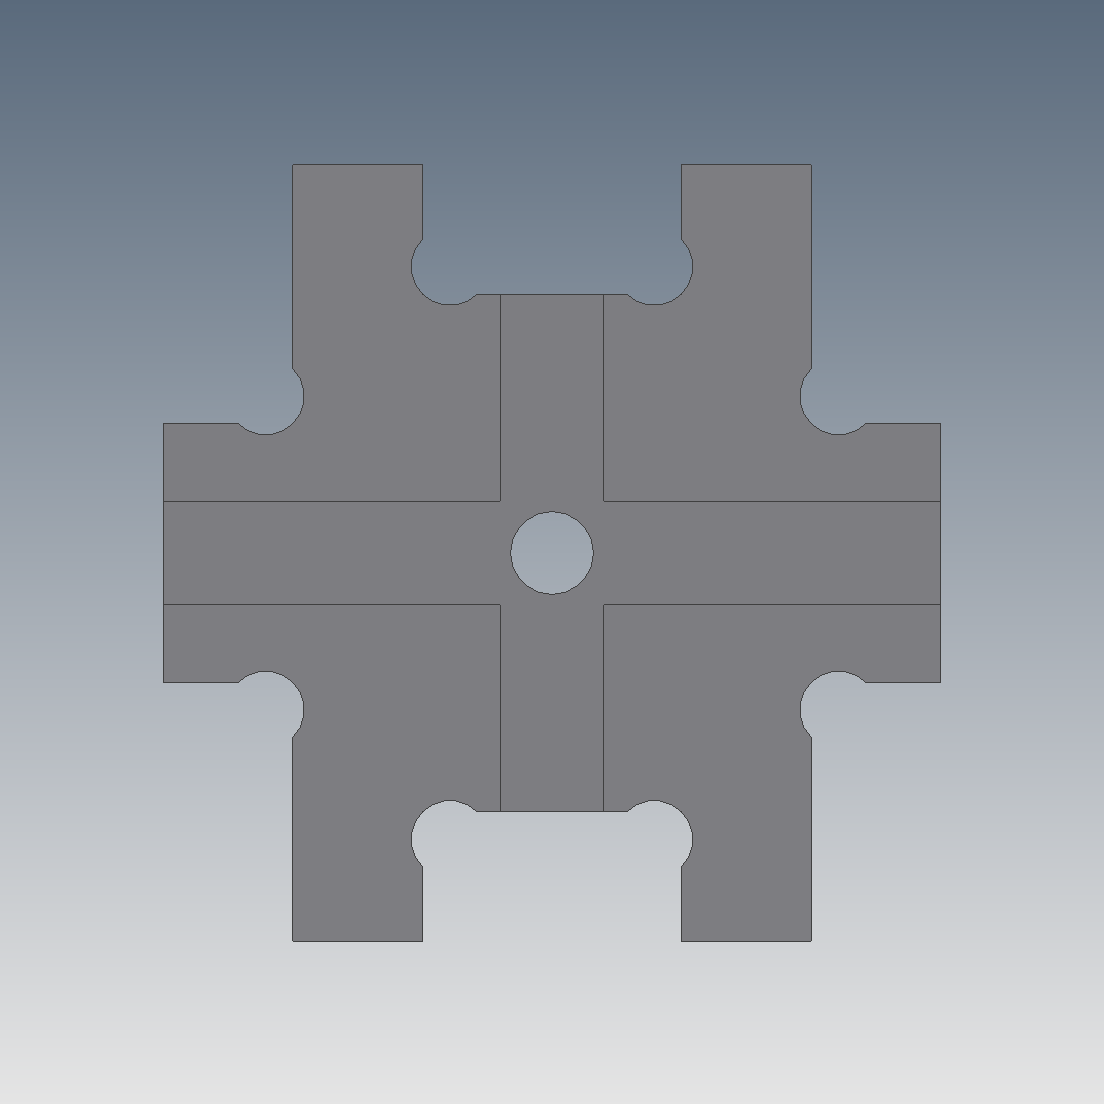
\includegraphics[width=\columnwidth]{piece_1_ue3.png}
    \end{minipage}
    \hspace{0.05\columnwidth}
    \begin{minipage}{0.4\columnwidth}
      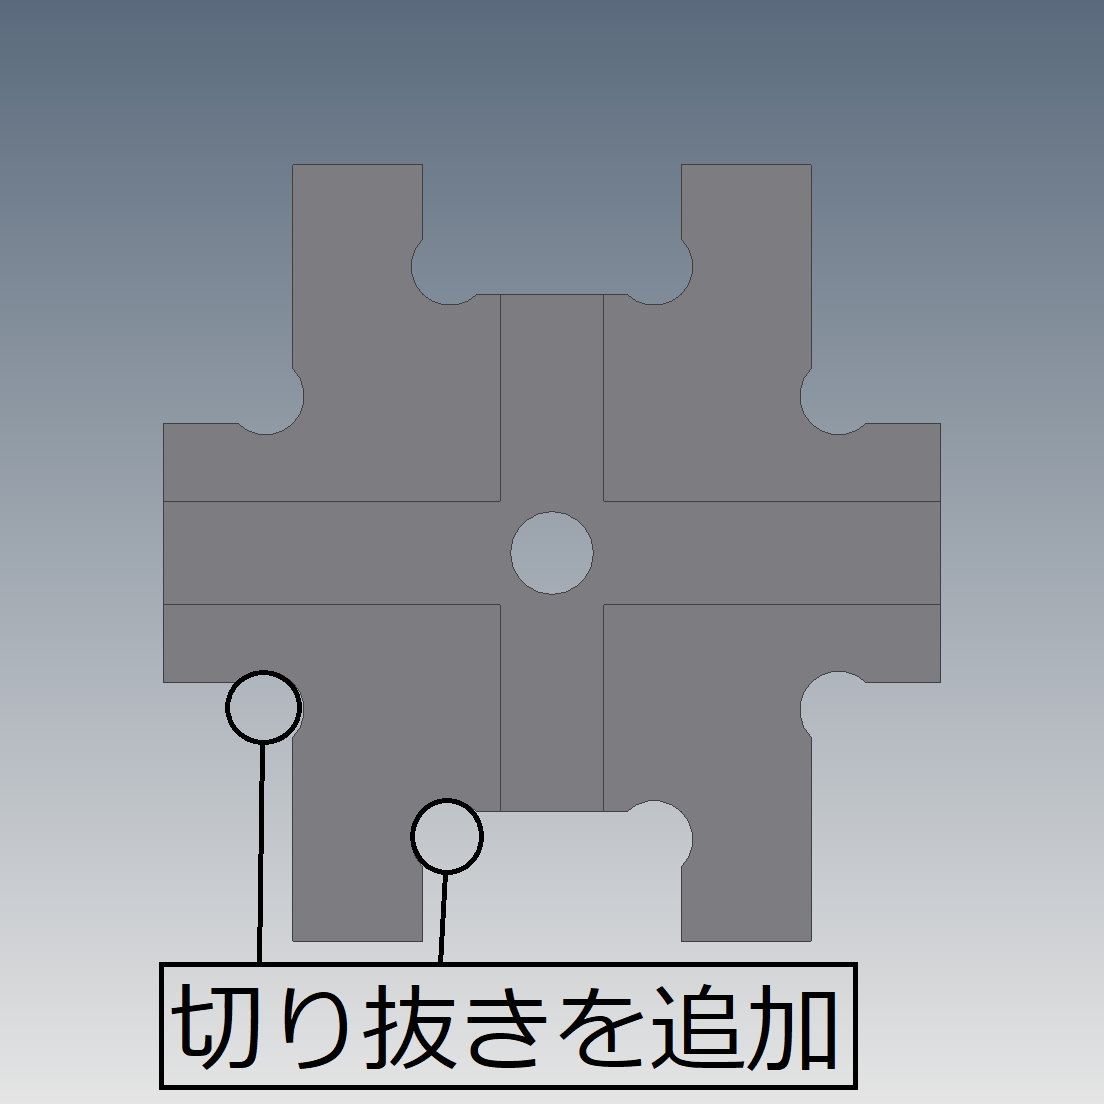
\includegraphics[width=\columnwidth]{piece_1_ue6.png}
    \end{minipage}
    \caption{切り抜きあり    \label{kirinuki}}
  \end{center}
\end{figure}

%%画像*2 切り抜く部分と切り抜いた後の画像 piece_1_ue3.png piece_1_ue6.png
\clearpage
\begin{figure}[tbh]
  \begin{center}
    \begin{minipage}{2.0\columnwidth}
      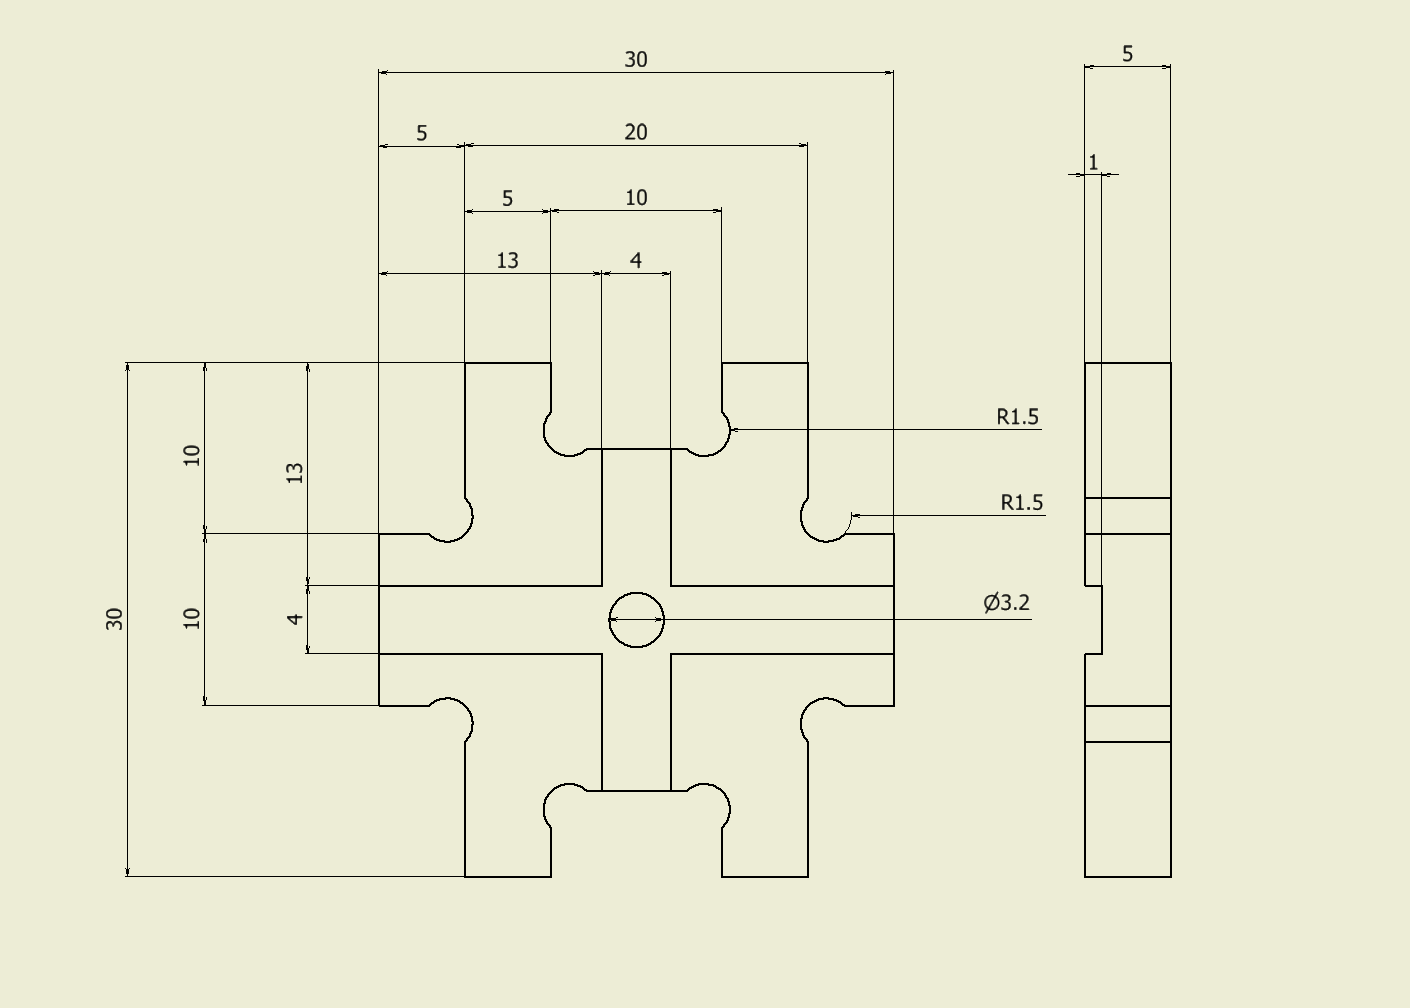
\includegraphics[width=\columnwidth]{piece_1_dft2.png}
      \caption{部品の図面    \label{parts_dft}}
    \end{minipage}
  \end{center}
\end{figure}


\clearpage
\begin{onecolumn}
\subsection{vector形式ファイルの作成}
inventorでの部品作成が終わったら、CADの図面作成機能を用いて、vector形式のファイルを作成します。Cut2Dで読み込めるvector形式ファイルにはdxf,pdf形式などがありますが、ここではpdfを用います。vector形式ファイル作成の際に気をつけることとしては、\\
  1.縮尺を1:1にする\\
  2.図面中の部品名や図表などを削除する\\
  3.図面中に隠線を表示しない\\
  などが挙げられます。縮尺を1:1にするのは部品のサイズを設計した通りに加工するため、図面中の図面枠・隠線を消すのはCut2Dで経路を作る時に余計な線をなるべく残さないため行います。図表や隠線については、削除するのを忘れた場合であっても、この後の工程で修正が可能ですが、面倒なのでなるべく残さないようにしてください。\\
inventorで図面を作る場合の手順として、まず左上のプルダウンメニューから図面の新規作成を行います。次に図\ref{no_jis}と図\ref{cutting_image}を参考にして、デフォルトの図面枠とJIS表記を削除して部品の図面を張り付けます。その際に図\ref{window}の画面で図面設定を行えるので、縮尺・隠線・図面の方向を決めてOKを押します。ここまで終わったら、図\ref{pdf_save}を参考にして図面をpdf形式で保存を行ってください。保存できる形式はCADによって異なるのですが、Cut2Dで読み込むことのできる形式で保存を行って下さい(.pdfや.dxfなどが可能)。この工程で、加工したい部品のvector形式のファイルを作成することができました。
\begin{figure*}[tbh]
  \begin{center}
    \begin{minipage}{1.0\columnwidth}
      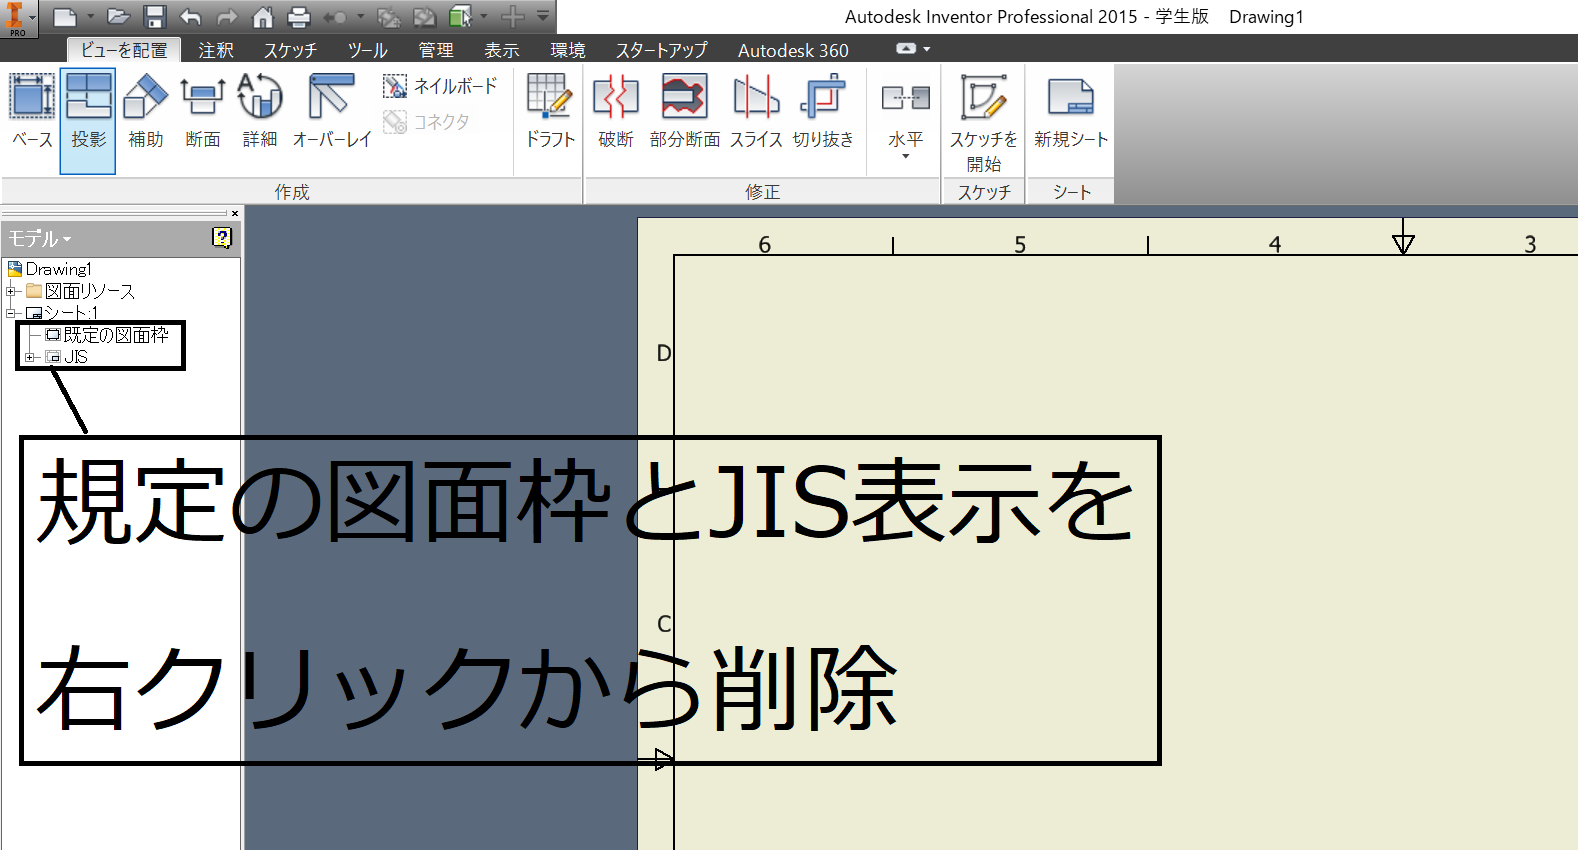
\includegraphics[width=\columnwidth]{plane_trim.png}
    \end{minipage}
    \caption{図面枠・JIS表記の削除    \label{no_jis}}
  \end{center}
\end{figure*}

\begin{figure*}[tbh]
  \begin{center}
    \begin{minipage}{0.8\columnwidth}
      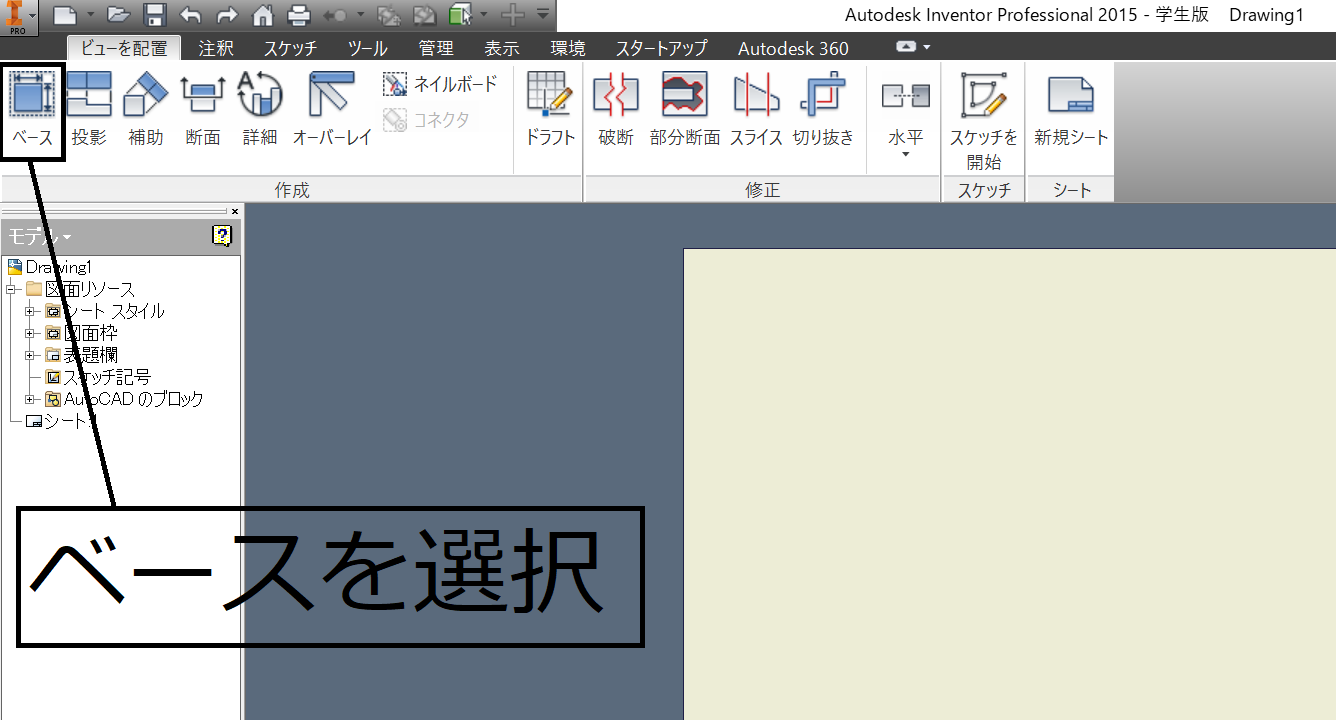
\includegraphics[width=\columnwidth]{no_jis_trim.png}
    \end{minipage}
    \caption{図面の貼り付け    \label{cutting_image}}
    \begin{minipage}{0.8\columnwidth}
      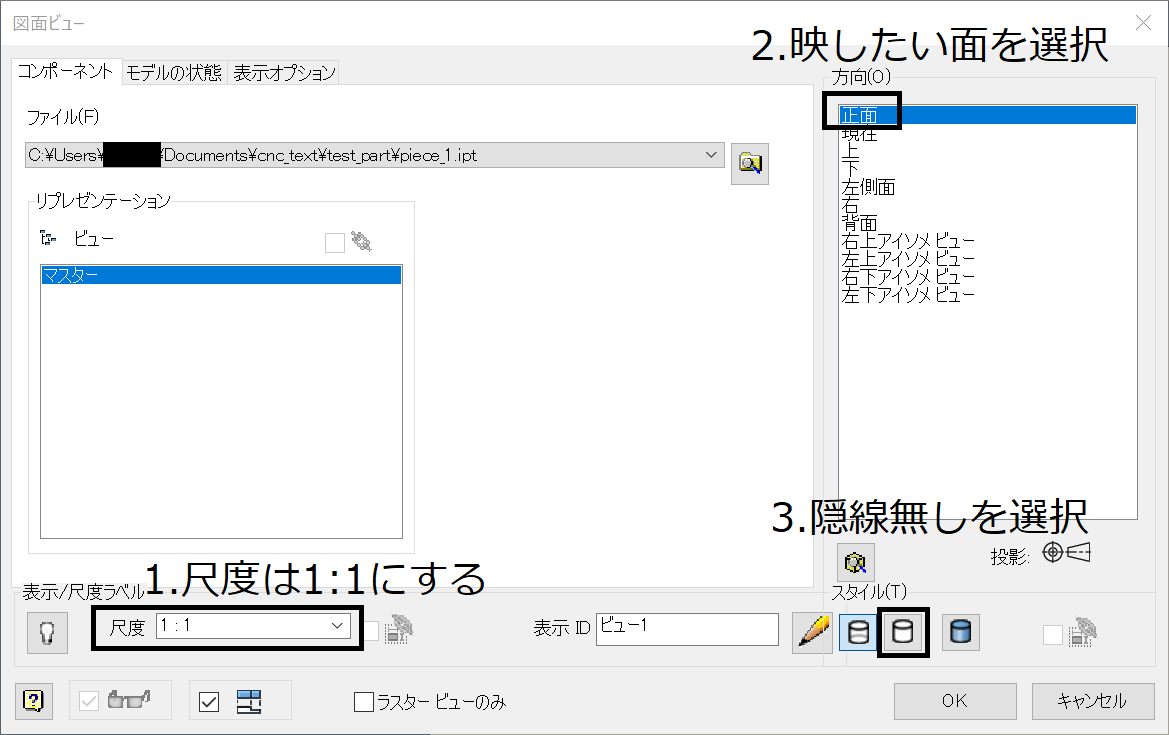
\includegraphics[width=\columnwidth]{window2.png}
    \end{minipage}
    \caption{図面設定    \label{window}}
    \begin{minipage}{0.8\columnwidth}
      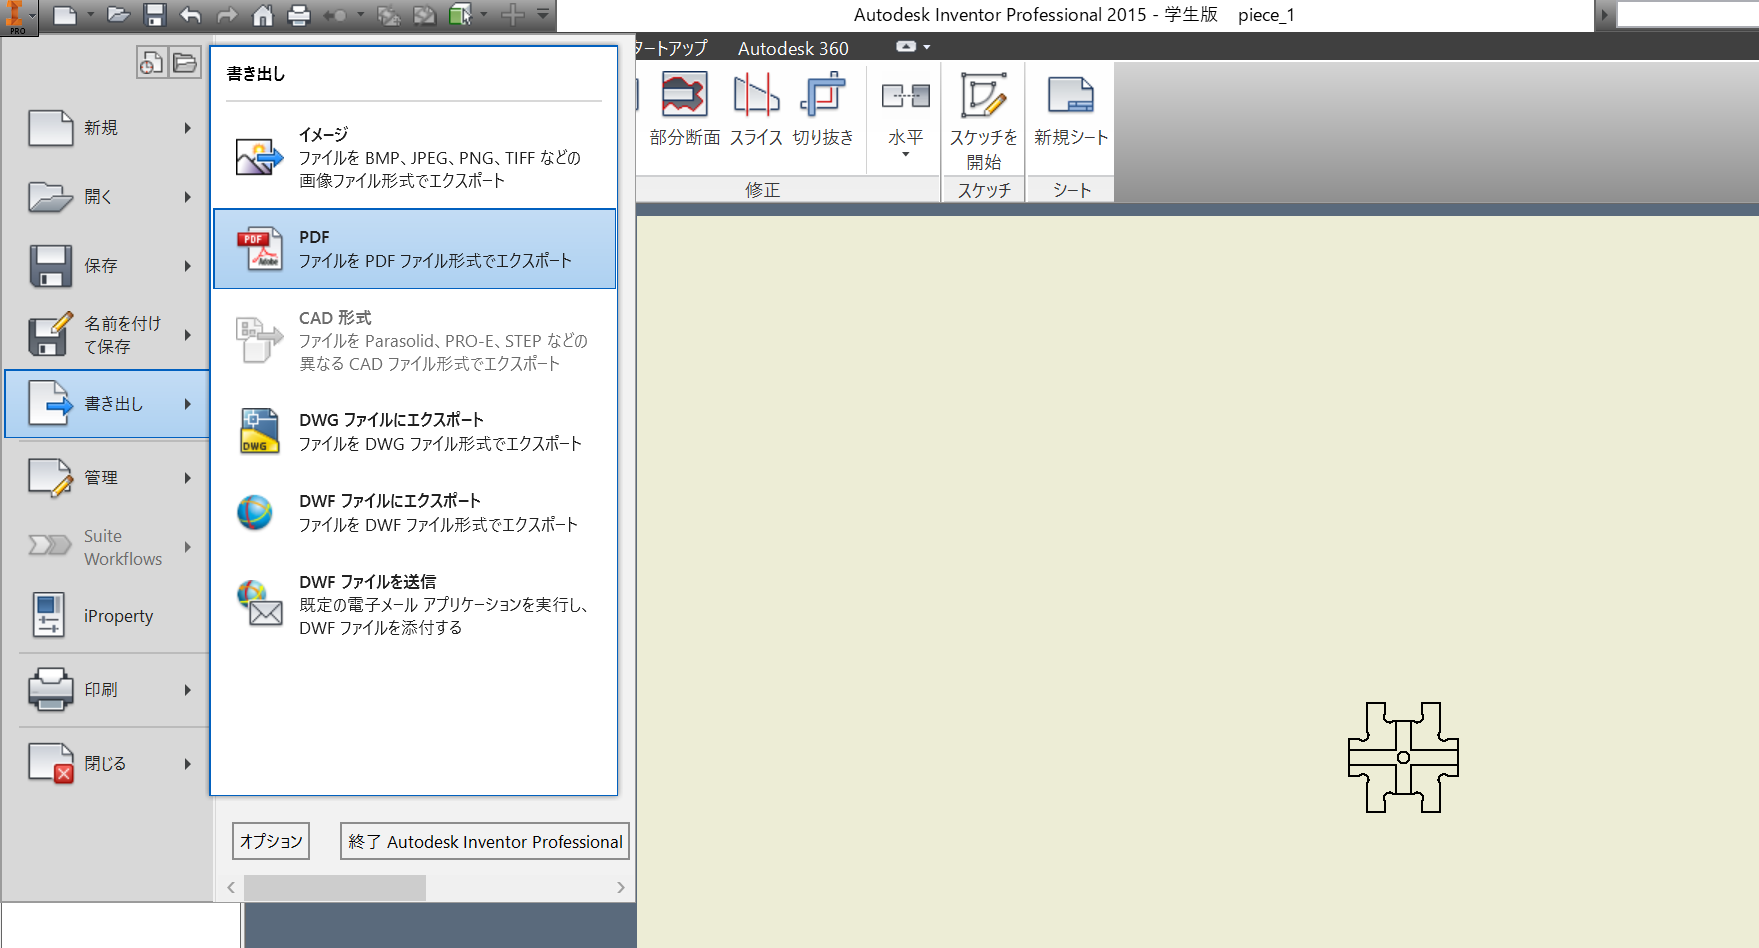
\includegraphics[width=\columnwidth]{hozon2_trim.png}
    \end{minipage}
    \caption{図面の保存    \label{pdf_save}}
  \end{center}
\end{figure*}
\end{onecolumn}

%%画像*4 vector形式保存の仕方 plane_trim.png no_jis_trim.png window2.png hozon2_trim.png


\clearpage
\section{工程2.CAMソフト(Cut2D)でのツールパス設計}
ここではCut2Dでの作業のみを書きます。ポストプロセッサや工具ファイルの設定は各々の環境に合わせて予め行ってください。作業は以下の順番で行います。
  1.ファイルの読み込み\\
  2.ベクトルの編集\\
  3.加工経路作成\\
  4.加工ファイル出力\\

\subsection{ファイルの読み込み}
Cut2Dを立ち上げたら、既存のファイルを開く で先ほど作成したpdfファイルを読み込みます。読み込んだ後の設定は図\ref{first_setting}を参考に行ってください。材料の厚みは材料ごとに微妙に異なるため、きちんとノギスで測って入力をしてください。厚みが実際の材料より厚いと切削後に削り残しが出る、薄いと過剰に削ってしまってCNCの捨て板を傷つけてしまうなどの問題が生じます。\\
%% \begin{figure*}[tbh]
%%   \begin{center}
%%    \begin{minipage}{0.6\columnwidth}
%%       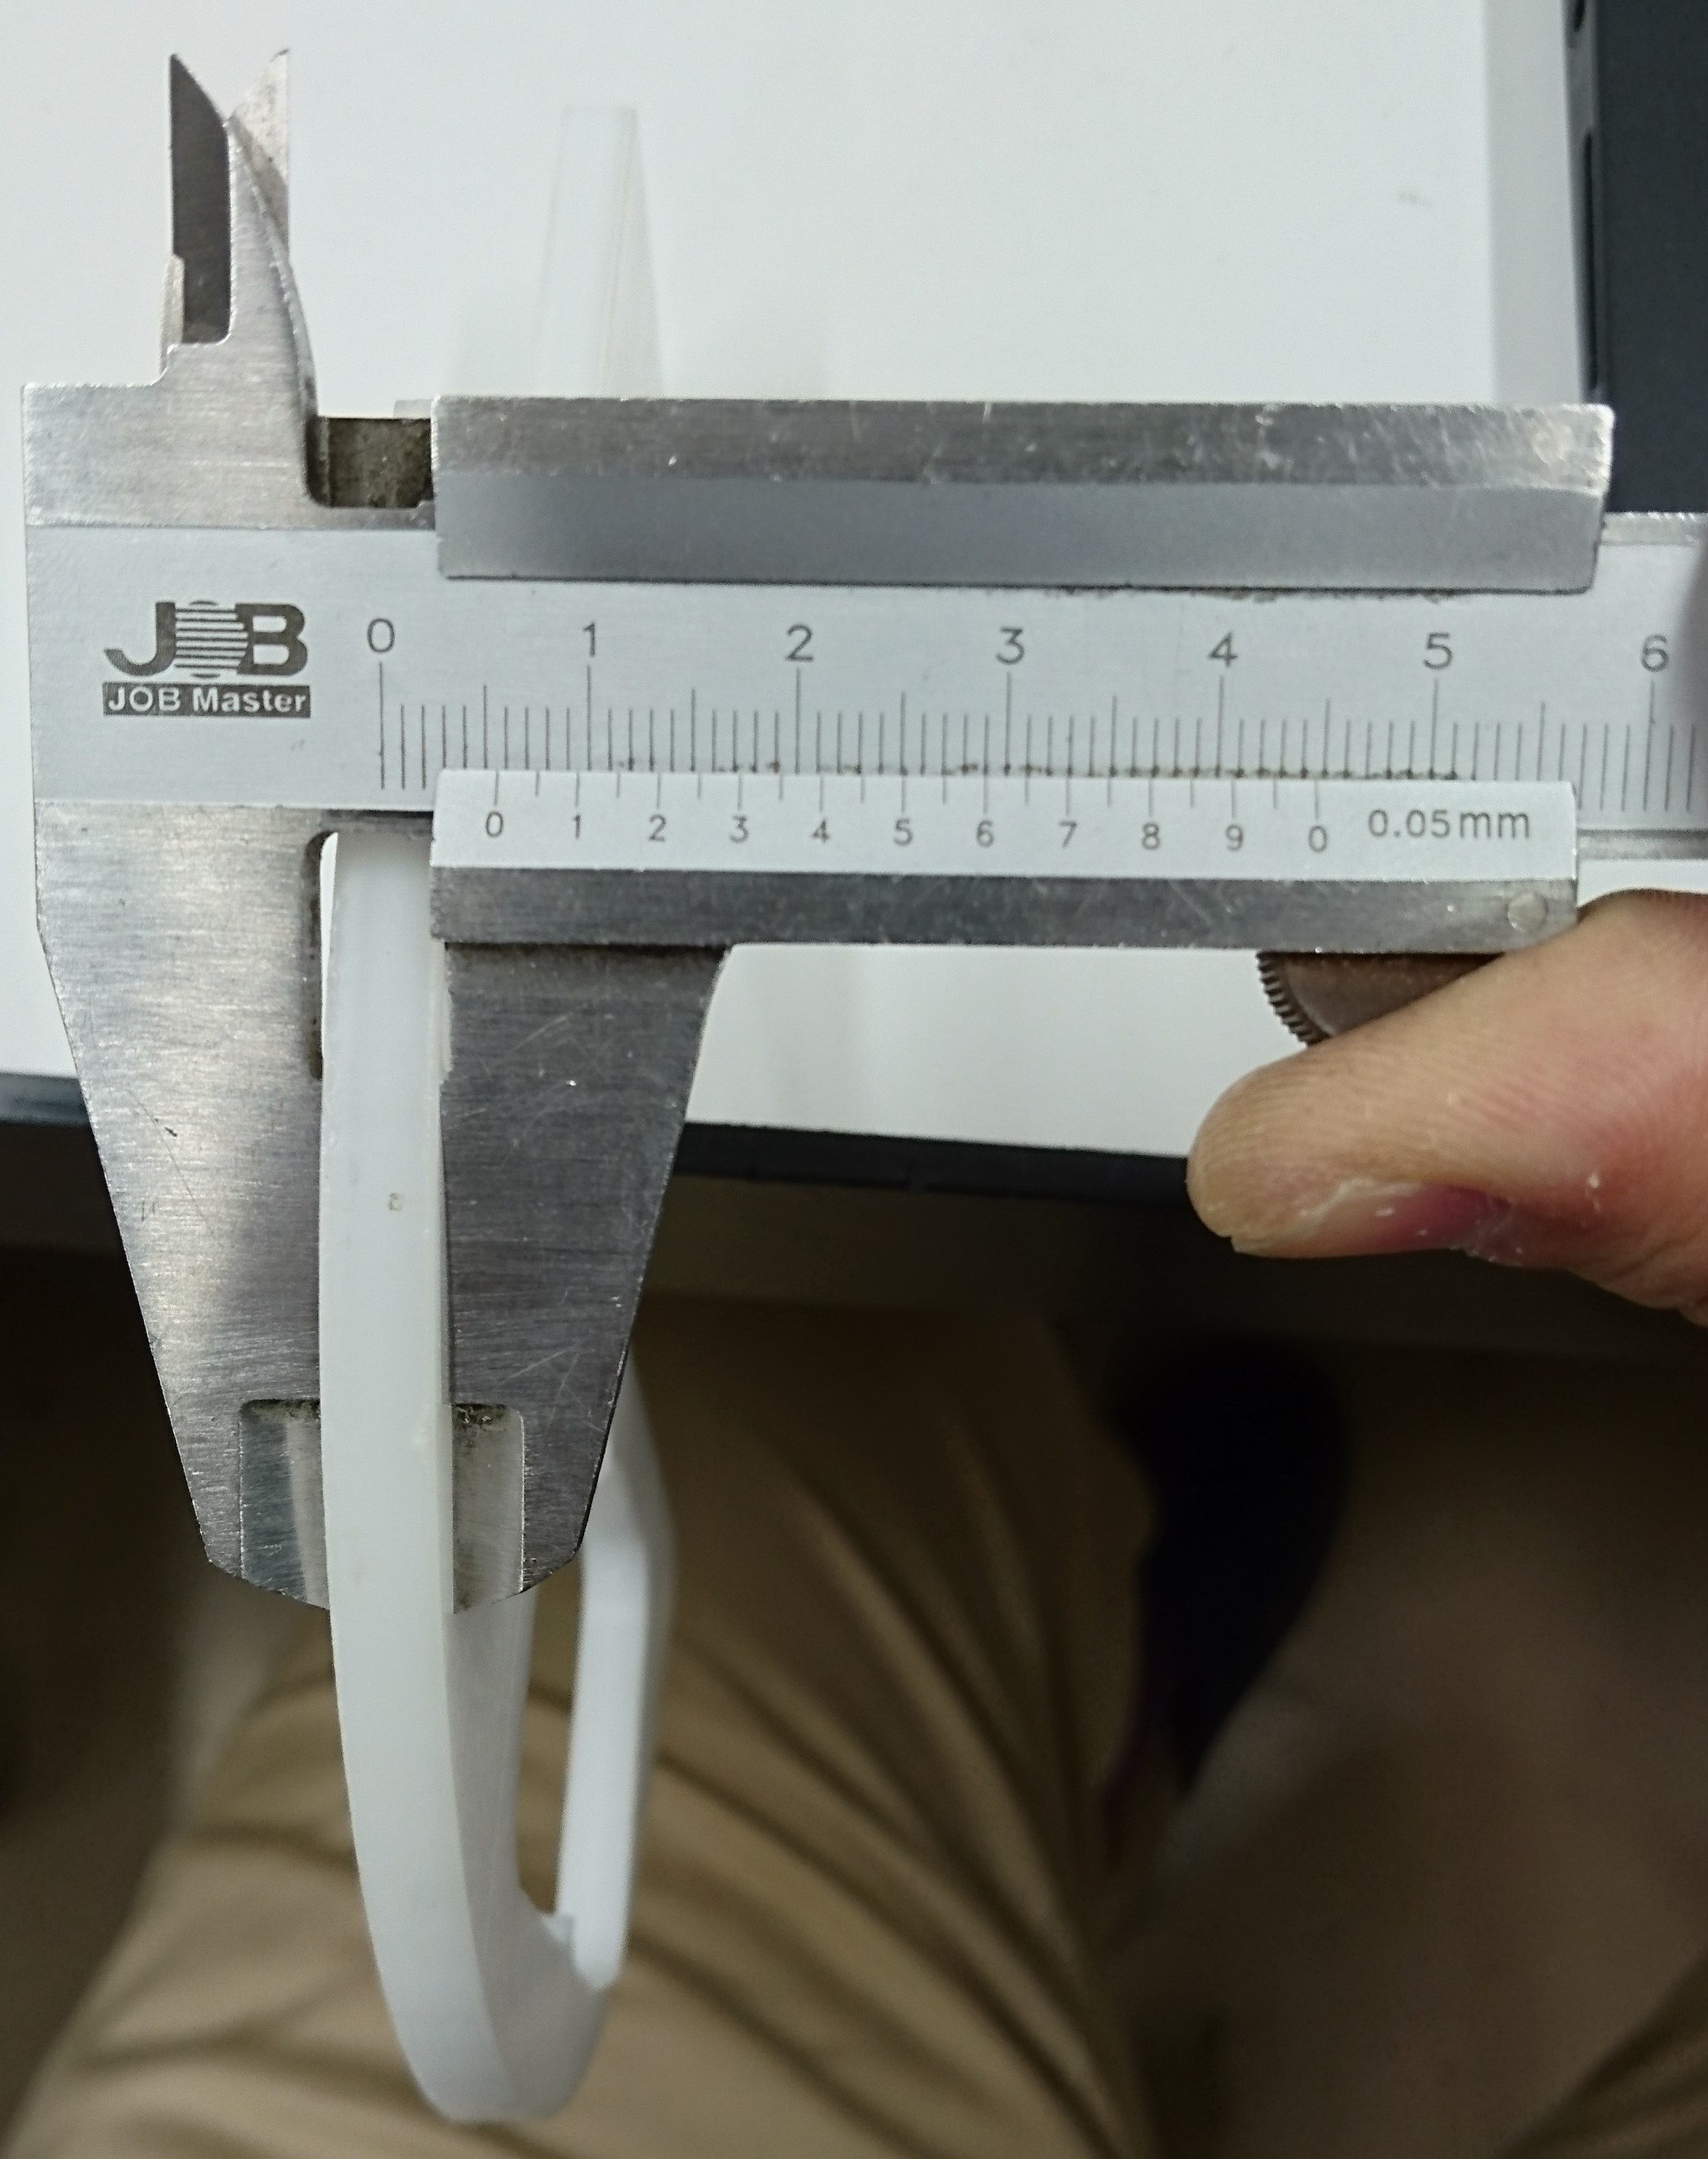
\includegraphics[width=\columnwidth]{nogisu_measure.jpg}
%%     \end{minipage}
%%     \caption{樹脂板の厚み計測    \label{nogisu_measure}}
%%   \end{center}
%% \end{figure*}

\begin{figure*}[tbh]
  \begin{center}
    \begin{minipage}{1.0\columnwidth}
      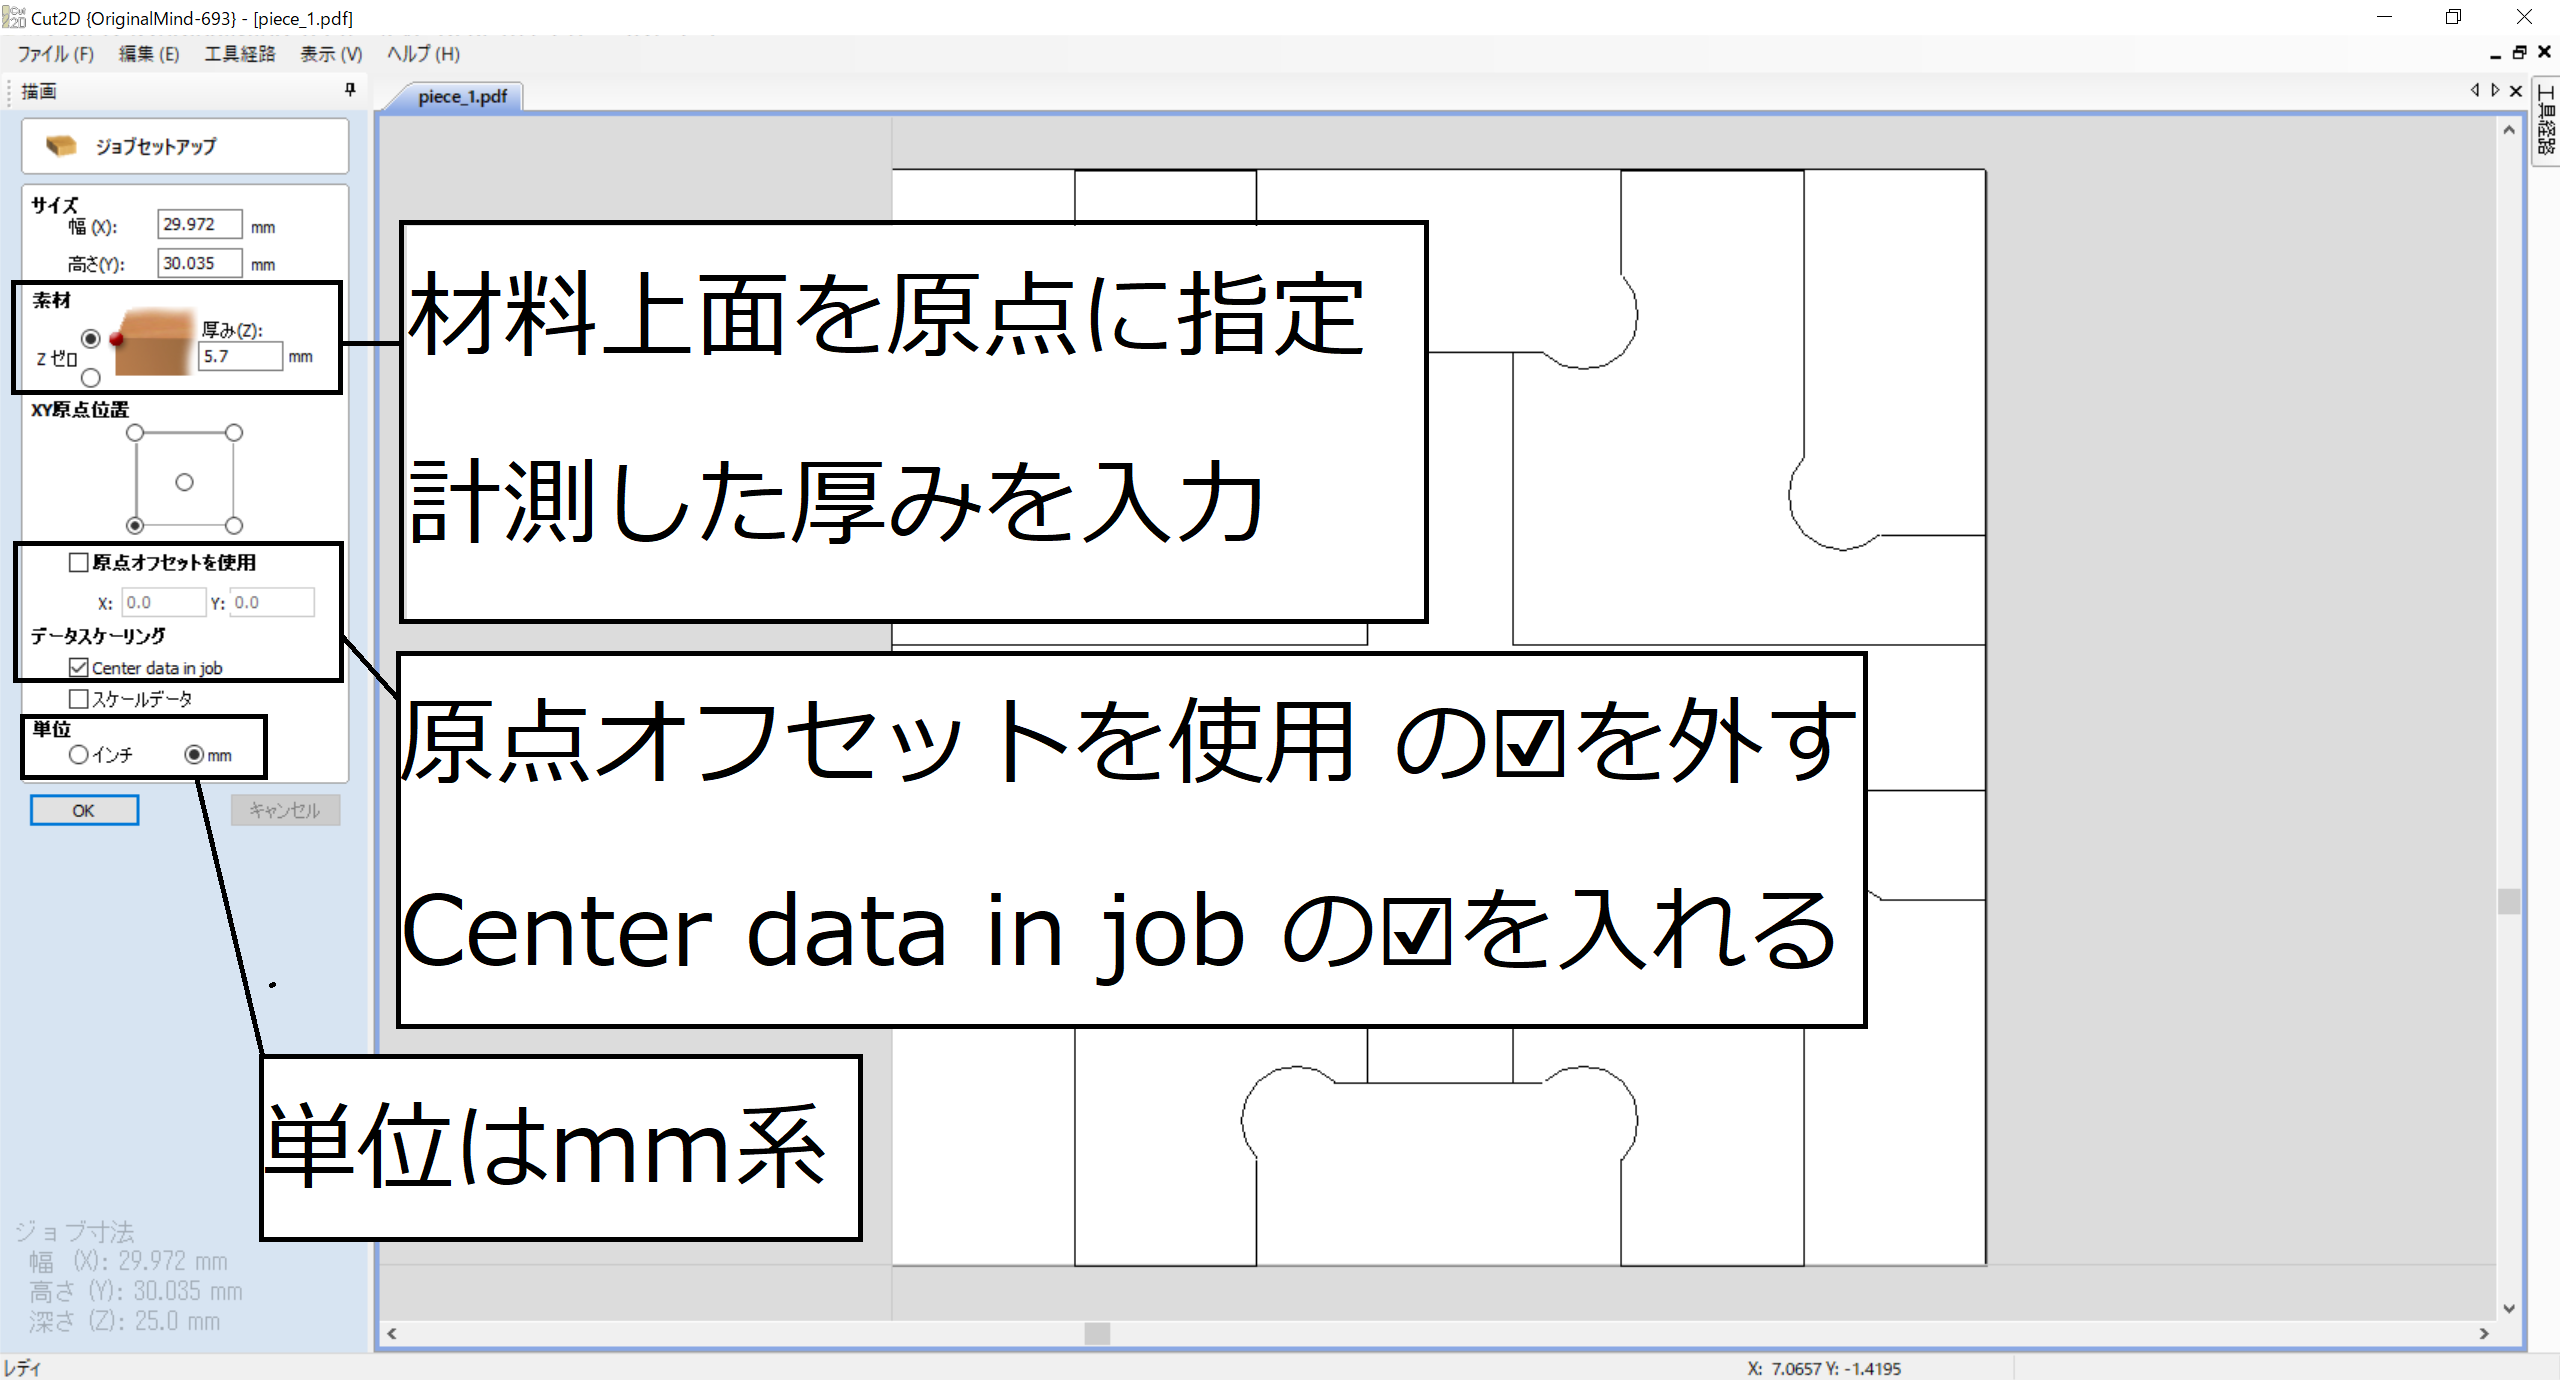
\includegraphics[width=\columnwidth]{first_setting.png}
    \end{minipage}
    \caption{初期設定    \label{first_setting}}
  \end{center}
\end{figure*}

%%画像*2 ノギスで厚みを測る写真 初期設定の画像 nogisu_measure.jpg first_setting.png

\clearpage
\subsection{ベクトルの編集}

厚みを入力したら、ベクトルの修正(追加、削除)を行います。Cut2Dのボタンは図\ref{button}のようになっています。ここでは、穴径の修正を取り上げます。外形の線に沿ってエンドミルが動くという性質から、エンドミルの直径と同じ径の穴をあけることは基本的にできません。穴径を空けたい径よりほんの少しだけ大きくすることで、この問題は解決できます。具体的な例を挙げると、Φ3のエンドミルを使って切削を行う場合、それと同じ径の穴は開けられないため、新しくΦ3.2の円形のベクトルを作って元の穴円のベクトルと中心が合うように配置することで、およそΦ3の穴をあけることができます。図\ref{circle_vector}のように、cut2dではデフォルトで円形の中心にカーソルをスナップしてくれるので、新しくベクトルを配置するのが容易です。また、部品の設計の時に、角の内側の切り抜きを忘れた場合などにも、ここで新しくベクトルを追加することで修正が可能です。その他、四角形やポリラインなど、様々な形のベクトルを追加することができるので、適宜試してみてください。また、ベクトル形式ファイルを出力する際に、前述の図表や隠線などの余計な線を消し忘れた場合も、ここで削除を行ってください。複数のベクトルを削除したい場合、ドラッグで範囲選択、shiftを押しながらクリックで複数選択、ctrl-aで全選択をできたりするので、適宜使用してください。\\

\begin{figure*}[tbh]
  \begin{center}
    \begin{minipage}{1.0\columnwidth}
      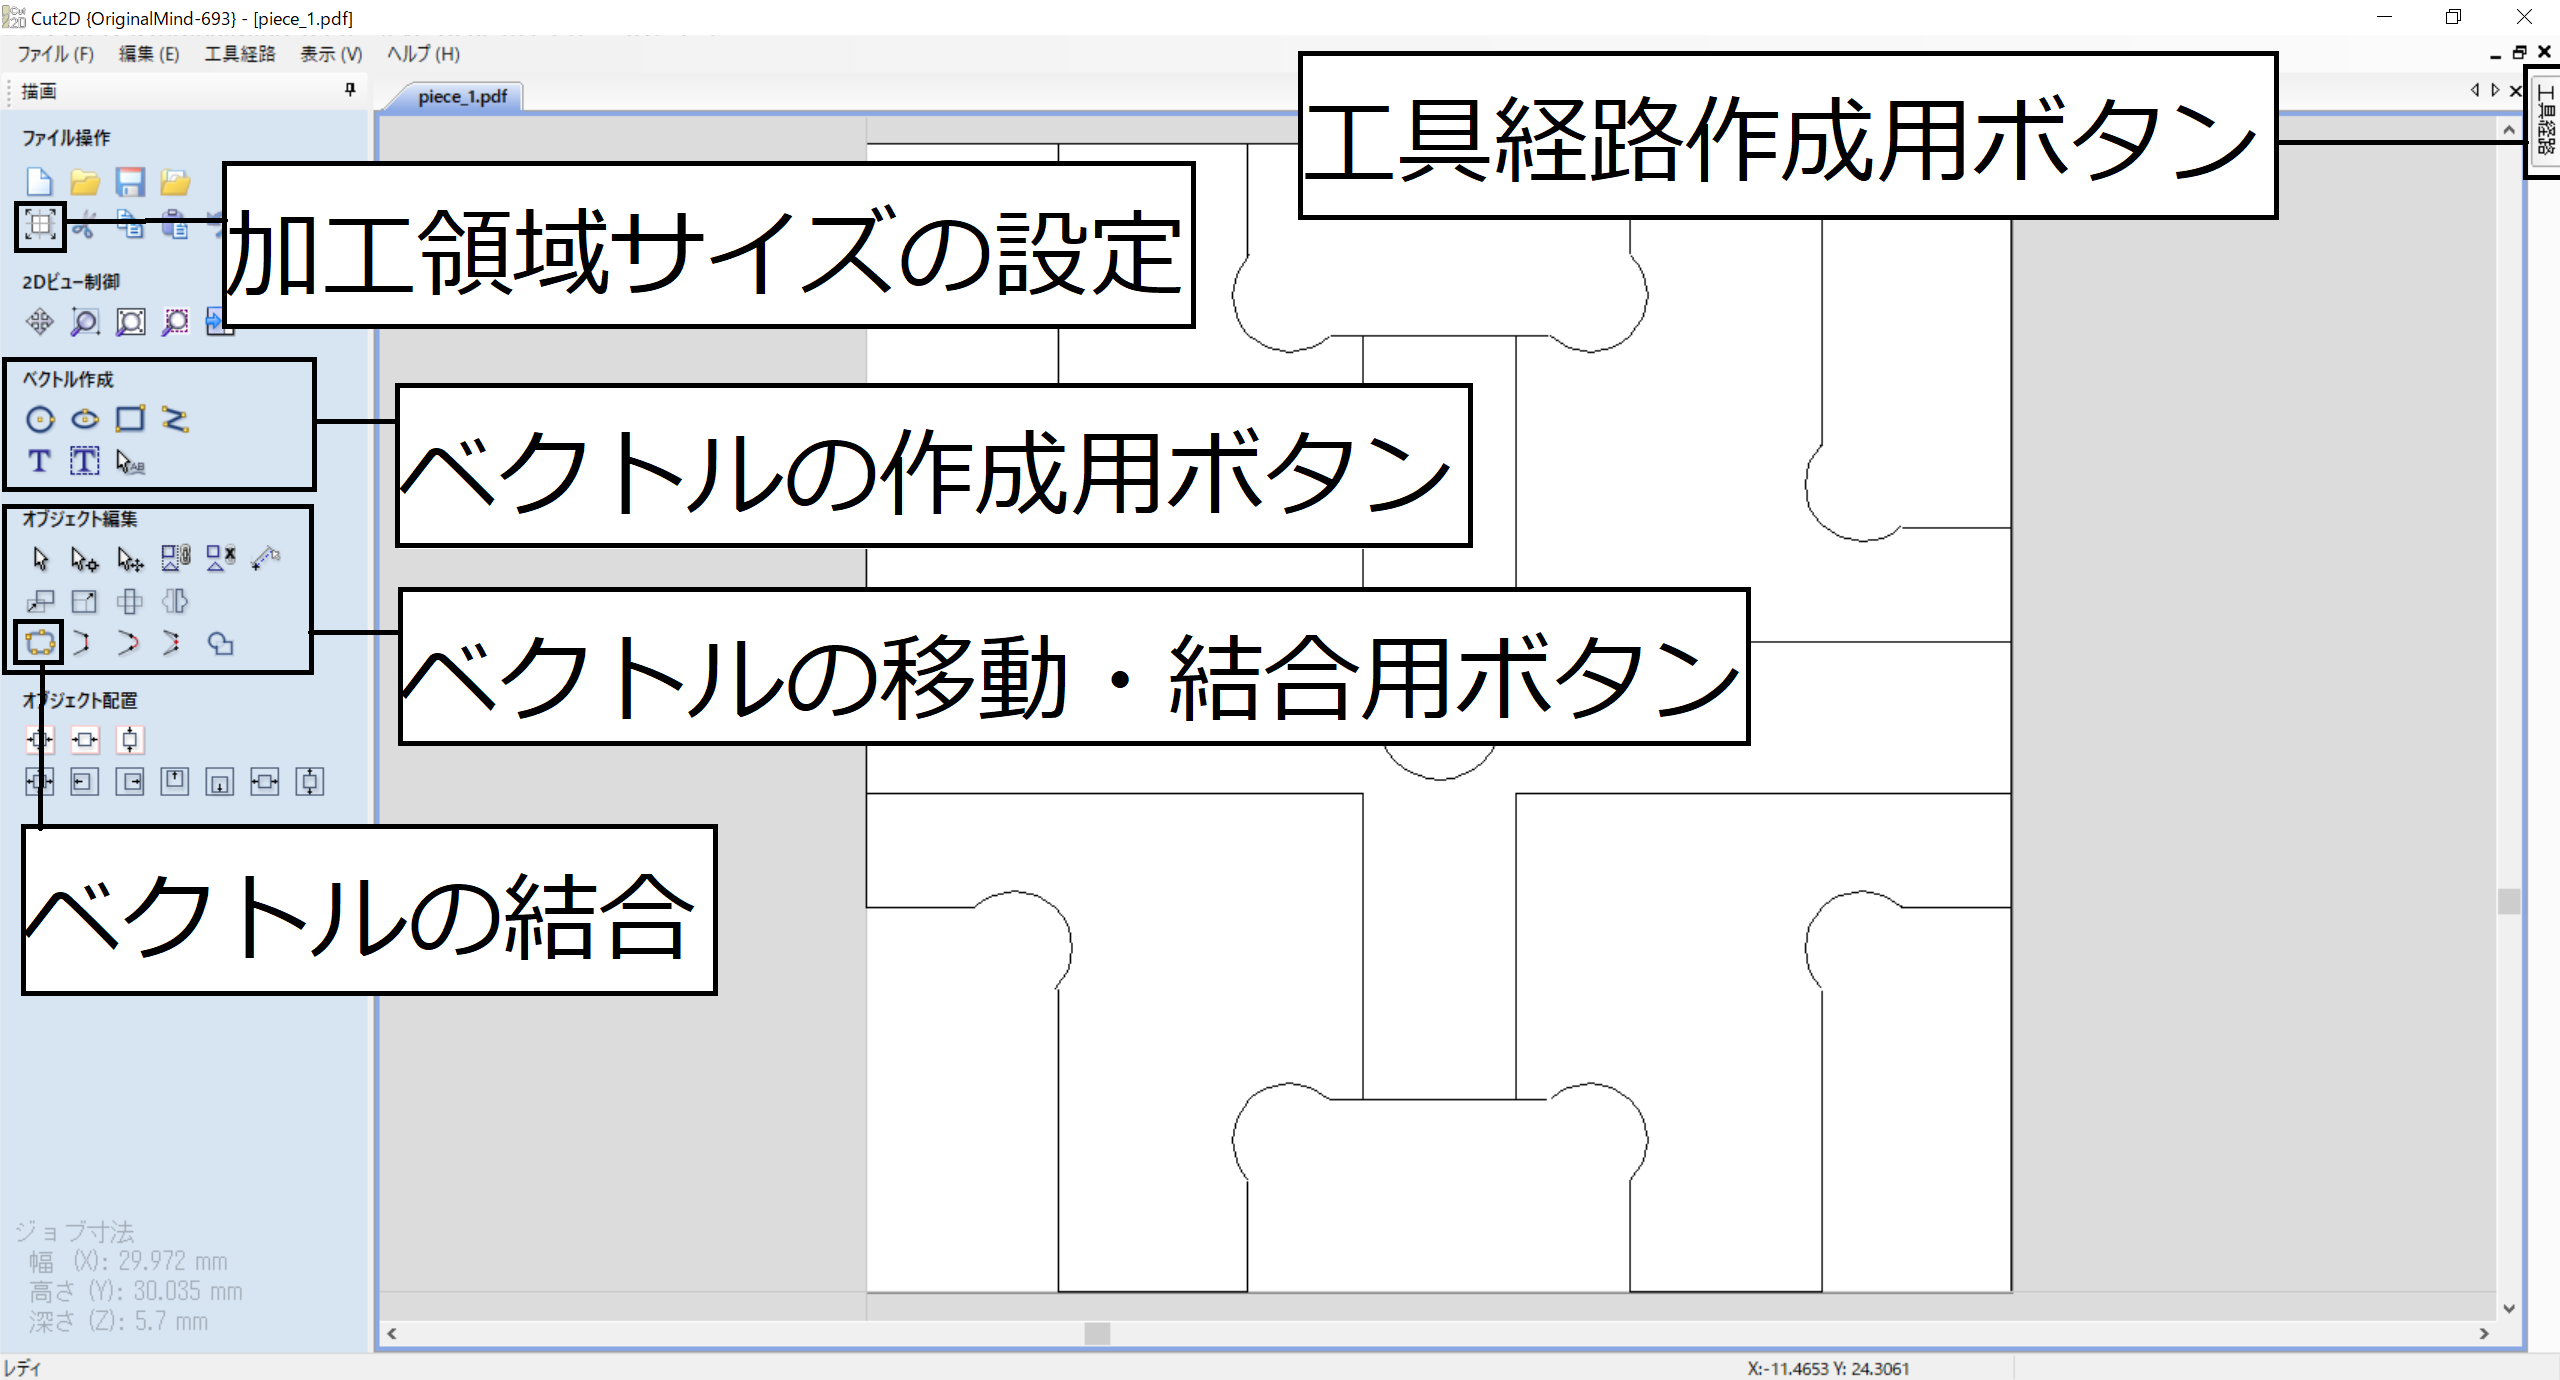
\includegraphics[width=\columnwidth]{button.png}
    \end{minipage}
    \caption{Cut2Dのボタン    \label{button}}
  \end{center}
\end{figure*}

\begin{figure*}[tbh]
  \begin{center}
    \begin{minipage}{1.0\columnwidth}
      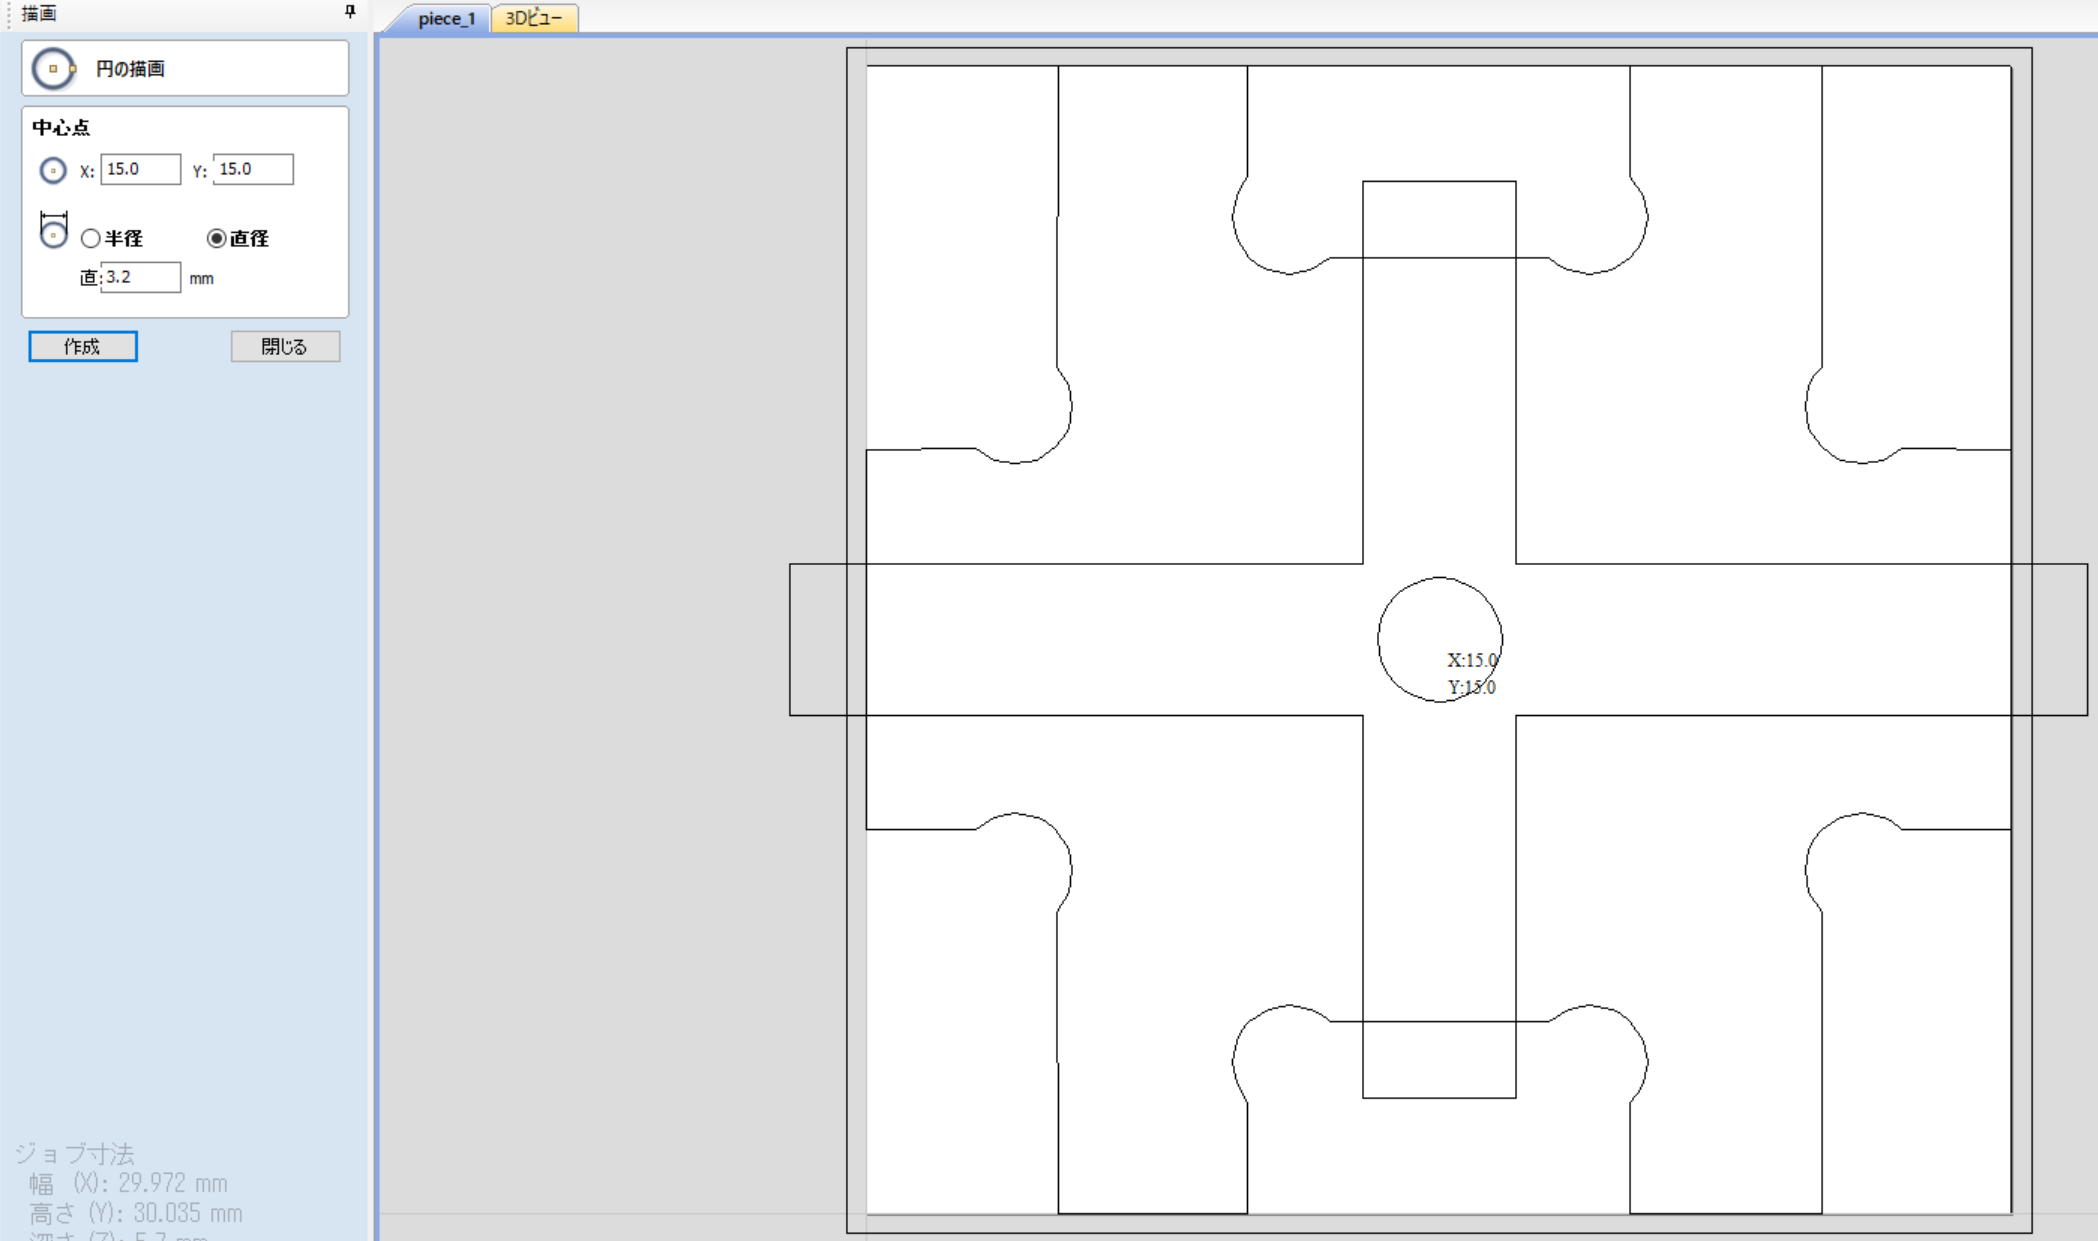
\includegraphics[width=\columnwidth]{circle_trim.png}
    \end{minipage}
    \caption{円形ベクトルの追加    \label{circle_vector}}
    \begin{minipage}{1.0\columnwidth}
      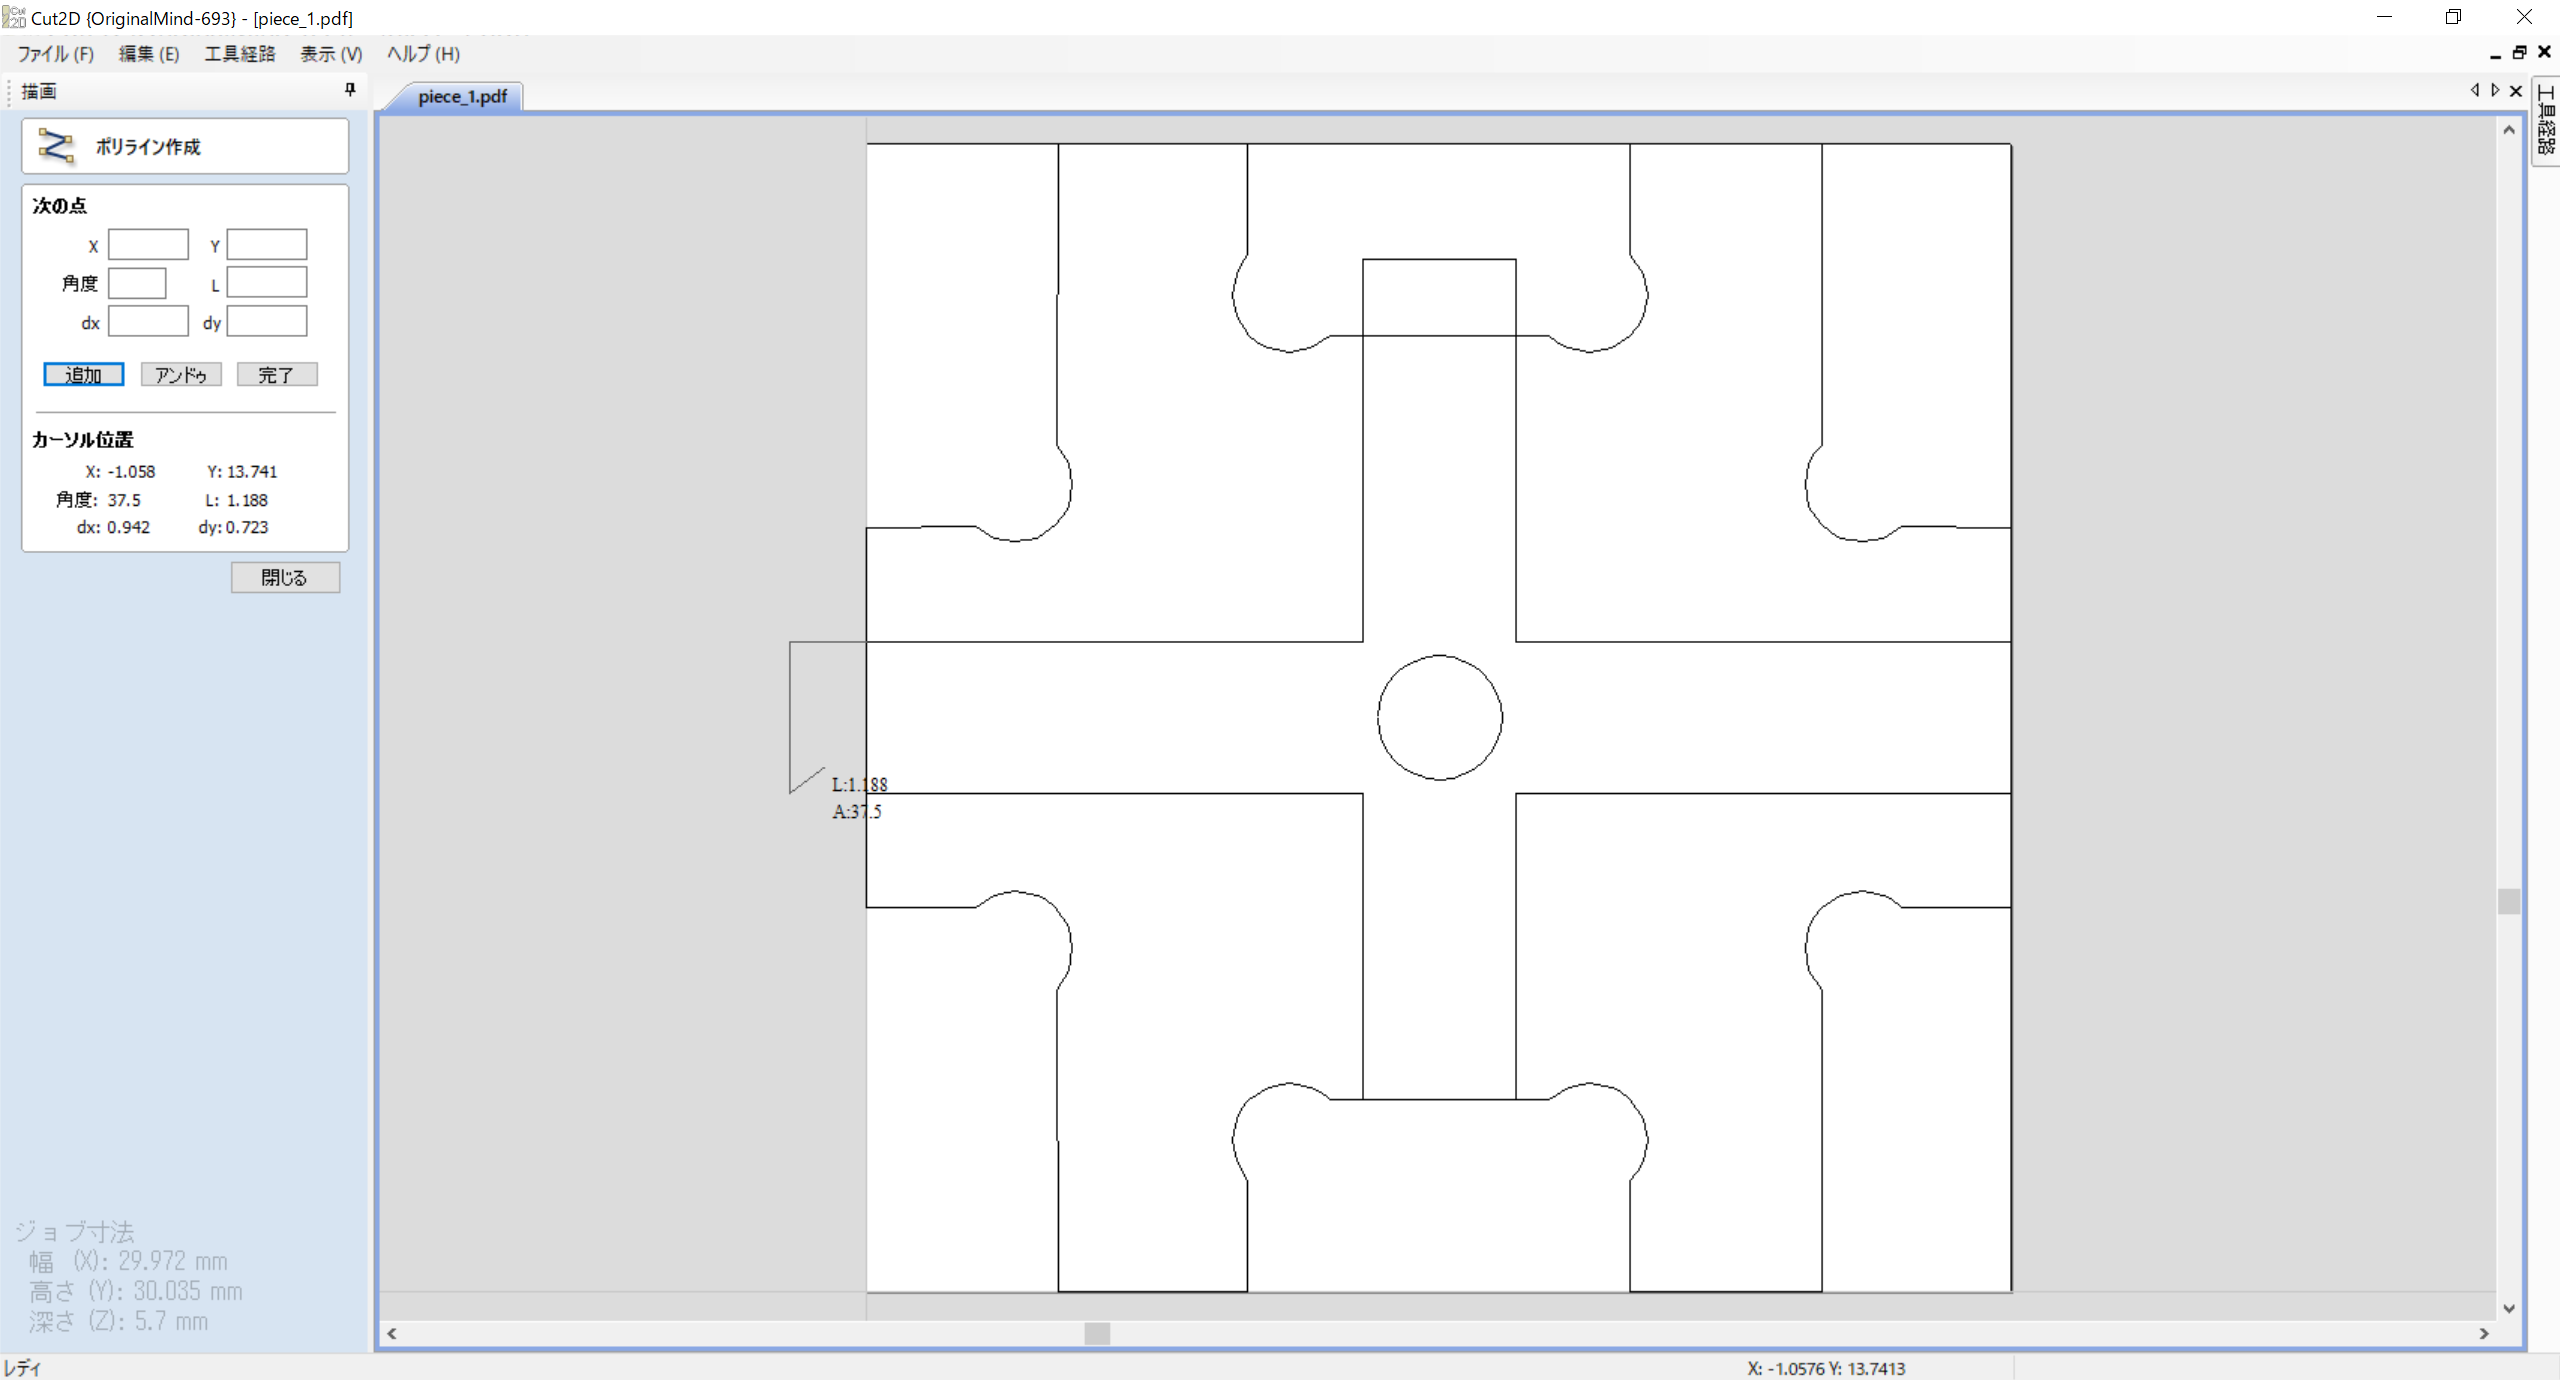
\includegraphics[width=\columnwidth]{polyline.png}
    \end{minipage}
    \caption{ポリラインベクトルの追加    \label{polyline_vector}}
  \end{center}
\end{figure*}

%%画像 *3 円形ベクトルの追加、ポリラインの追加 circle.png polyline.png final_vector.png final_vector_exp.png

\clearpage
ベクトルの修正を行ったら、最後にベクトルの結合を行います。図\ref{connect}の操作により、ベクトルを繋げて削りたい領域を作っていきます。ベクトルの結合 のボタンを押したら、繋げたいベクトルを全て選択します。許容誤差を入力する場所がありますが、0.1mm程度に設定します。どの程度ベクトルを繋げたいかに応じて、適宜値は変更してください。結合ボタンを押してつながっていることを確認したら終了です。先ほどのベクトルの修正で追加したベクトルも結合が可能なため、それと併せることで領域を好きなように作ることができます。今回の部品の加工ファイルでは、加工に必要なベクトルを追加・結合して、最終的には以下の図\ref{final_vector}のようになります。\\

\begin{figure*}[tbh]
  \begin{center}
    \begin{minipage}{0.9\columnwidth}
      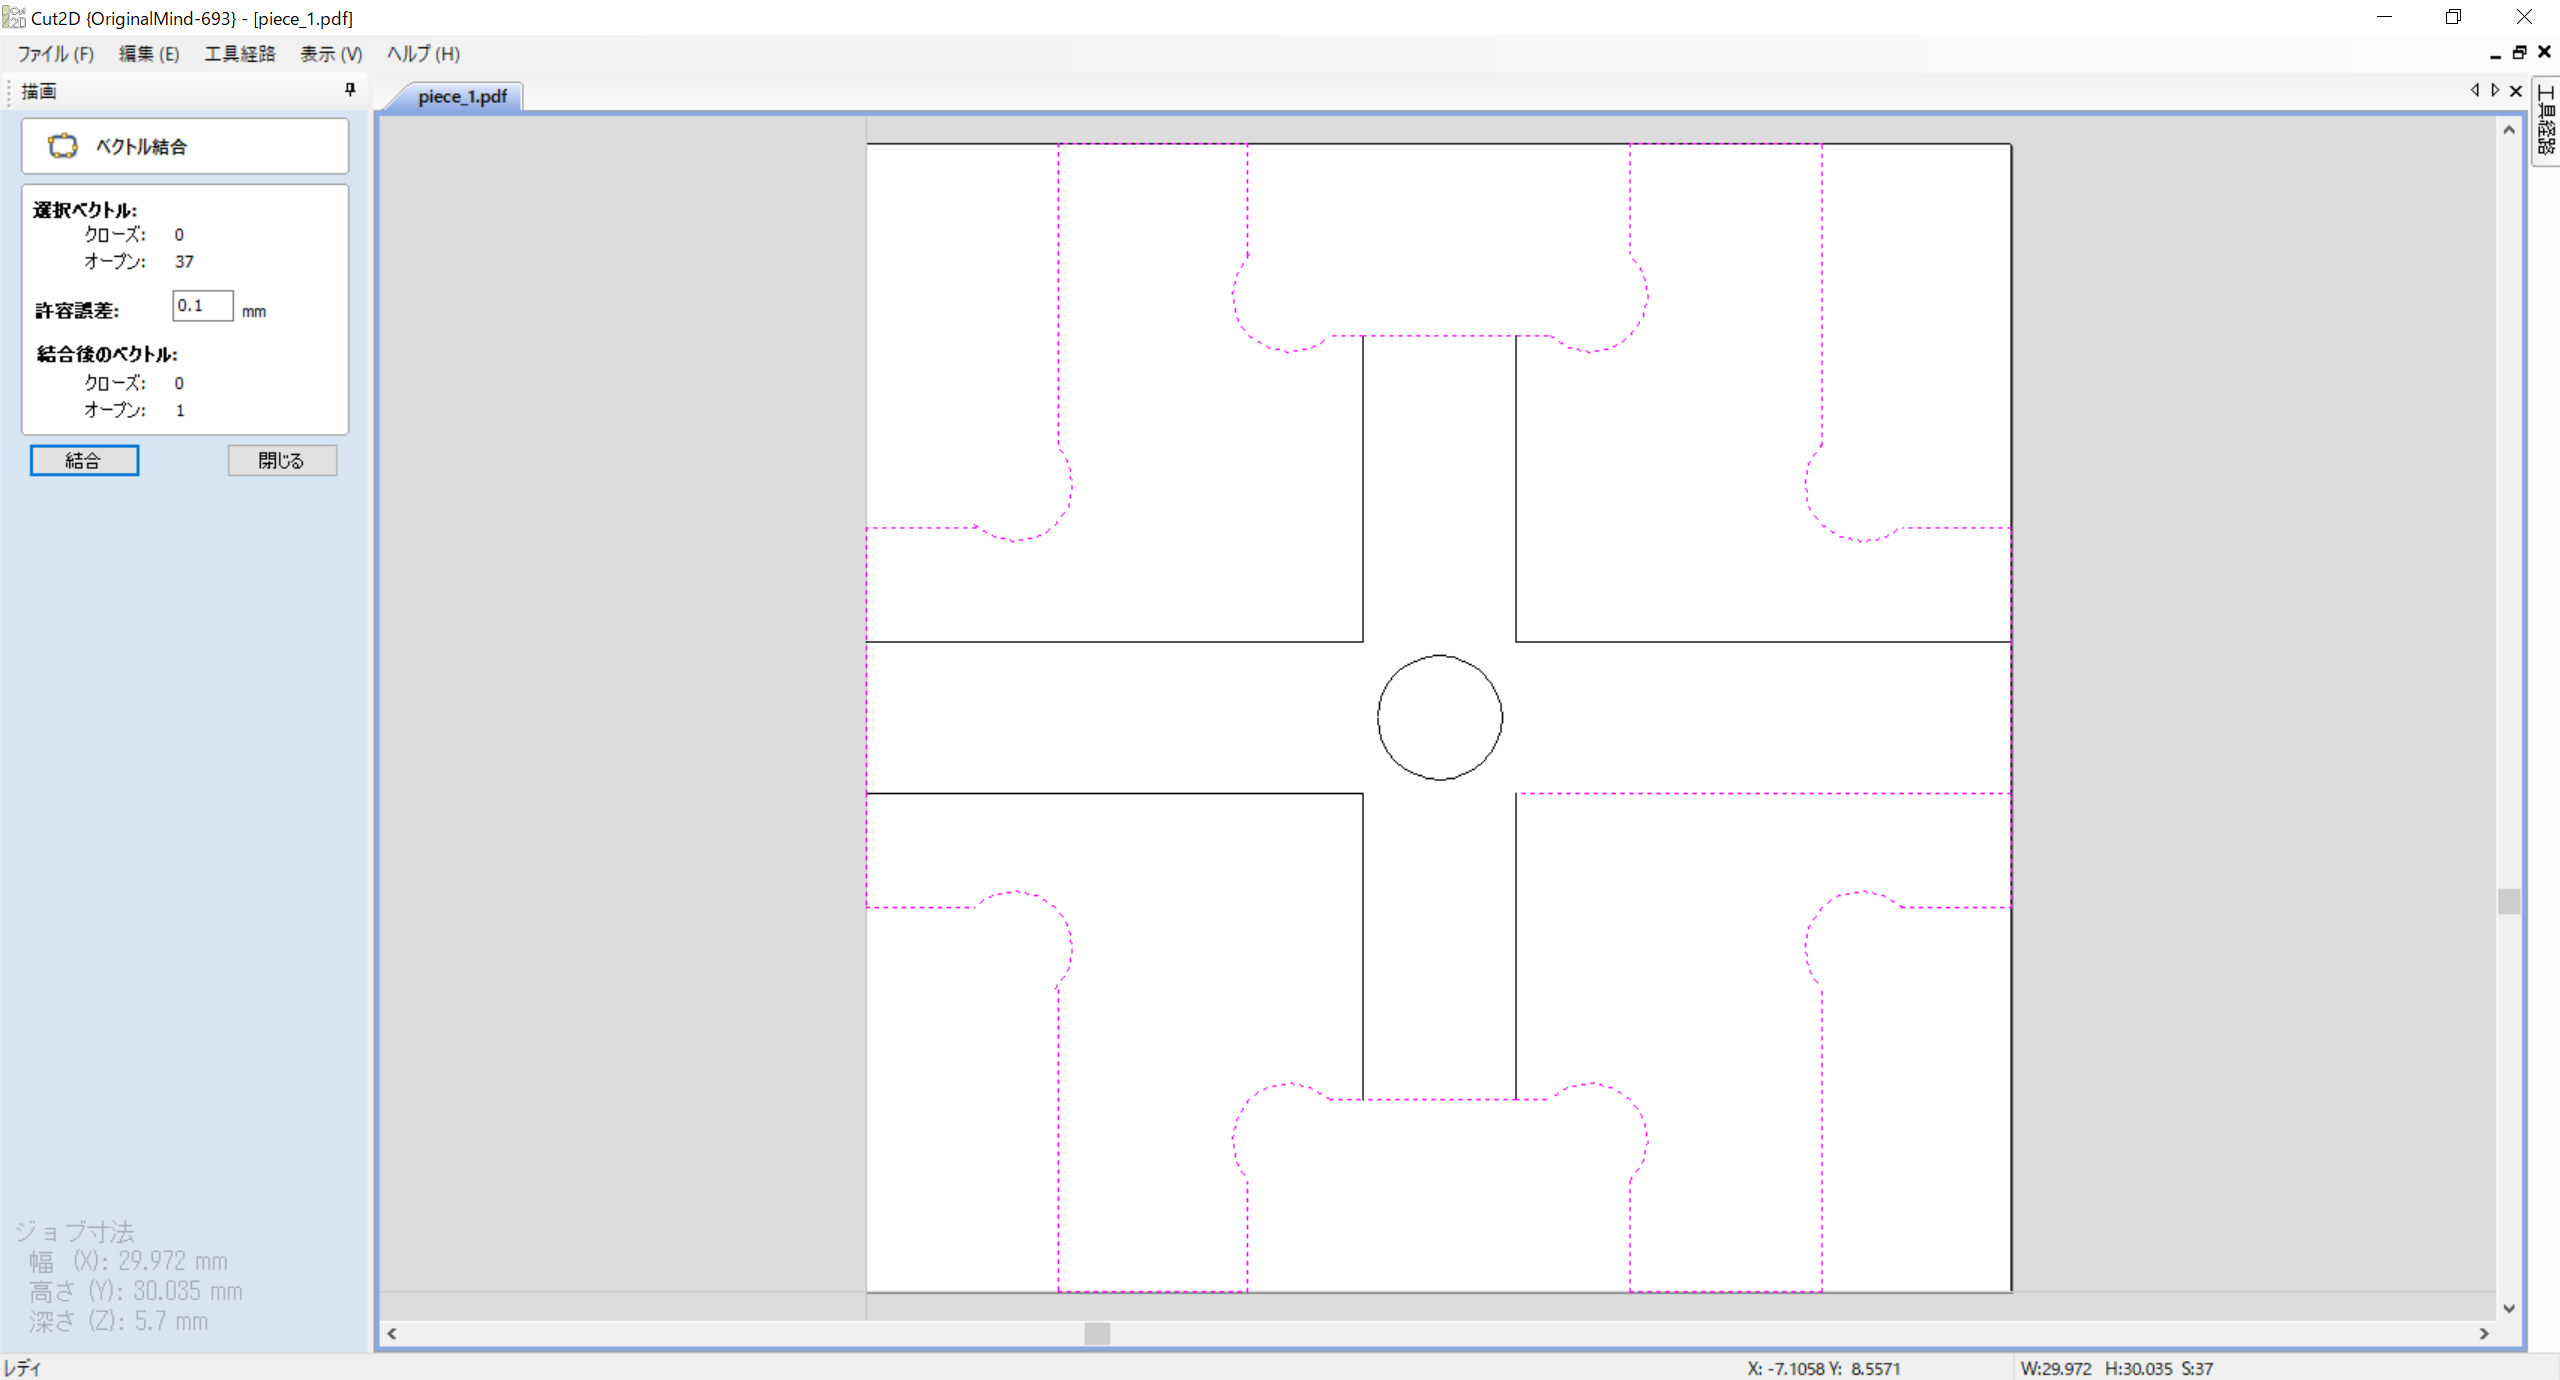
\includegraphics[width=\columnwidth]{vector_connect.png}
    \end{minipage}
    \caption{ベクトルの結合    \label{connect}}
    %% \begin{minipage}{0.6\columnwidth}
    %%   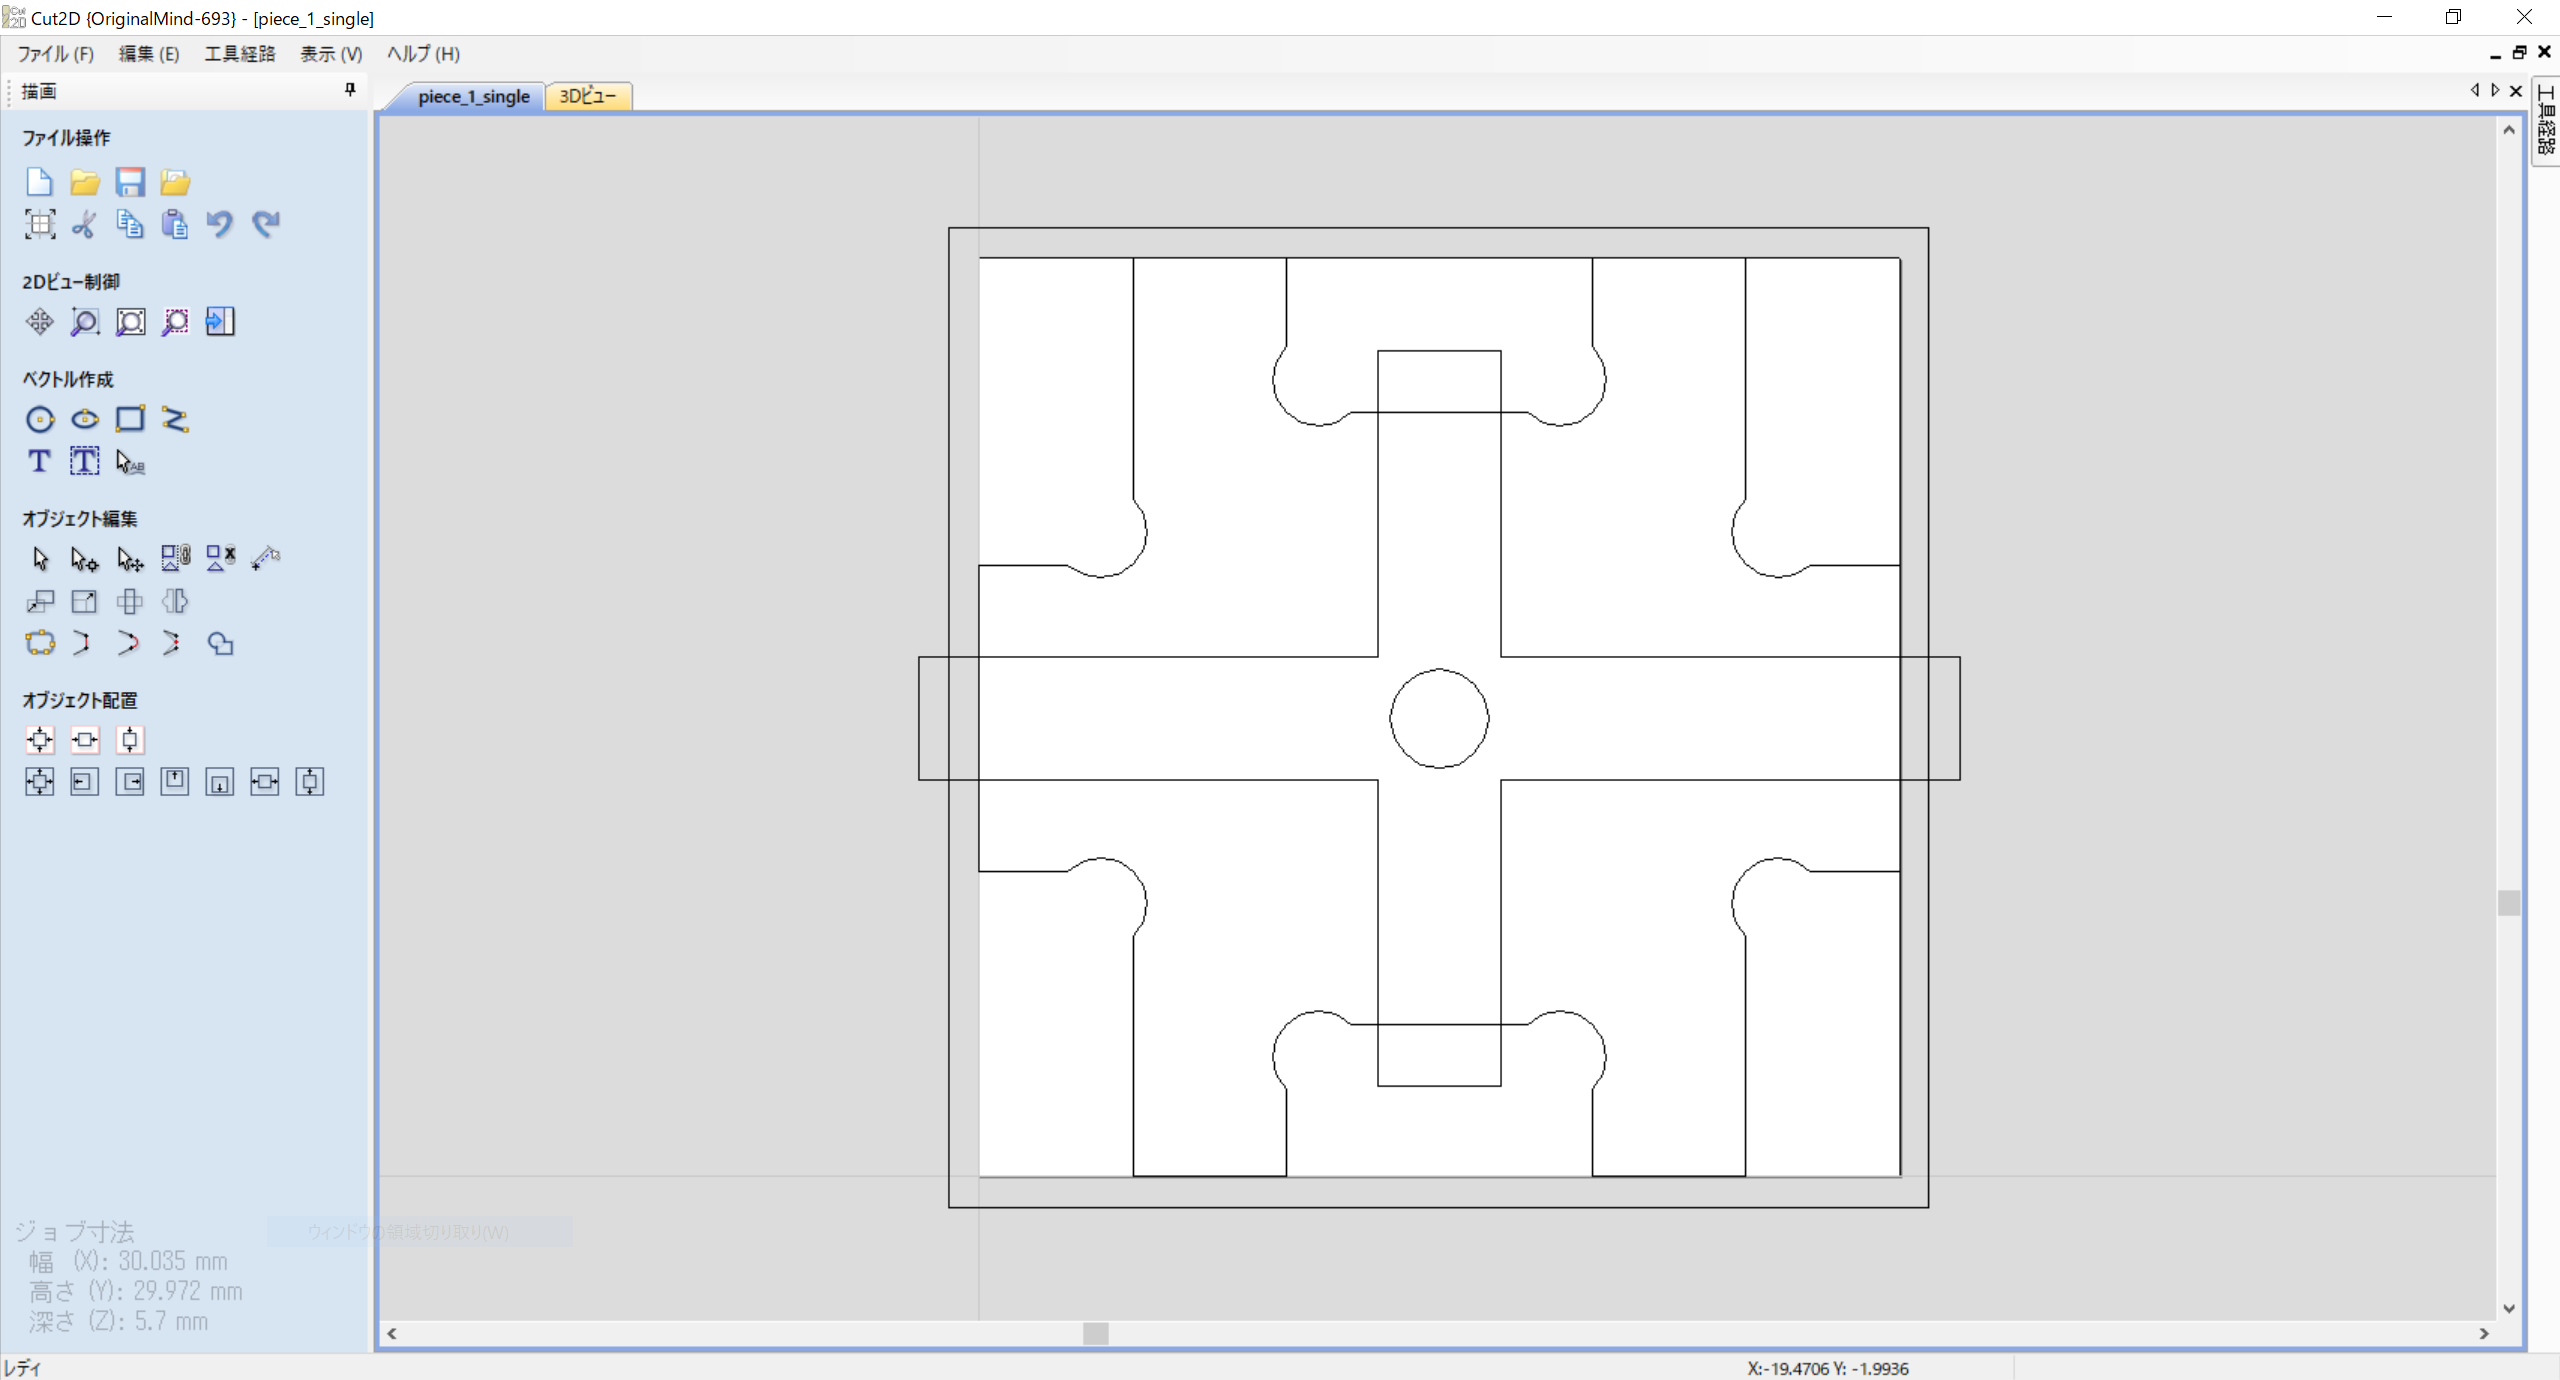
\includegraphics[width=\columnwidth]{final_vector.png}
    %% \end{minipage}
    \begin{minipage}{0.9\columnwidth}
      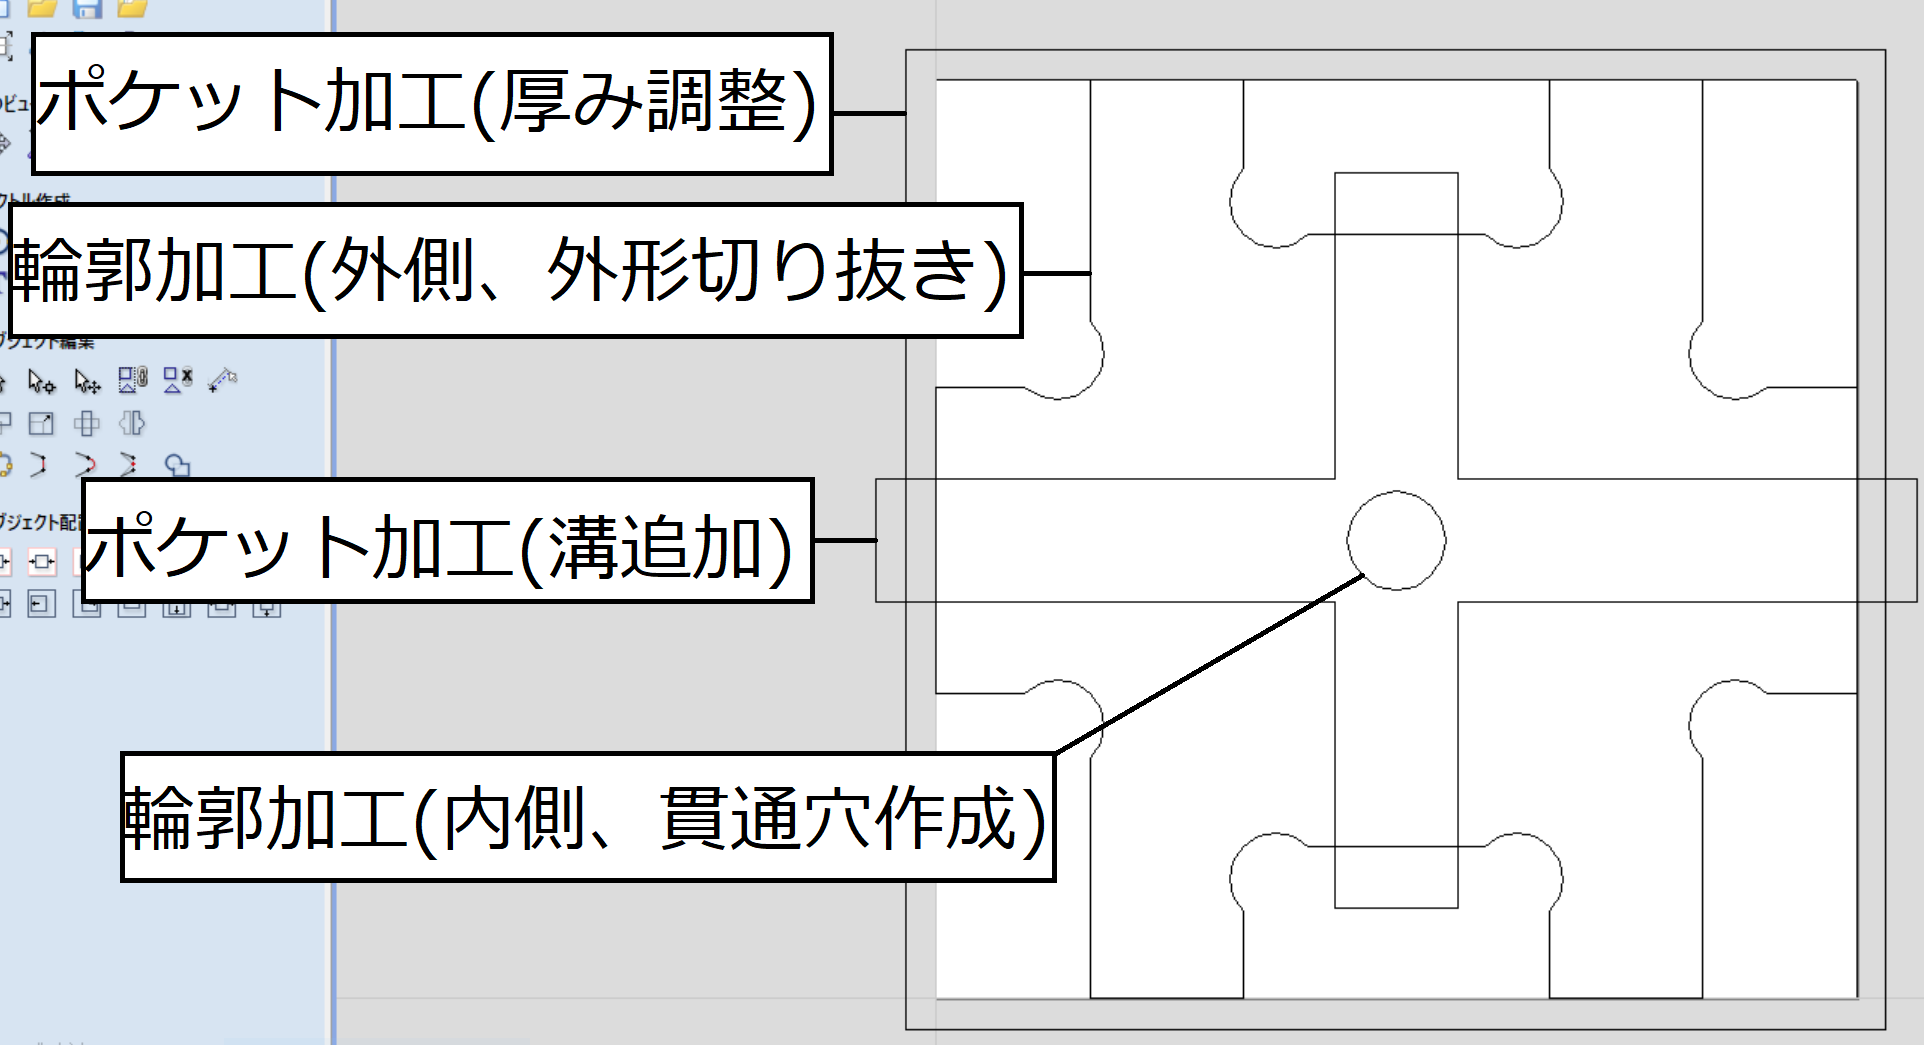
\includegraphics[width=\columnwidth]{final_vector_exp_trim.png}
    \end{minipage}
    \caption{最終的なベクトル    \label{final_vector}}
  \end{center}
\end{figure*}

%%画像*4 ボタンの説明の画像 ベクトルの結合の画像 最終的なベクトル  button.png vector_connect.png final_vector.png final_vector_exp.png

\clearpage
\subsection{経路作成}
ベクトルの編集が終わったら、経路の作成を行います。基本的な流れとしては、\\
  1.ベクトルの選択\\
  2.経路の種類の選択\\
  3.経路の計算\\
  4.経路の整理\\
  5.経路のプレビュー\\
  という順番で行います。\\

工具経路タブのボタンは図\ref{tool_button}のようになっています。まず経路の種類の選択を行います。経路には輪郭加工経路とポケット加工経路の2つの種類があります。\\
\begin{figure*}[tbh]
  \begin{center}
    \begin{minipage}{1.0\columnwidth}
      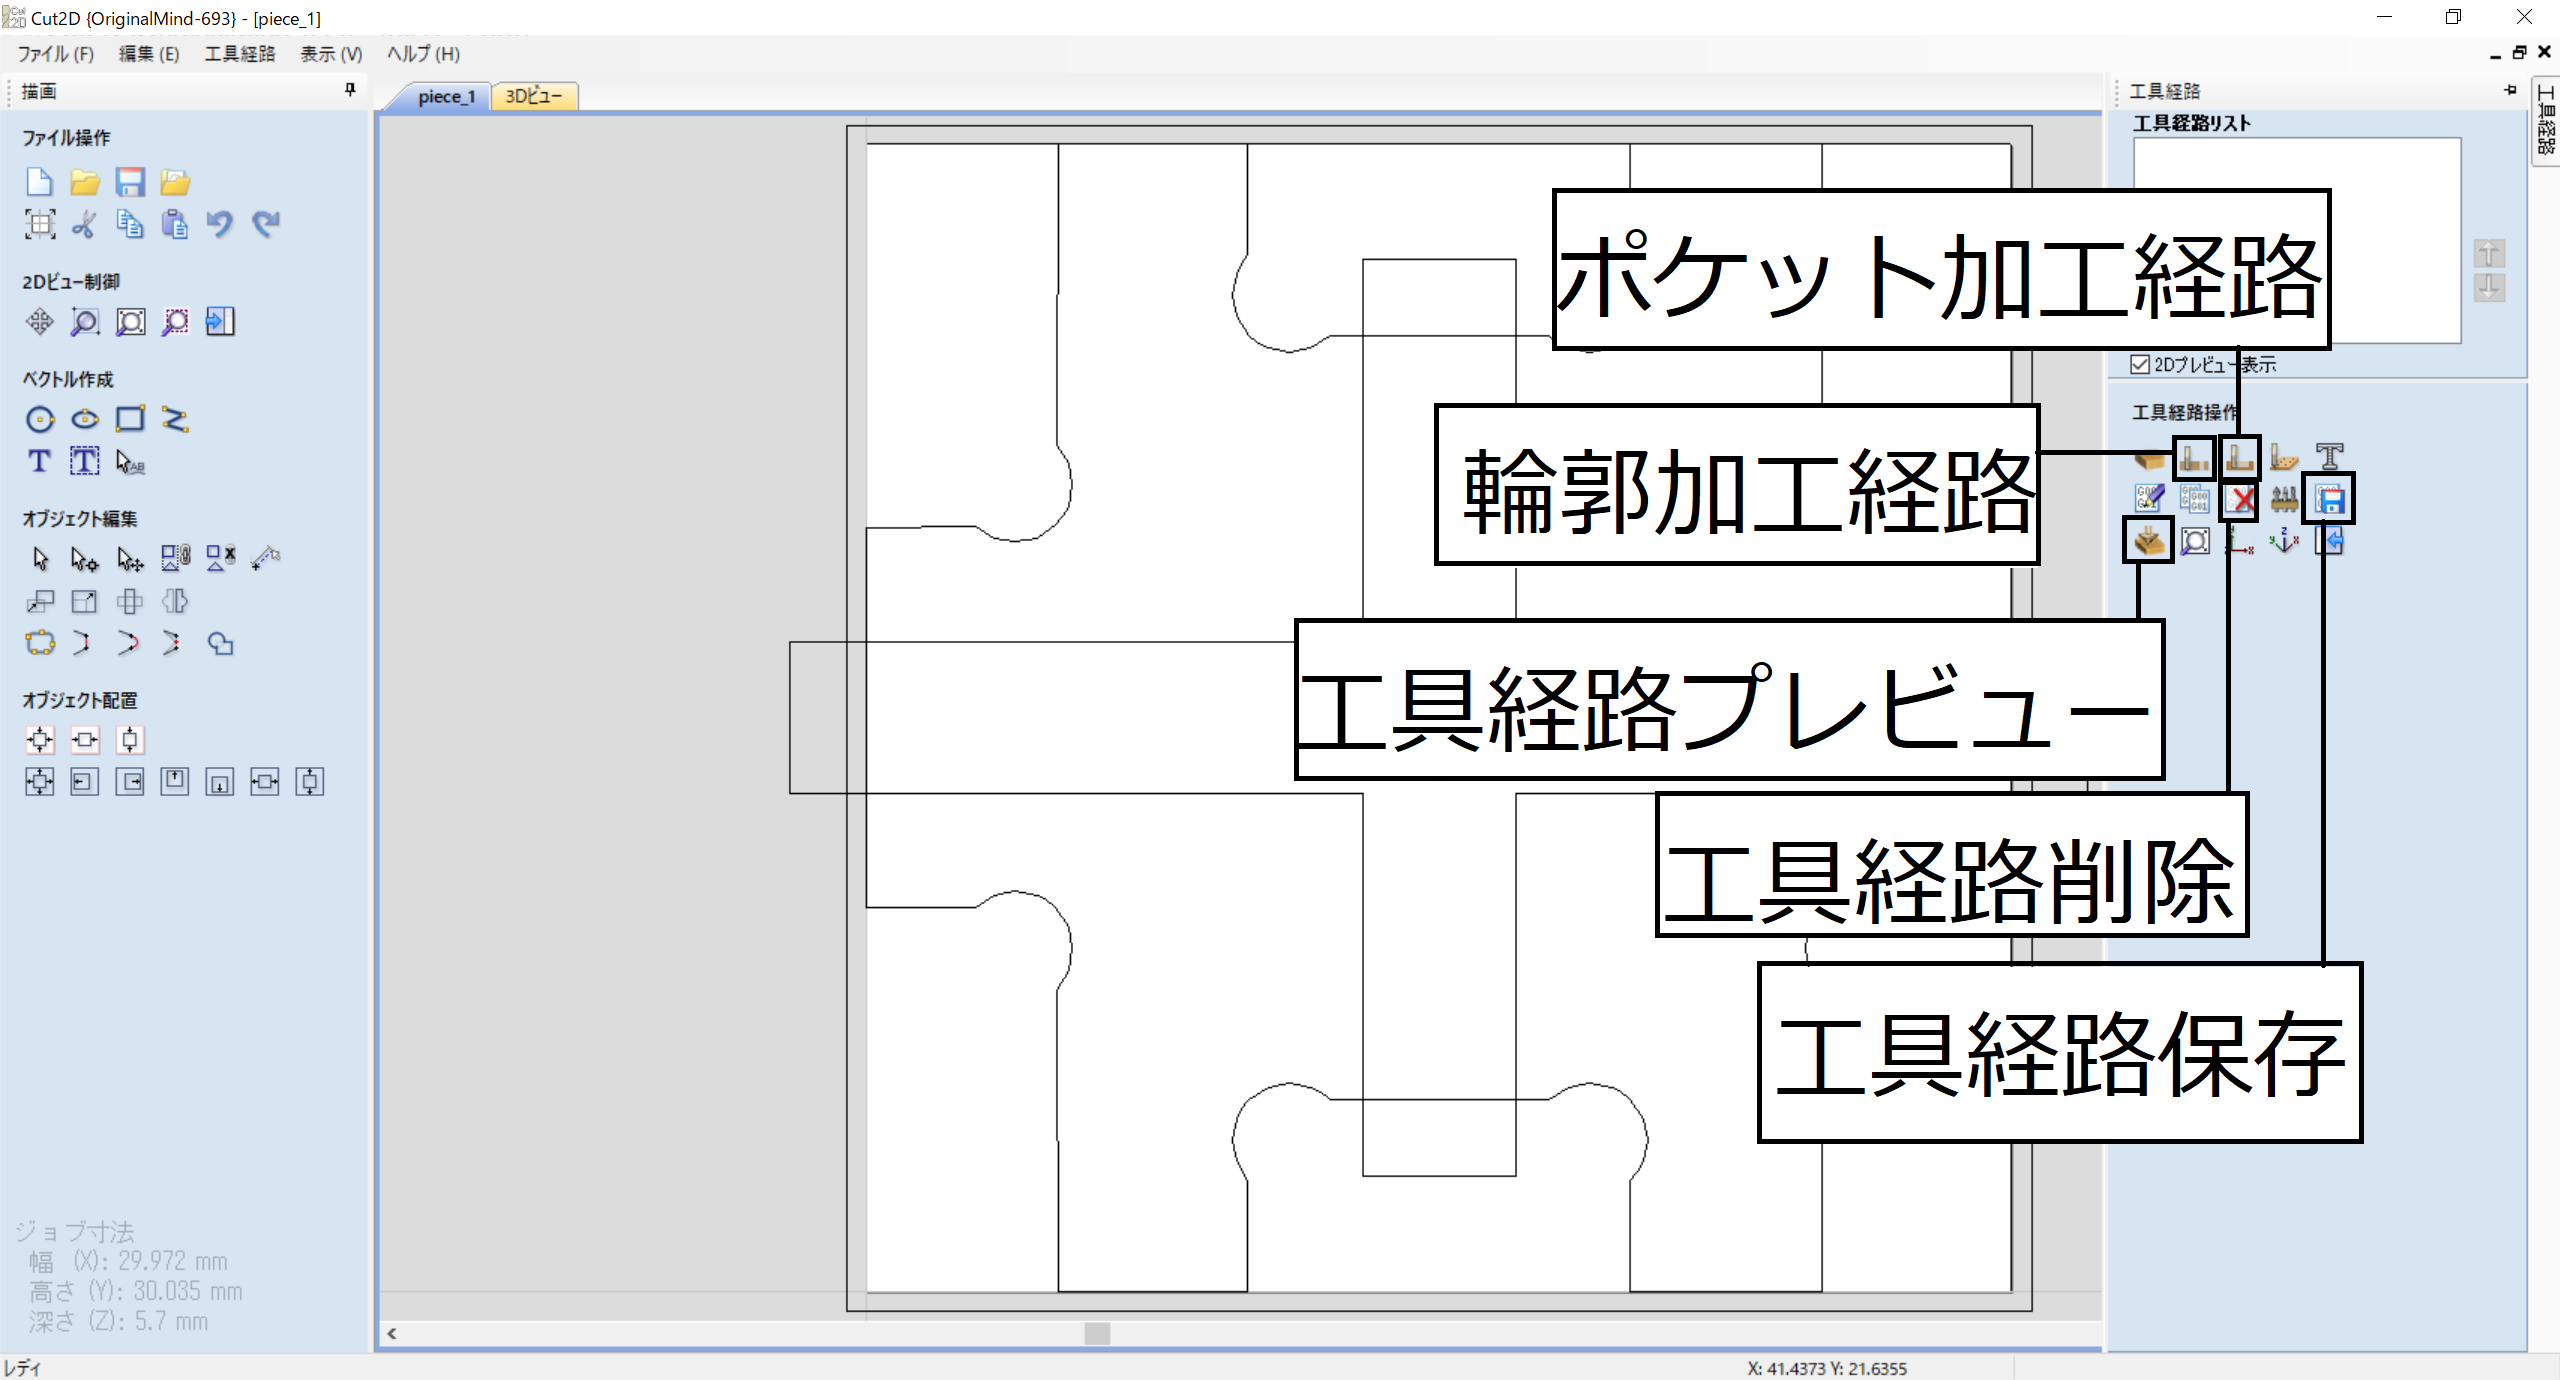
\includegraphics[width=\columnwidth]{tool_button.png}
    \end{minipage}
    \caption{工具経路ボタン    \label{tool_button}}
  \end{center}
\end{figure*}

\clearpage
図\ref{outer_milling}の輪郭加工経路は選択したベクトルに沿ってエンドミルが動く経路です。ベクトルに沿って加工を行うため、内周・外周の切削を行う場合は、ベクトルは閉じたベクトルである必要があります。経路を作る際にはベクトルを選択し、内側の加工か、外側の加工かを選択してください。また、ベクトルの中心を通る経路も作ることが可能であり、こちらは閉じたベクトルである必要はありません。これは模様や名前の刻印等に使うことができます。\\

\begin{figure*}[tbh]
  \begin{center}
    \begin{minipage}{1.0\columnwidth}
      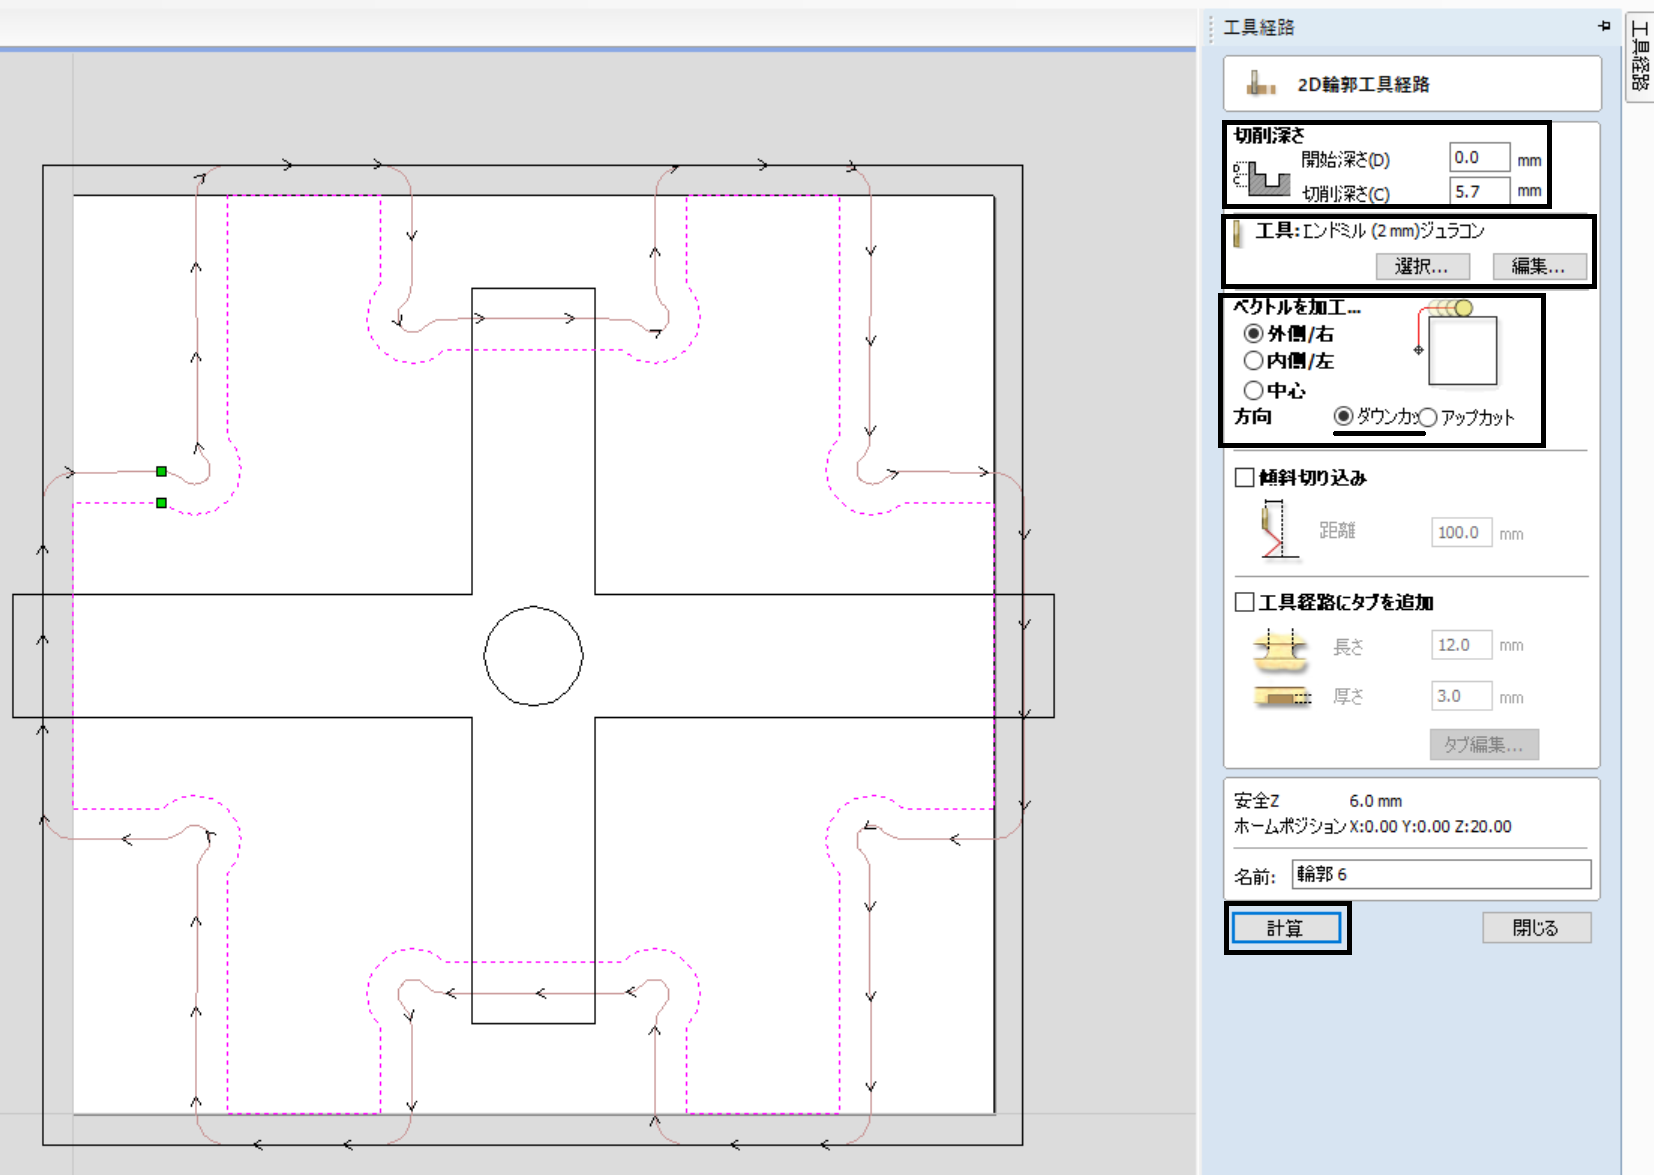
\includegraphics[width=\columnwidth]{outer_milling_trim.png}
    \end{minipage}
    \caption{輪郭加工経路    \label{outer_milling}}
  \end{center}
\end{figure*}

%%画像*2 工具経路ボタンの説明 輪郭加工経路 tool_button.png outer_milling_trim.png

\clearpage
一方、図\ref{pocket_milling}のポケット加工経路は選択したベクトルの内部をすべて削る経路です。これは、広い範囲を削って部品の厚みを変えたり、くぼみを作って他の部品をはめ込むような部品を作ることができます。この加工を行う際には、閉じた領域を指定する必要があるため、ベクトルは閉じている必要があります。また、ポケット加工経路にもオフセットとラスタの2種類が存在します。オフセットは領域内を中心から外側に向かってぐるぐると回るような経路で切削していくものです。こちらは、円形の領域や、x,y軸に対して斜めになった長方形の領域を削る時に有用です。さらに、エンドミル径とほぼ同じ径の小さい穴を深く掘る際にもポケット加工は有用です。これはエンドミルの形状が原因で、切り屑が穴の外に逃げにくくなっているため、ポケット加工で加工を行うことで、1層切削する度にエンドミルが穴から抜けて、切り屑が穴から外に出て溜まりにくくなるため、深く掘り進むのに向いています。一方、ラスターは左右に往復しつつ手前から奥に向かってに削っていくものになります。CNCのx,y軸方向に伸びる長方形の領域を削る場合には、方向を変更する回数が少ないこの方式が向いています。\\

\begin{figure*}[tbh]
  \begin{center}
    \begin{minipage}{1.0\columnwidth}
      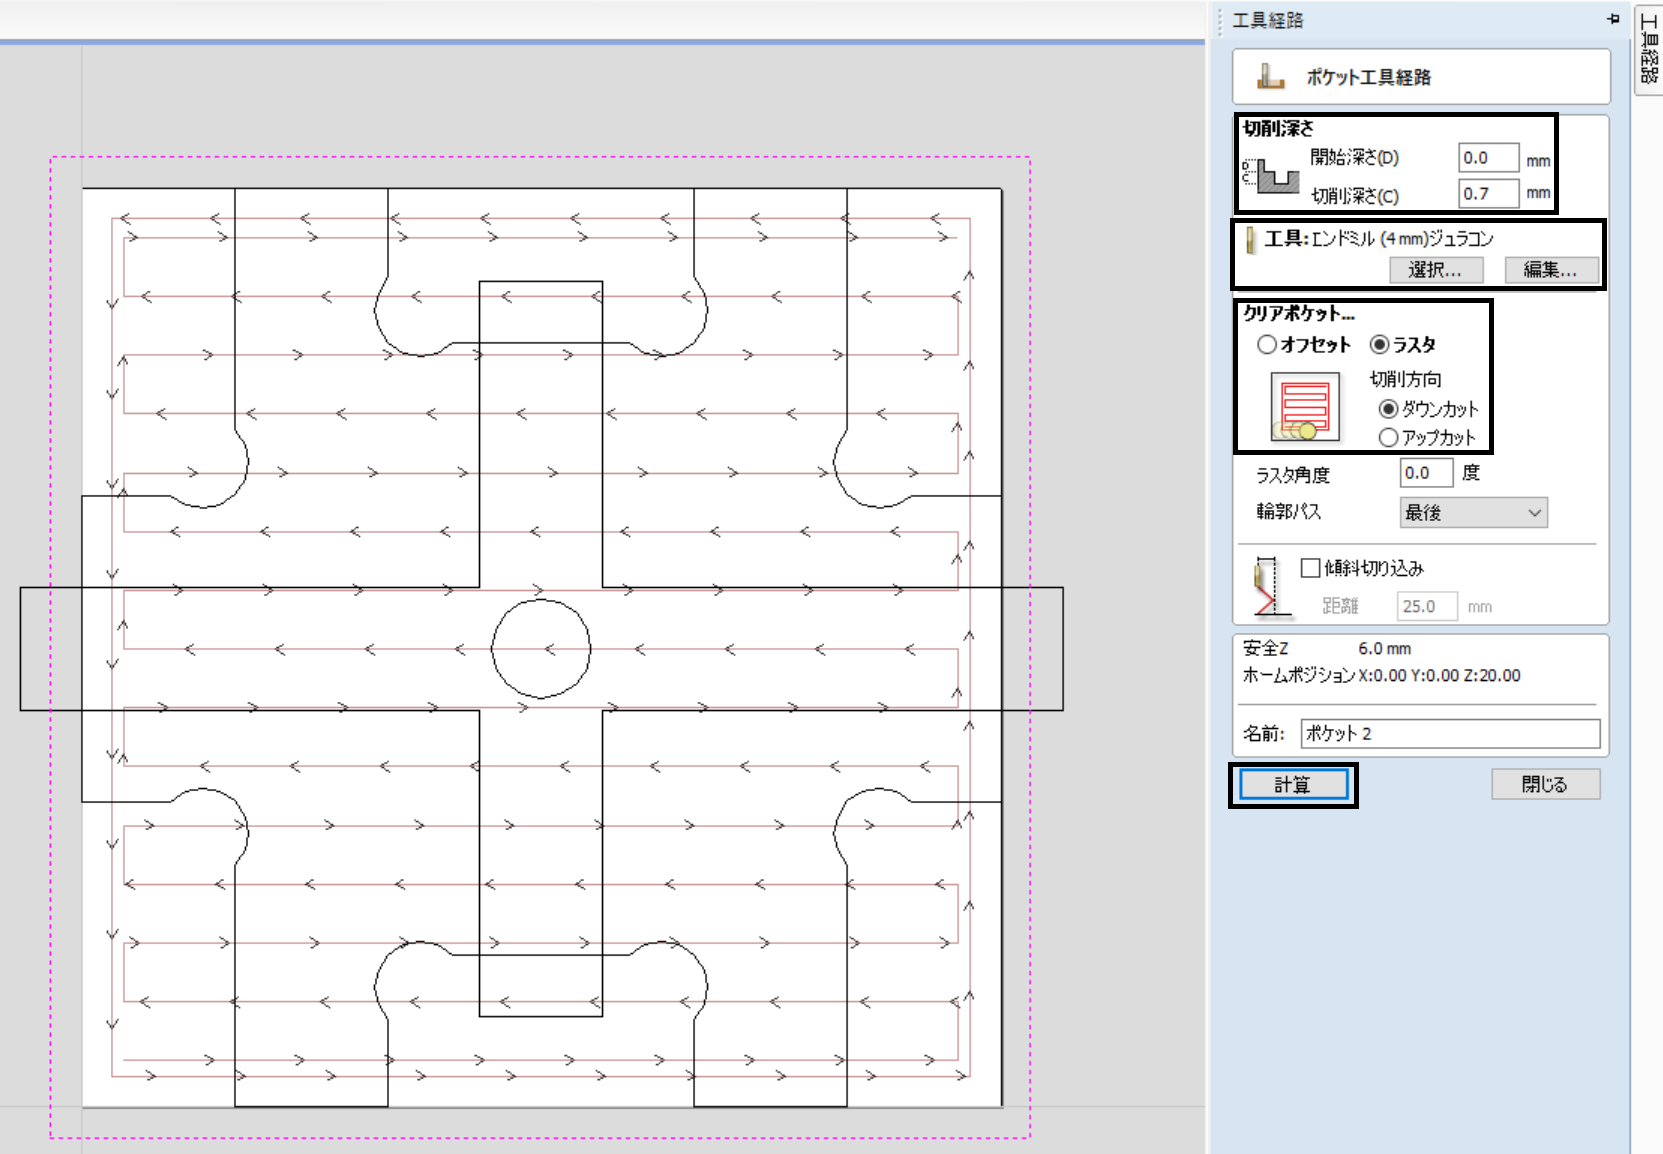
\includegraphics[width=\columnwidth]{pocket_milling_trim.png}
    \end{minipage}
    \caption{ポケット加工経路\label{pocket_milling}}
  \end{center}
\end{figure*}

%%画像*1 ポケット加工経路 pocket_milling_trim.png

\clearpage
次に経路の計算を行います。画面右上の工具経路ボタンを押して、工具経路タブを開きます。その後で、作る経路の種類を選択します。輪郭加工経路かポケット加工経路のボタンを押して図\ref{outer_milling}または図\ref{pocket_milling}の画面を開いた後に、使用するベクトルを選択し、次にパラメータの入力を行います。経路の計算のために入力するパラメータとしては、主に切削深さ、工具種類、切削方法(輪郭加工:外側・内側・中心 ポケット加工:オフセット・ラスタ)、切削方向(ダウンカット、アップカット)の4つがあります。切削深さについては、ノギスを用いて計測した厚みと自分の設計した部品の構造を考えて、各種経路の切削する深さを入力してください。ここで、前述のポケット加工を使って広い範囲を削ることで、厚みの精度を出すことが可能です。例えば、厚みの実測値が5.7mmの樹脂板の場合、0.7mmの深さのポケット加工を行うことで厚みを正確に5mmにすることができます。工具種類については、予め用意しておいた工具ファイルに含まれるもののうち、使用する工具の種類と速度に合わせたものを選んでください。工具ファイルはCNC環境と工具の種類に依存するので、分からない場合は使うCNCの管理者に聞いてください。切削方法は、前の段落を参照して決定してください。また、切削方向は、工具の寿命を考慮してダウンカットを選択してください。パラメータを入力したら、計算ボタンを押して経路を計算します。エラーが出なければ成功で、工具の中心が通る矢印線がベクトルの周りに表示されます。エラーが出た場合は、工具の径が加工したい幅より小さいことや、切削する深さが最初に設定した材料の厚みを超えていないことを確認してください。計算した工具経路は工具経路リストのウィンドウで一覧表示されています。経路の名前をクリックで選択、ダブルクリックでパラメータの設定画面を開く、横のチェック欄で表示非表示を切り替えることができます。これを繰り返し、最終的に図\ref{milling_vector}のような経路になります。\\

\begin{figure*}[tbh]
  \begin{center}
    \begin{minipage}{0.9\columnwidth}
      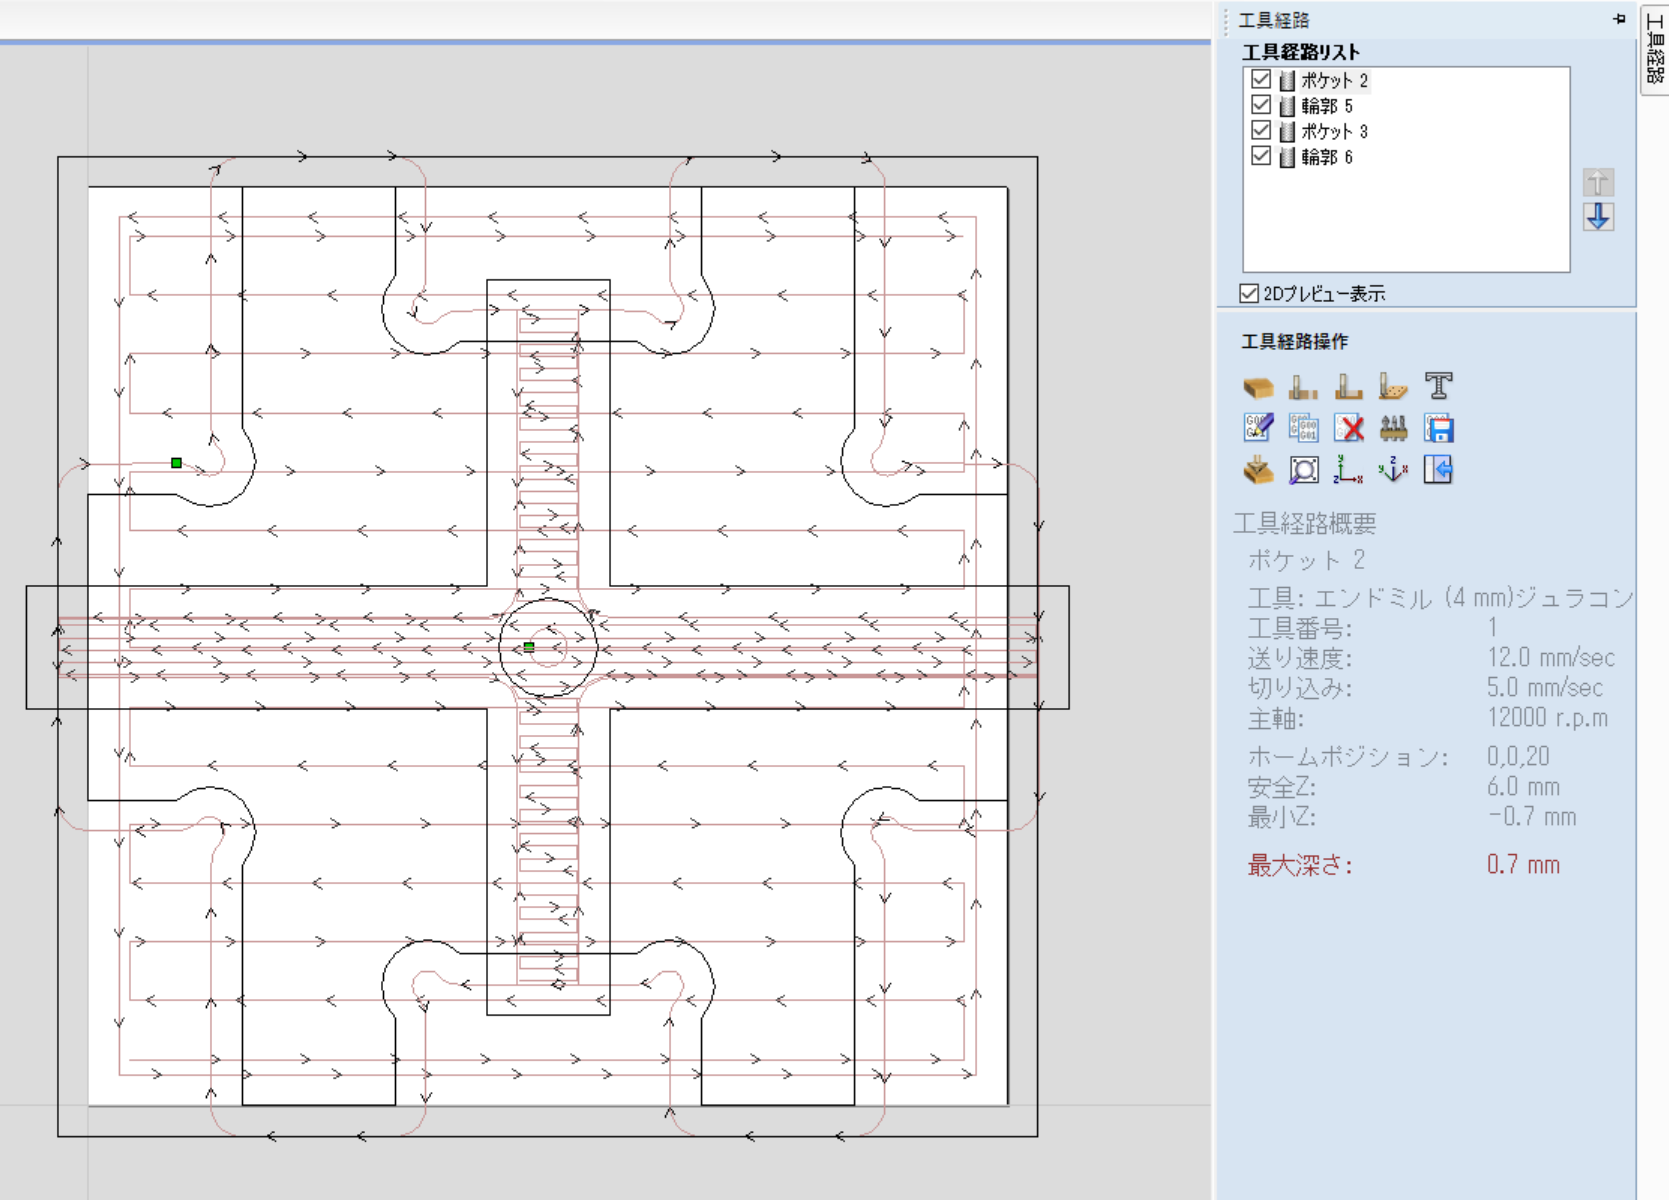
\includegraphics[width=\columnwidth]{milling_vector_trim.png}
    \end{minipage}
    \caption{最終的な経路    \label{milling_vector}}
  \end{center}
\end{figure*}

%%  画像*1 最終的な切削経路 milling_vector_trim.png

\clearpage
工具経路を一通り作ったら、作った経路の整理をします。不要な工具経路を選択した後に、工具経路タブの工具経路削除ボタンを押すと削除が可能です。必要な経路だけになったら、加工する順番に応じて経路の順番を並べ替えます。経路を選択した上で工具経路リストウィンドウ横の上下矢印ボタンを押すことで順番を並べ変えられます。この順番は行いたい加工によっても異なるのですが、基本的には外側輪郭加工を最後に行うことをお勧めします。先に外側を切り抜いてしまうと、両面テープによる固定力が低くなり、内側に穴をあける時に材料がずれやすくなるため、外側の切り抜きを最後に行うことでこのミスを防ぎやすくなります。\\

次に、整理した加工経路のプレビューを行います。工具経路タブの工具経路プレビューボタンを押して、図\ref{preview}の画面を開きます。経路を単体でプレビューする場合は工具経路プレビューボタン、すべての経路をプレビューする場合は全工具プレビューボタンを押します。プレビューが始まると、工具が材料を切削していくアニメーションが流れ、切削の様子を三次元的に表示してくれます。どのように切削されるのかを確認できるため、間違っている場合に修正を行うことができます。プレビューが終わった後にはマウス左クリックドラッグで回転もできます。プレビューが長くて途中で止めたい場合には、図\ref{preview_stop}のようにプレビューの下に表示されている進行度を示すバーの横にあるXボタンを押してください。また、プレビュー画面とベクトル表示画面は、プレビュー画面左上にあるタブで切り替えが可能です。経路を作成、プレビューで確認、経路を修正 という流れを繰り返して、自分の思った通りの経路になったら、経路の作成は終了です。\\
\begin{figure*}[tbh]
  \begin{center}
    \begin{minipage}{0.6\columnwidth}
      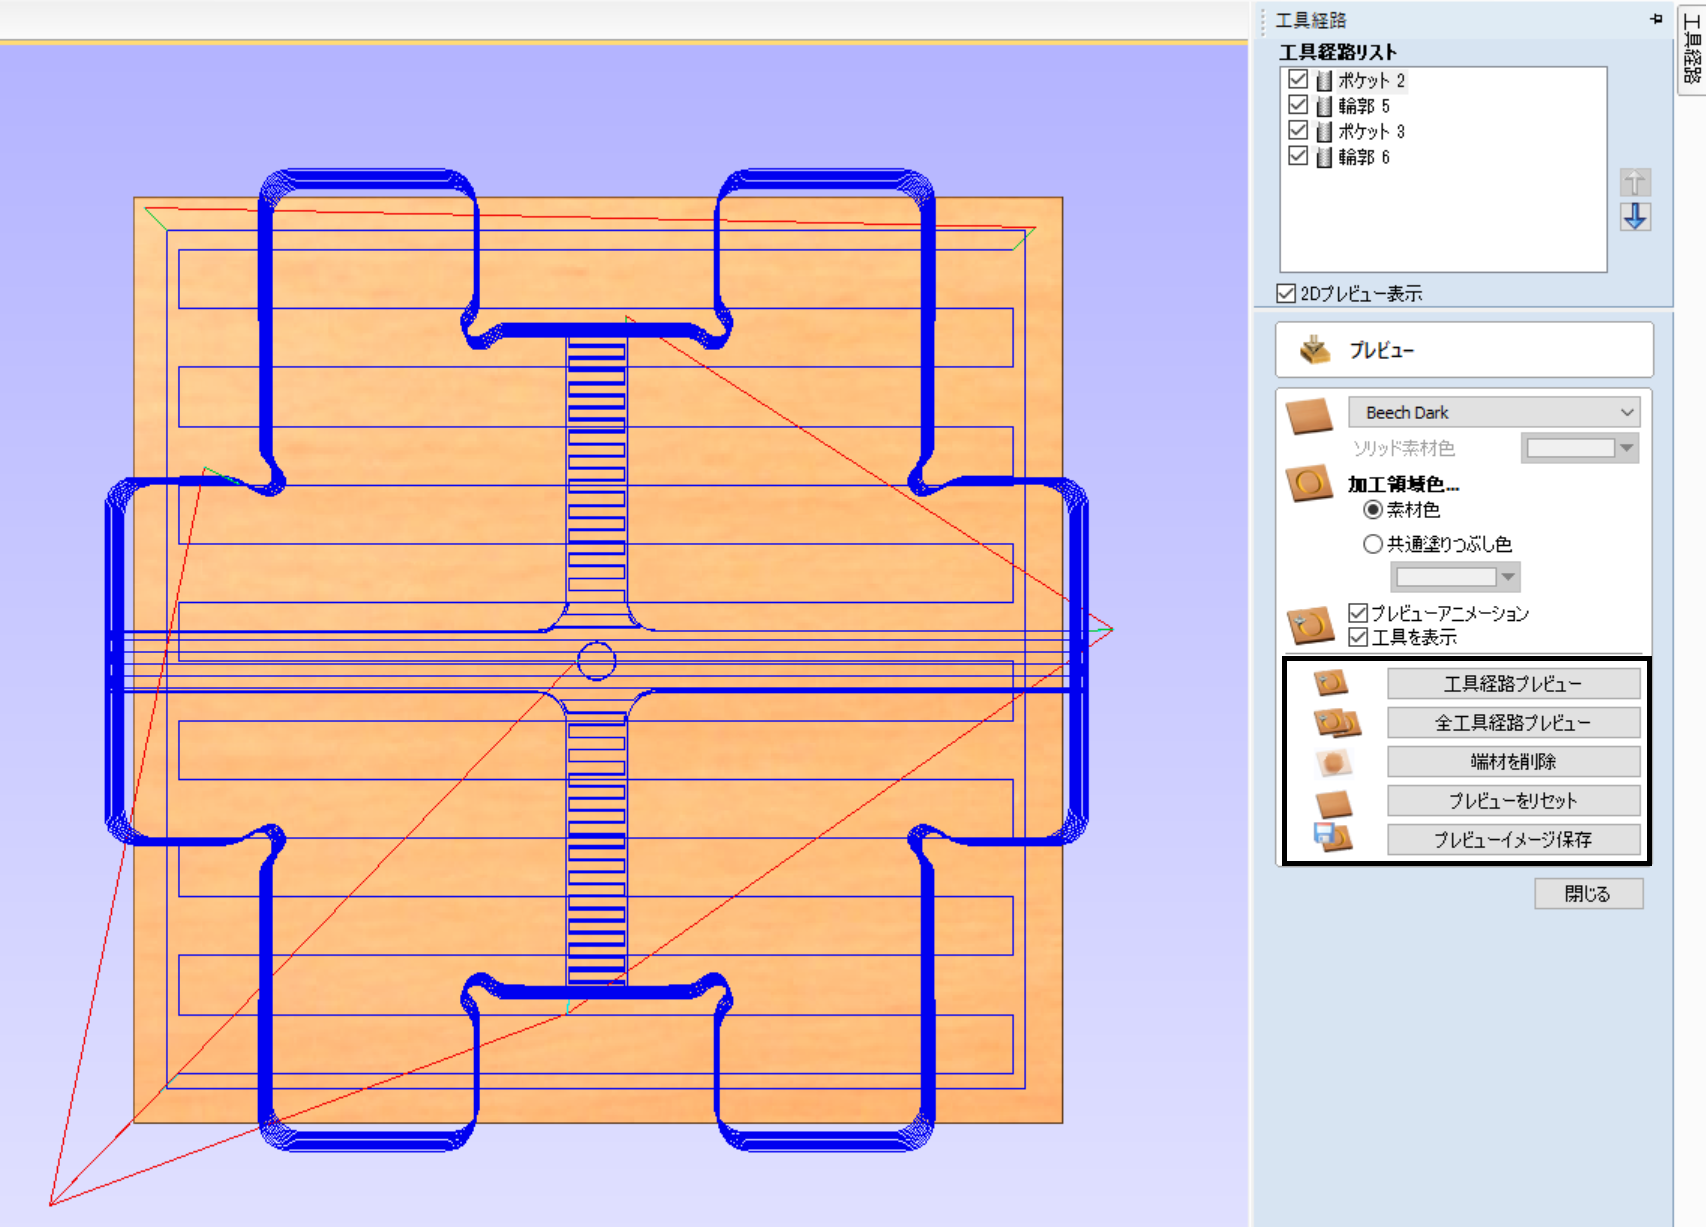
\includegraphics[width=\columnwidth]{preview_trim.png}
    \end{minipage}
    \begin{minipage}{0.3\columnwidth}
      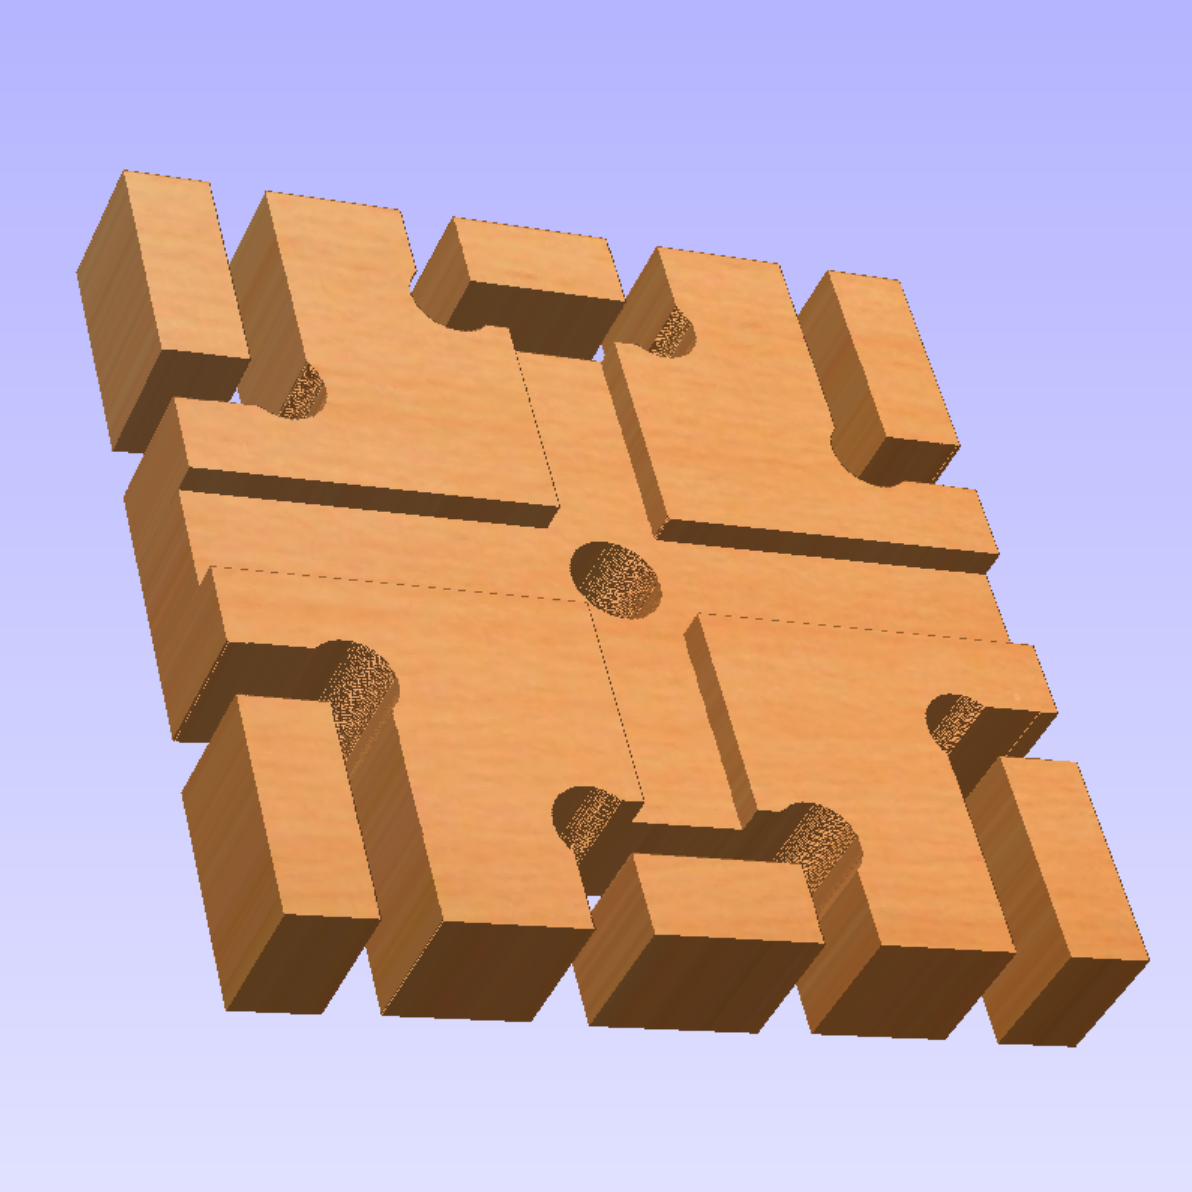
\includegraphics[width=\columnwidth]{preview_isome_trim.png}
    \end{minipage}
    \caption{工具経路プレビュー}
    \begin{minipage}{1.0\columnwidth    \label{preview}}
      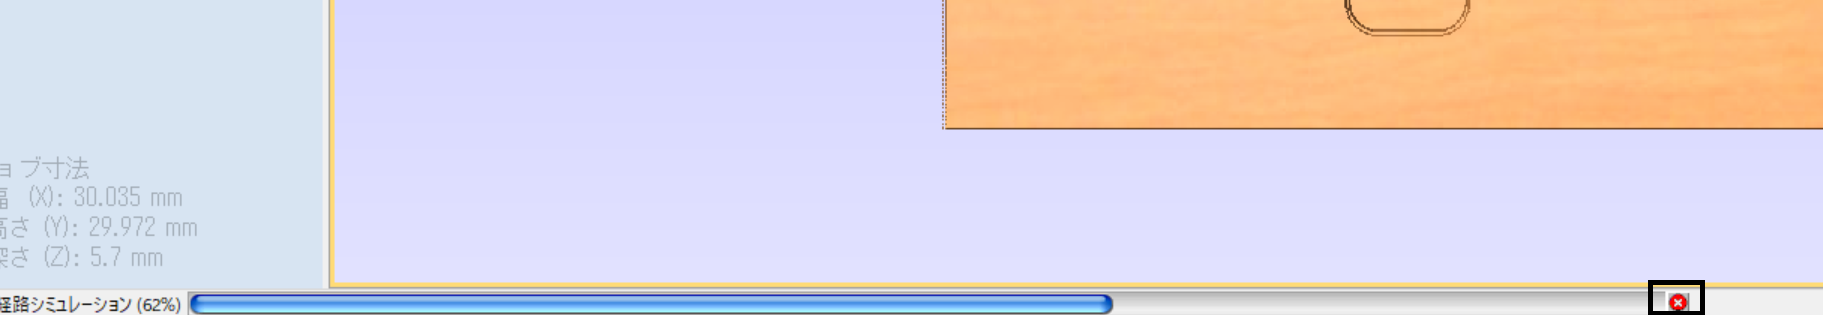
\includegraphics[width=\columnwidth]{preview_now_trim.png}
    \end{minipage}
    \caption{プレビュー停止    \label{preview_stop}}
  \end{center}
\end{figure*}

%% \begin{figure*}[tbh]
%%   \begin{center}
%%     \begin{minipage}{0.8\columnwidth}
%%       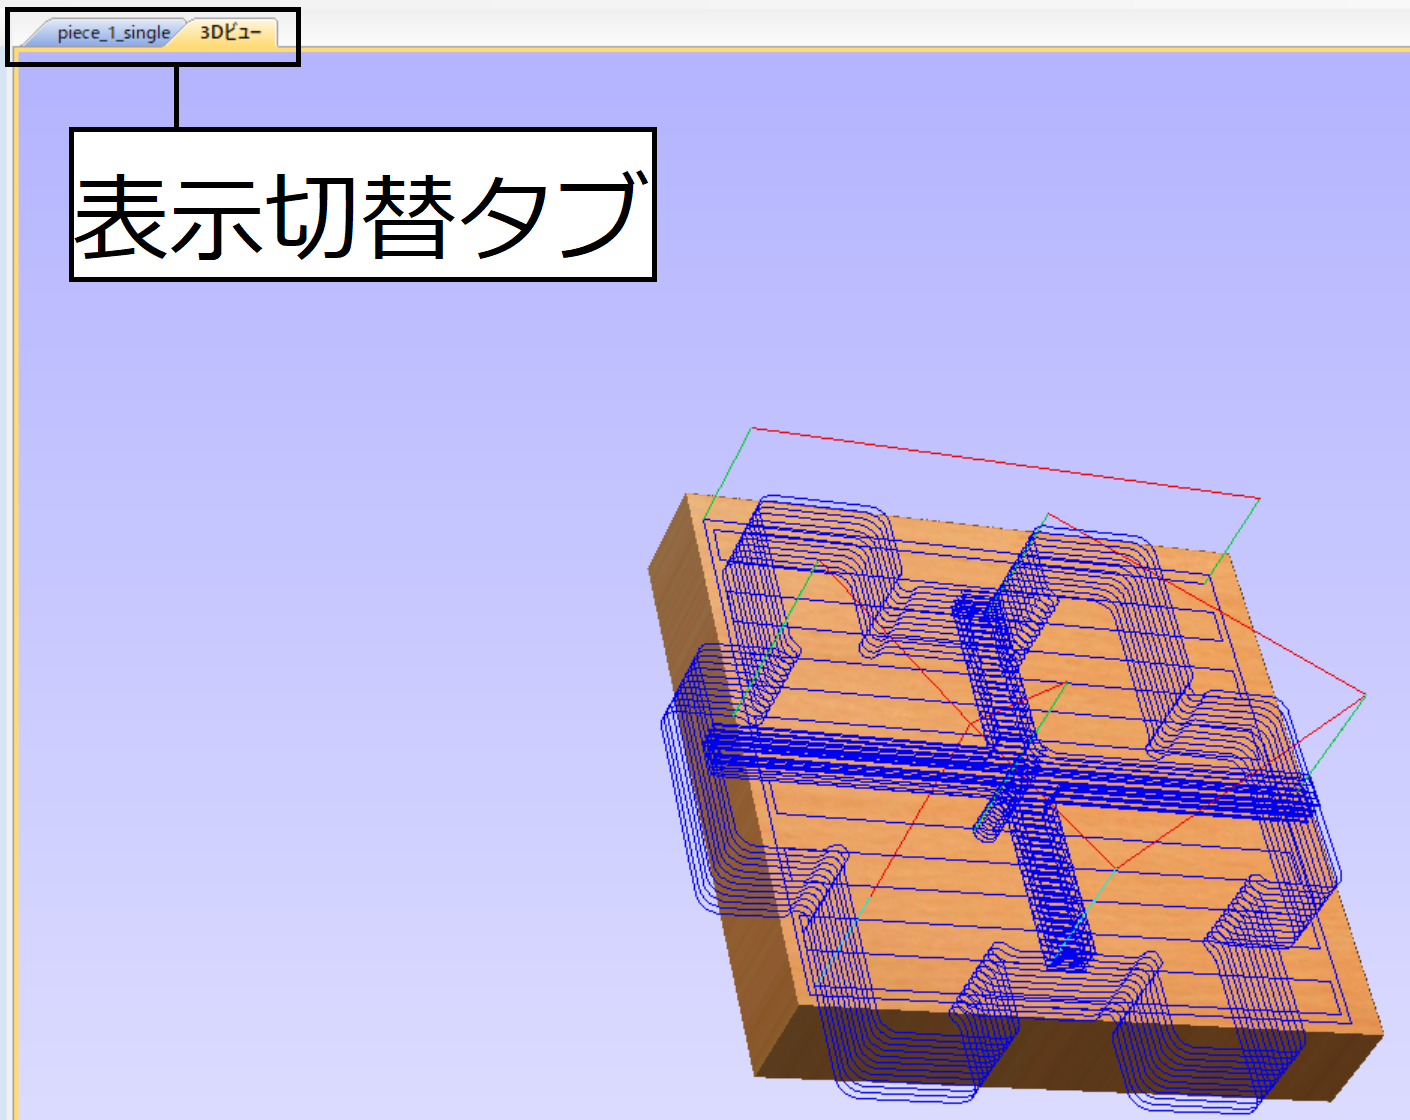
\includegraphics[width=\columnwidth]{milling_tab_trim2.png}
%%     \end{minipage}
%%     \caption{表示切り替え    \label{preview_tab}}
%%   \end{center}
%% \end{figure*}

%%画像*4 経路プレビュー、アニメーション preview_trim.png preview_isome_trim.png preview_now_trim.png milling_tab_trim2.png

\clearpage
\subsection{加工ファイル出力}

最後に、作成した経路をNCファイルとして出力します。使用している工具の径がすべて同じ場合、工具経路リストの☑欄を全て入れ、全可視工具経路を1ファイルに出力 の☑を入れ、ポストプロセッサを選択(今回はUSBCNC)した後に具経路保存ボタンを押すことでNCファイルを出力できます。ここでは☑を入れた工具経路だけがNCファイルに出力されるため、必要な経路にだけ☑を付けてください。一方、工具経路によって工具の径が異なる場合、図\ref{fail}のような赤文字のエラーが出るので、工具の径が異なる経路の☑を外して、図\ref{succeed}のように工具の径ごとにNCファイルを出力する必要があります。この場合、後の工程3での加工の途中にエンドミルを取り換える必要があります。使用したい全ての経路をNCファイルで出力したらこの工程は終了です。\\

\begin{figure*}[tbh]
  \begin{center}
    \begin{minipage}{0.6\columnwidth}
      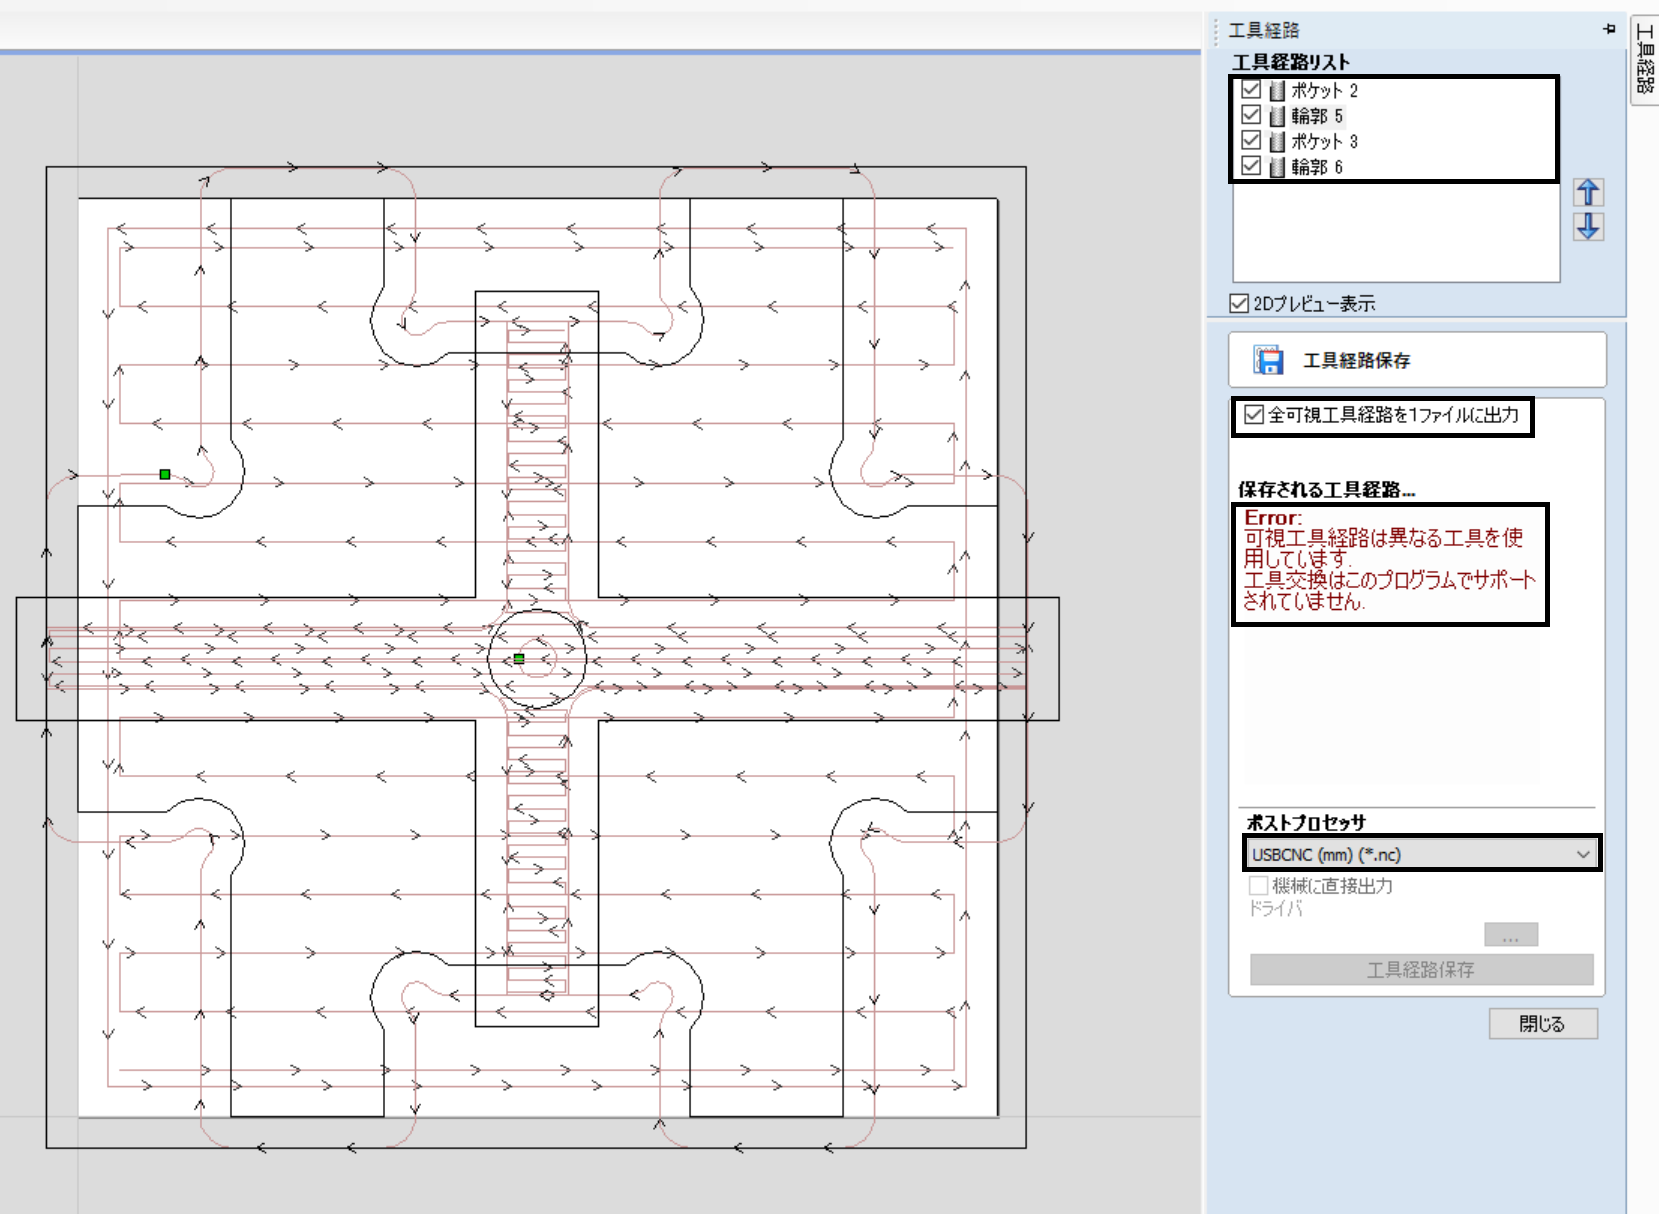
\includegraphics[width=\columnwidth]{NC_output_fail_trim.png}
    \end{minipage}
    \caption{出力不可能\label{fail}}
    \begin{minipage}{0.6\columnwidth}
      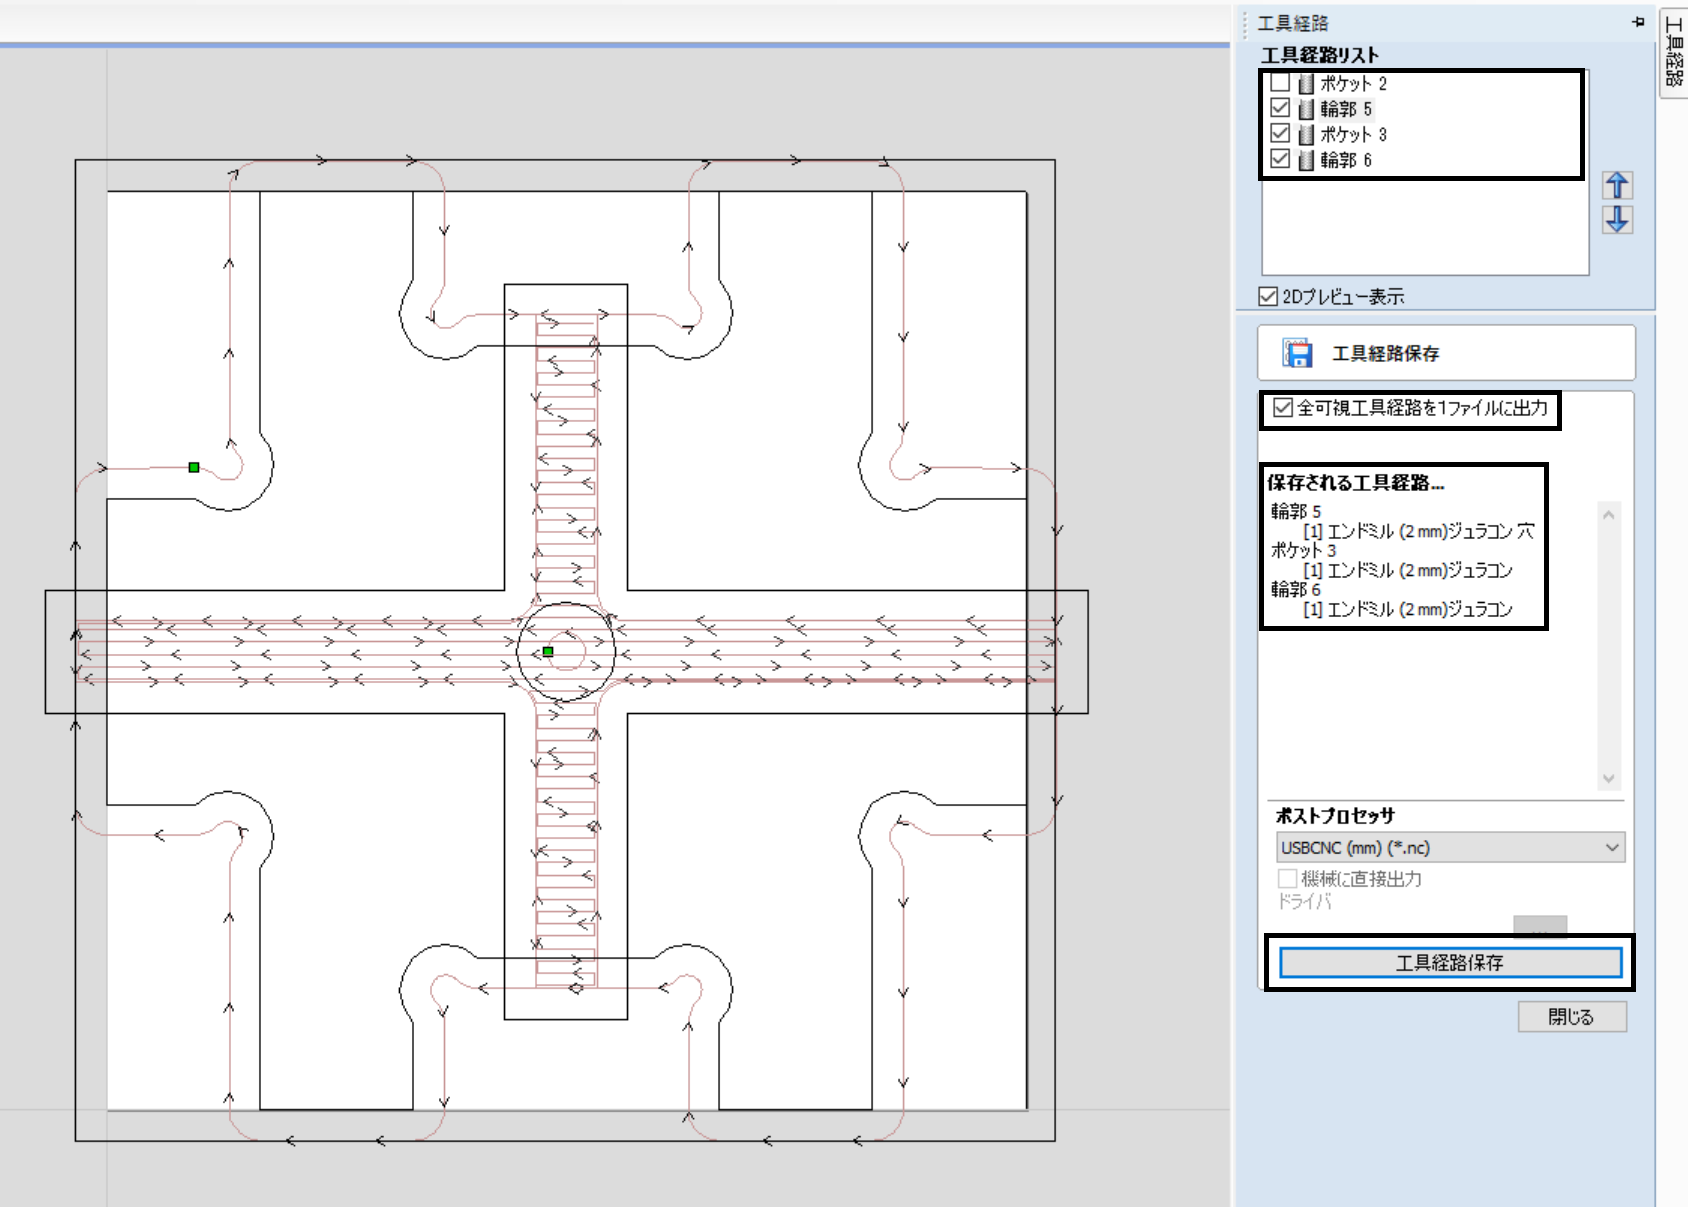
\includegraphics[width=\columnwidth]{NC_output_succeed_trim.png}
    \end{minipage}
    \caption{出力可能\label{succeed}}
  \end{center}
\end{figure*}

%%画像*2 失敗、成功 NC_output_fail_trim.png NC_output_succeed_trim.png



\clearpage
\section{工程3.CNC(RD300,USBCNC)での作業、清掃}
ここでは、実際のCNCでの作業を順を追って説明します。基本的な流れとしては、\\
  1.材料の固定(RD420)\\
  2.エンドミルの清掃・固定(RD420)\\
  3.NCファイルの読み込み(USBCNC)\\
  4.原点合わせ(RD420,USBCNC)\\
  5.加工(RD420,USBCNC)\\
  6.清掃(RD420)\\
  7.仕上げ\\
  という順番で行います。今回はOriginalMindのRD300を使いますが、違う環境の場合は各自読み替えて下さい。\\

\subsection{材料の固定}
まず、材料の固定を行います。今回はoriginalmindのRD420(図\ref{RD420})を用いて説明を行うため、図\ref{kotei}のように両面テープを用いて固定を行います。また、今回はPOMの板を材料として加工しています。当然ですが、材料は加工したいパーツより大きく、CNCに収まるサイズのものを用意してください。CNCに固定されている捨て板に両面テープを張った後に剥離紙を剥がして材料を張り付けます。ここで気をつけることとしては、両面テープを張る前に十分に捨て板を清掃することです。前回の加工の際に出た切りくずや、切削のための潤滑油がそのまま残っていると、両面テープと捨て板・材料の間に隙間ができて加工中に材料がはがれやすくなってしまいます。一度はがれてしまうと、元の場所に固定しなおすことは基本的にできないため、剥がれないようにしっかりと固定しましょう。\\

\begin{figure*}[tbh]
  \begin{center}
    \begin{minipage}{1.0\columnwidth}
      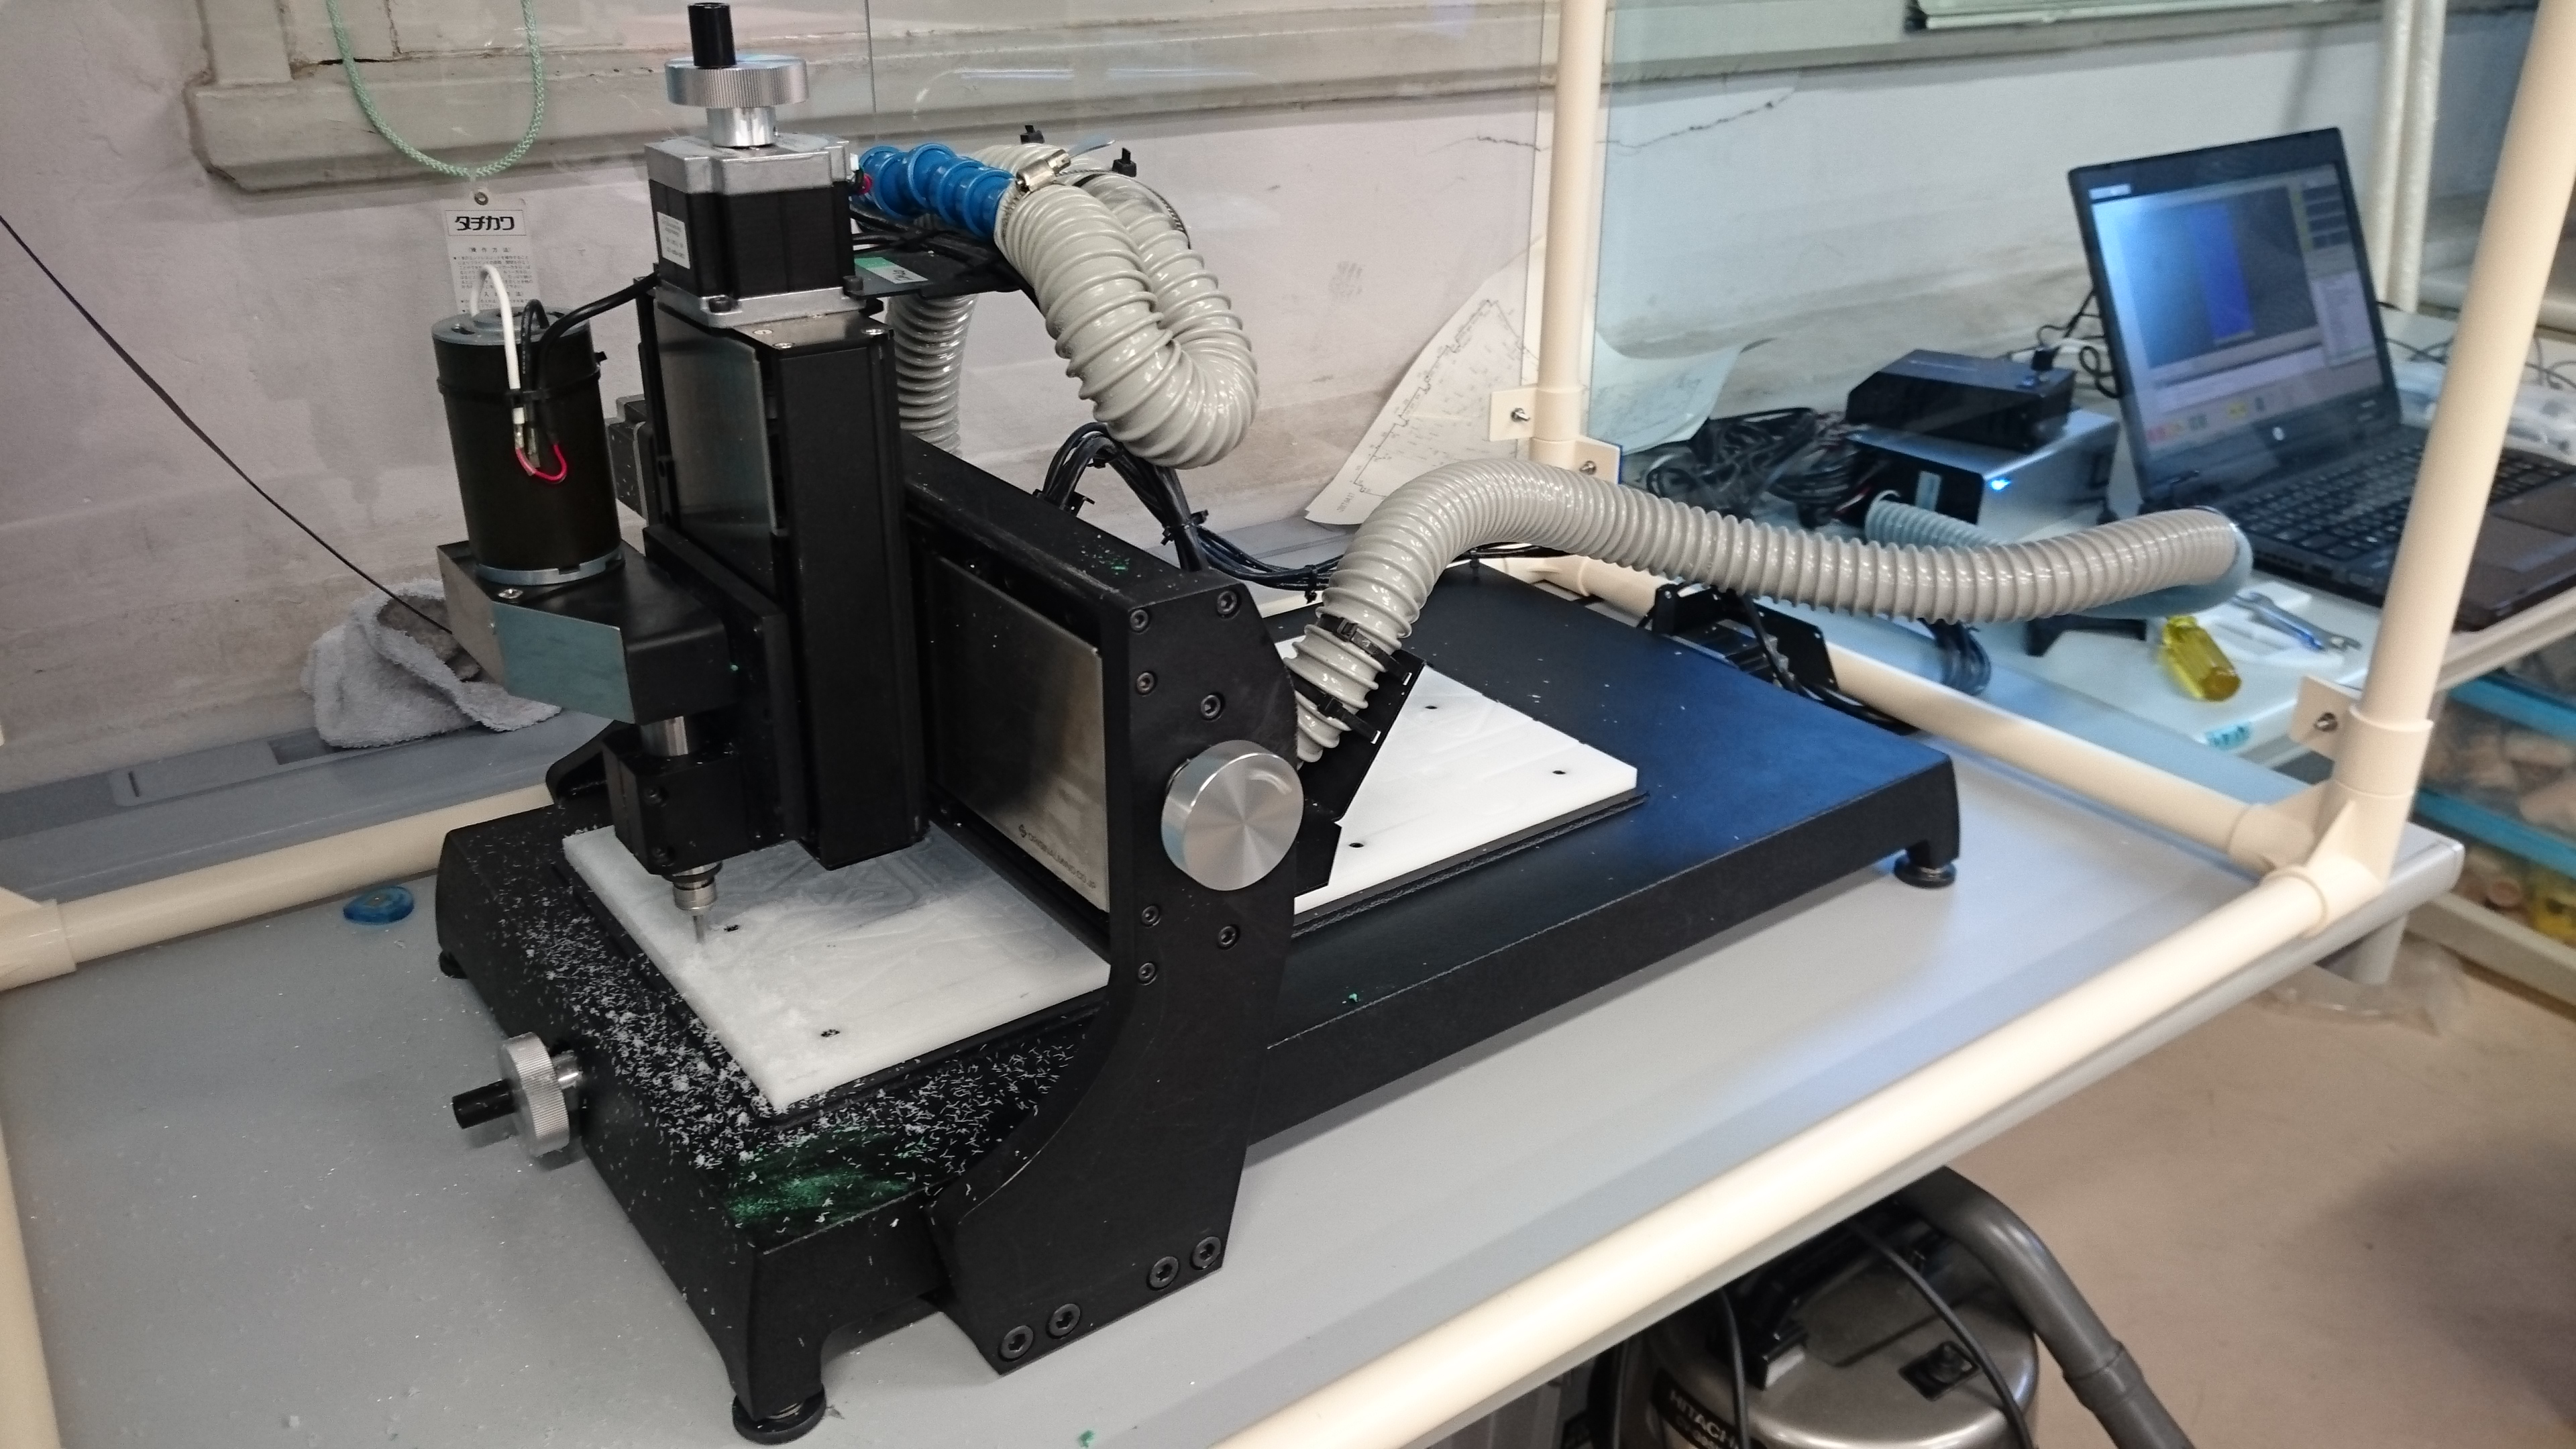
\includegraphics[width=\columnwidth]{RD420.jpg}
    \end{minipage}
    \caption{今回使うCNC\label{RD420}}
    \begin{minipage}{1.0\columnwidth}
      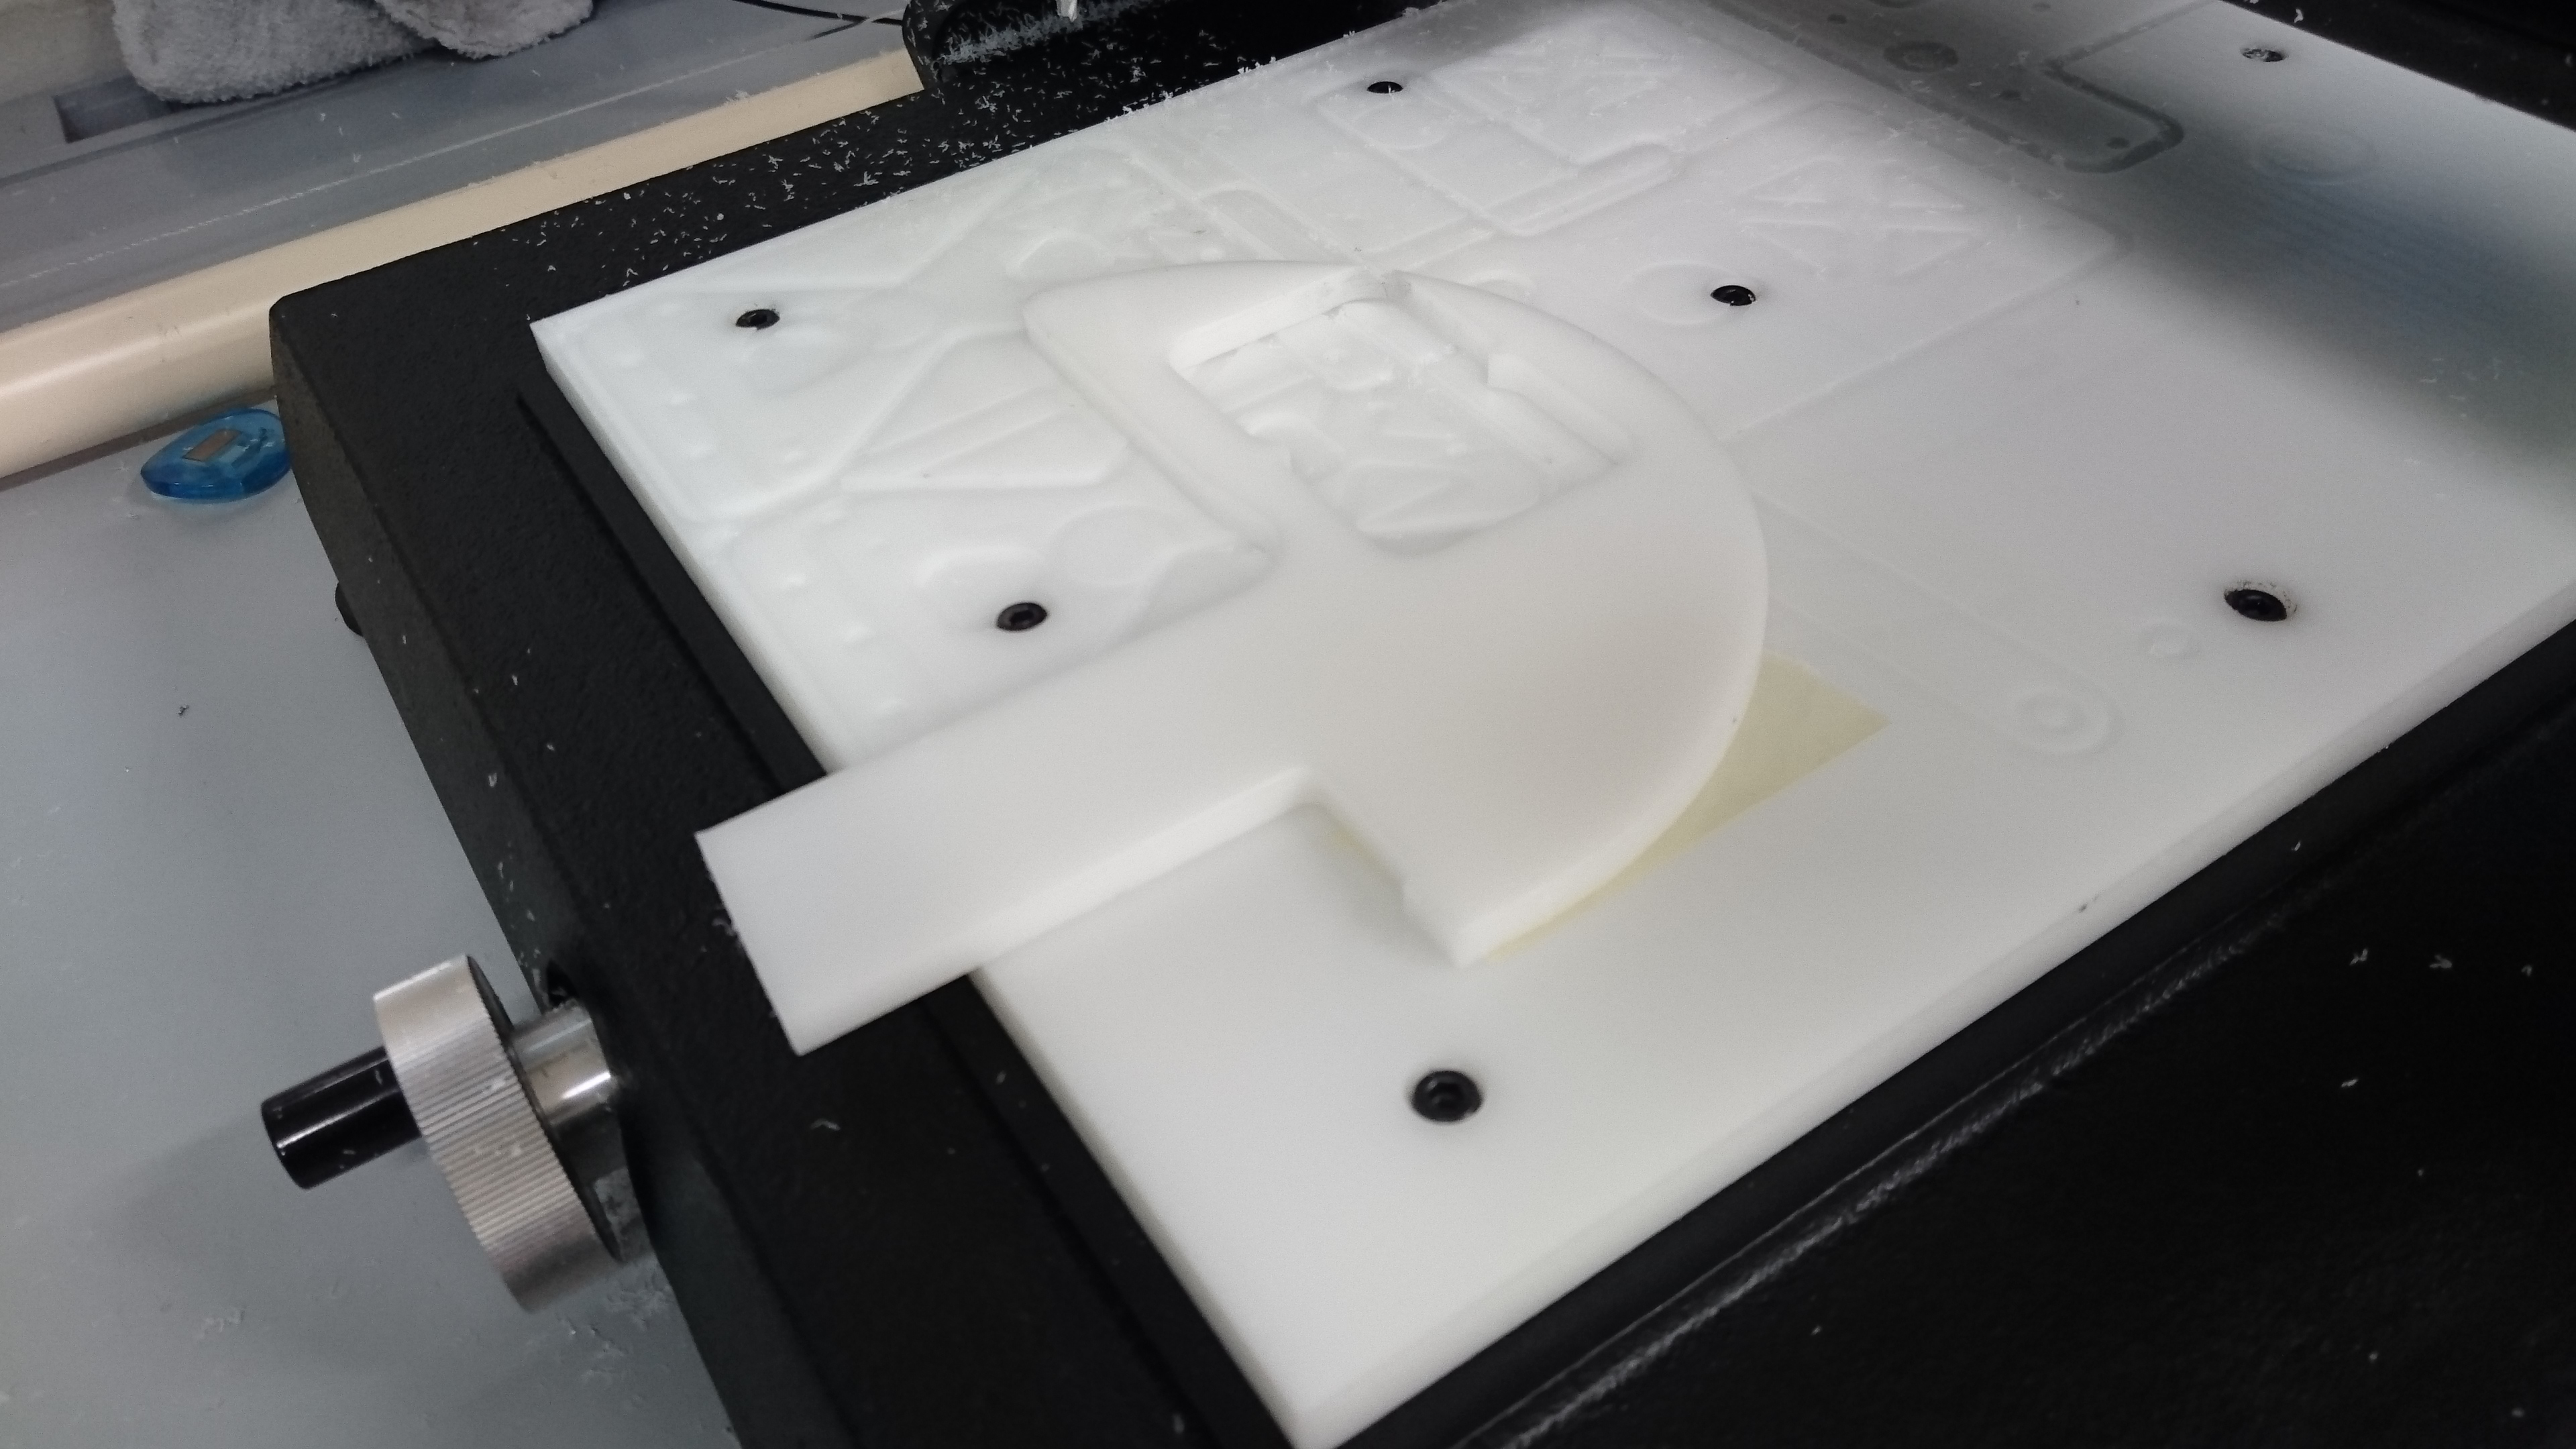
\includegraphics[width=\columnwidth]{kotei.jpg}
    \end{minipage}
    \caption{樹脂板の貼り付け\label{kotei}}
  \end{center}
\end{figure*}

%画像*2 RD420、材を固定した画像 RD420.jpg kotei.jpg

\clearpage
\subsection{ファイルの読み込み、CNCとの接続}
次に、USBCNCとRD420との接続を行います。RD420の電源を入れ、USBCNCを立ち上げ、出てきた画面でresetボタン(画面下の赤いボタン)を押します。矢印キーを少し押して、RD420のエンドミル位置が動いたら接続成功です。次に、CNCでNCファイルの読み込みを行います。図\ref{file_open}に従って操作をして、使用するNCファイルの選択を行ってください。今回作ったNCファイルの拡張子は.ncです。ファイルを読み込むと、図\ref{after_open}のように加工の目安時間が出ます。\\

\begin{figure*}[tbh]
  \begin{center}
    \begin{minipage}{0.8\columnwidth}
      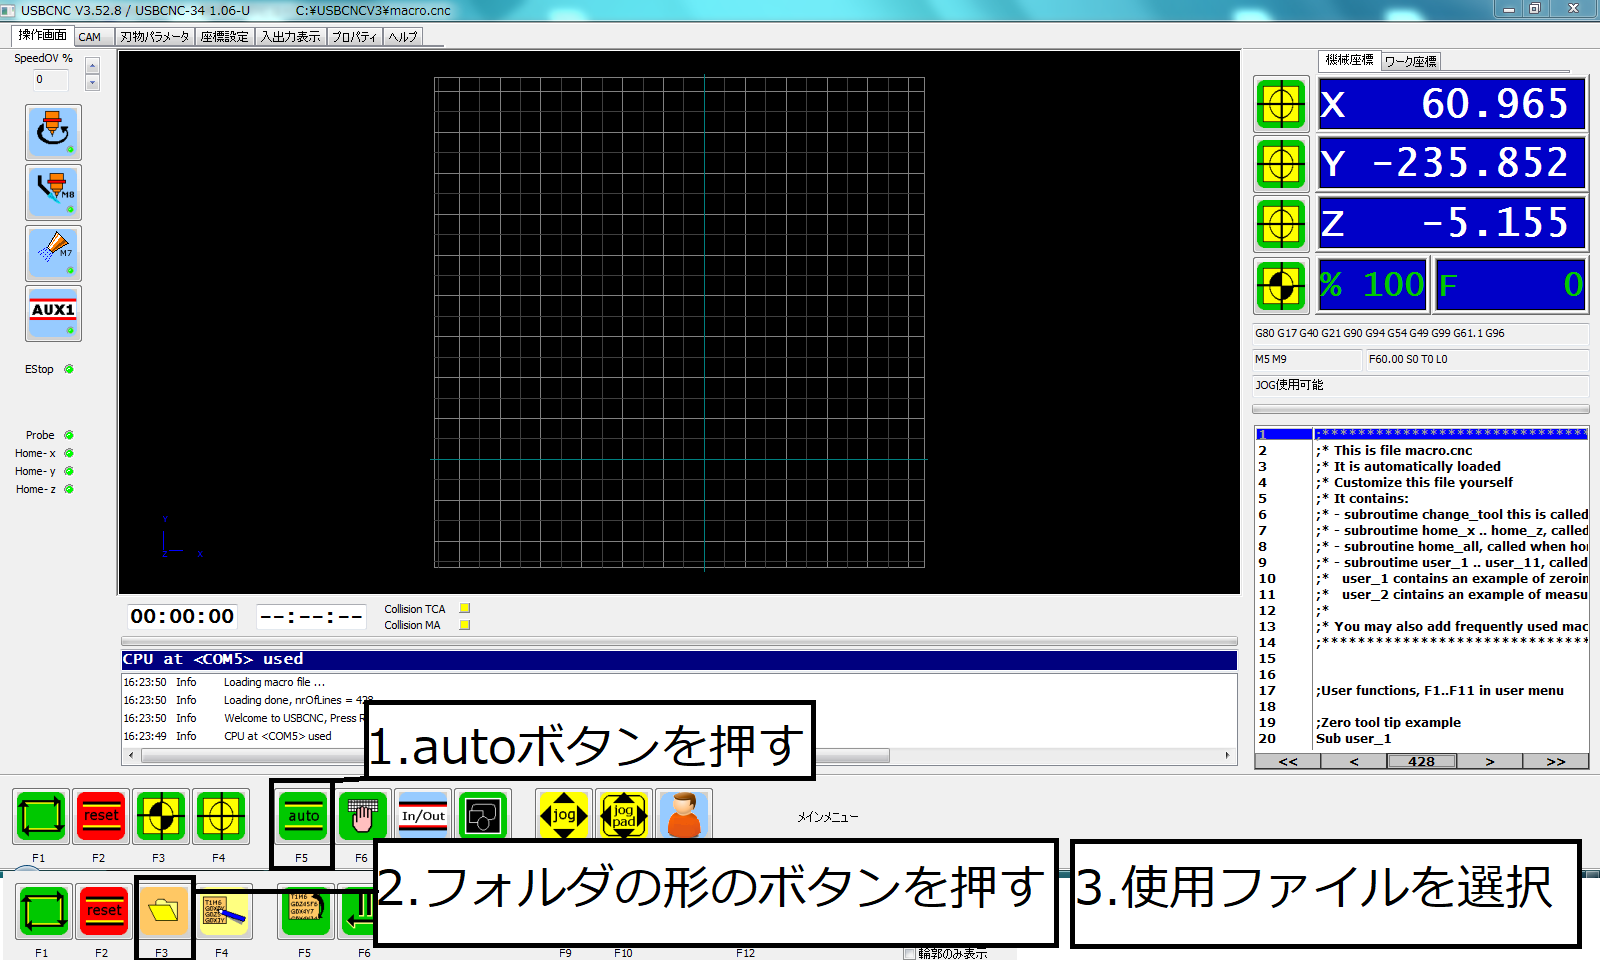
\includegraphics[width=\columnwidth]{file_open.png}
    \end{minipage}
    \caption{NCファイルの読み込み\label{file_open}}
    \begin{minipage}{0.8\columnwidth}
      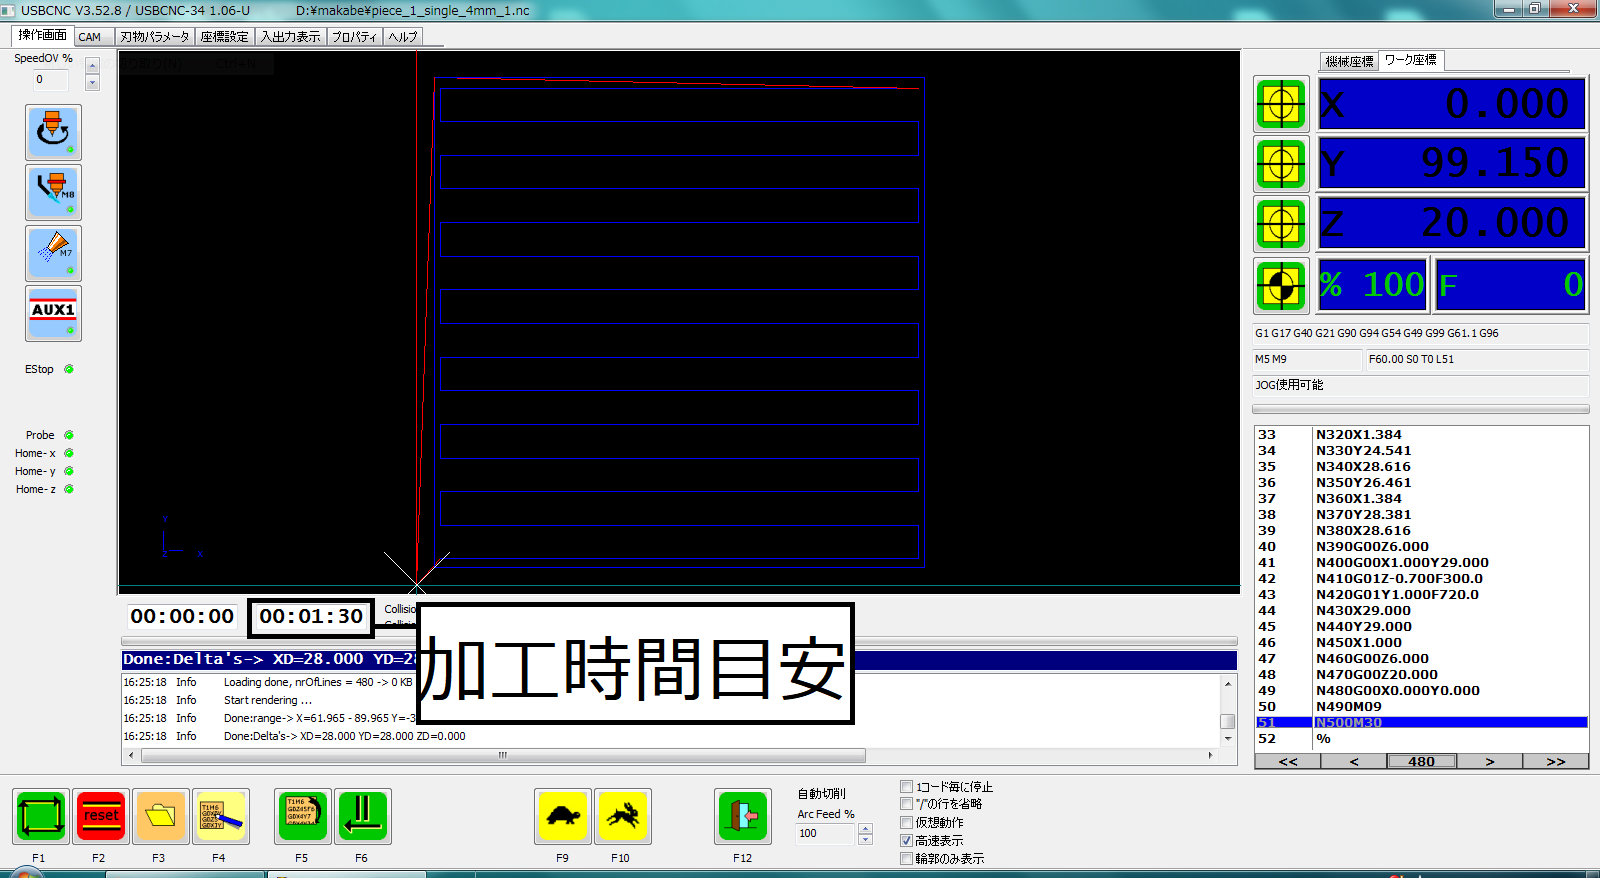
\includegraphics[width=\columnwidth]{file_open_after2.png}
    \end{minipage}
    \caption{加工時間の目安\label{after_open}}
  \end{center}
\end{figure*}

%%画像*2 ファイル読み込み 加工ファイル file_open.png file_open_after2.png

\clearpage
\subsection{エンドミルの清掃・固定}
エンドミルを固定する前に、エンドミルの清掃を行います。前の加工の時の両面テープのくずなどが残っている場合があるので、パーツクリーナーなどを使って清掃を行います。清掃が不十分だと、原点合わせの際にエンドミルを材料に押し付けきれず原点がずれてしまうので、気をつけて下さい。図\ref{endmill_4mm}にある程度綺麗であれば問題ありません。次にエンドミルをしっかりと固定します。エンドミルの固定方法としてはいくつかありますが、ここではコレットでの固定になります。スピンドルを一旦Z軸方向にあげた後にエンドミルを穴に差し込んで、コレット押し付けねじを軽く締めて仮止めをしてください。ここでは、エンドミルが下に落ちない程度に軽く止まっていれば大丈夫です。次に、スピンドルのZ軸を下げつつ、図\ref{push}のようにエンドミルを材料に押し付けます。その次に一度ネジを緩めることで、エンドミルは自重で材料に押し付けられます。ここで改めてネジを締めて、エンドミルの本止めをします。ここでの固定が微妙だと、加工している最中にエンドミルがスピンドルの方向に押し込まれて削り残しができてしまうので、気をつけて固定して下さい。本止めができたら、原点合わせをするまでエンドミルを動かさないで下さい。\\

\begin{figure*}[tbh]
  \begin{center}
    \begin{minipage}{0.7\columnwidth}
      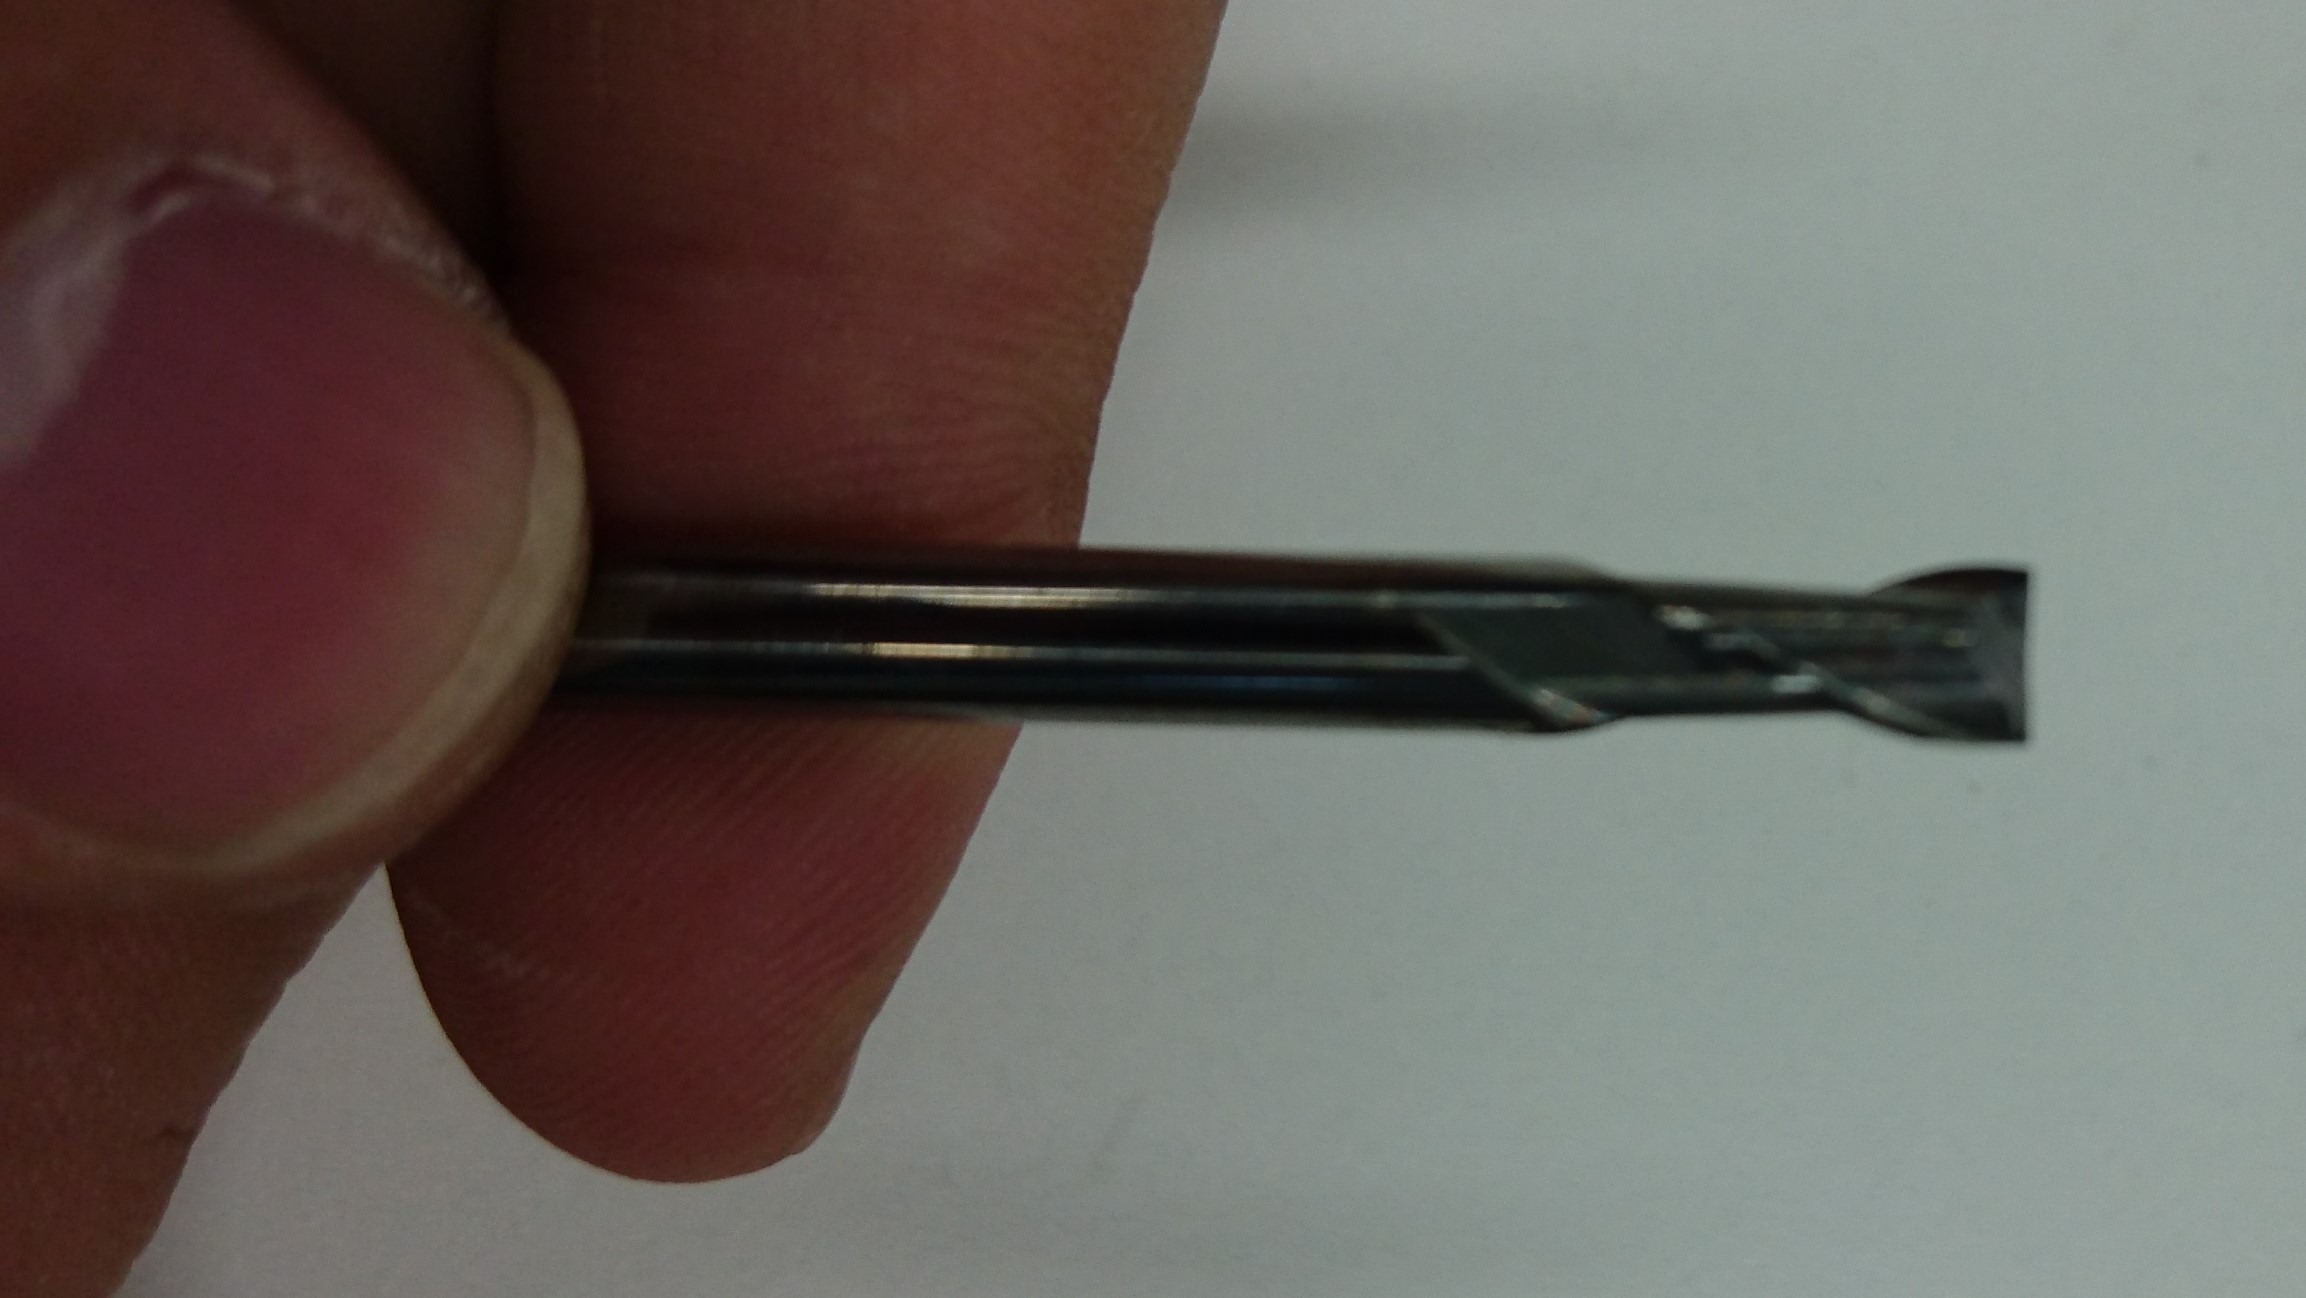
\includegraphics[width=\columnwidth]{endmill_4mm_side.jpg}
    \end{minipage}
    \caption{エンドミル(Φ4mm\label{endmill_4mm})}
    \begin{minipage}{0.7\columnwidth}
      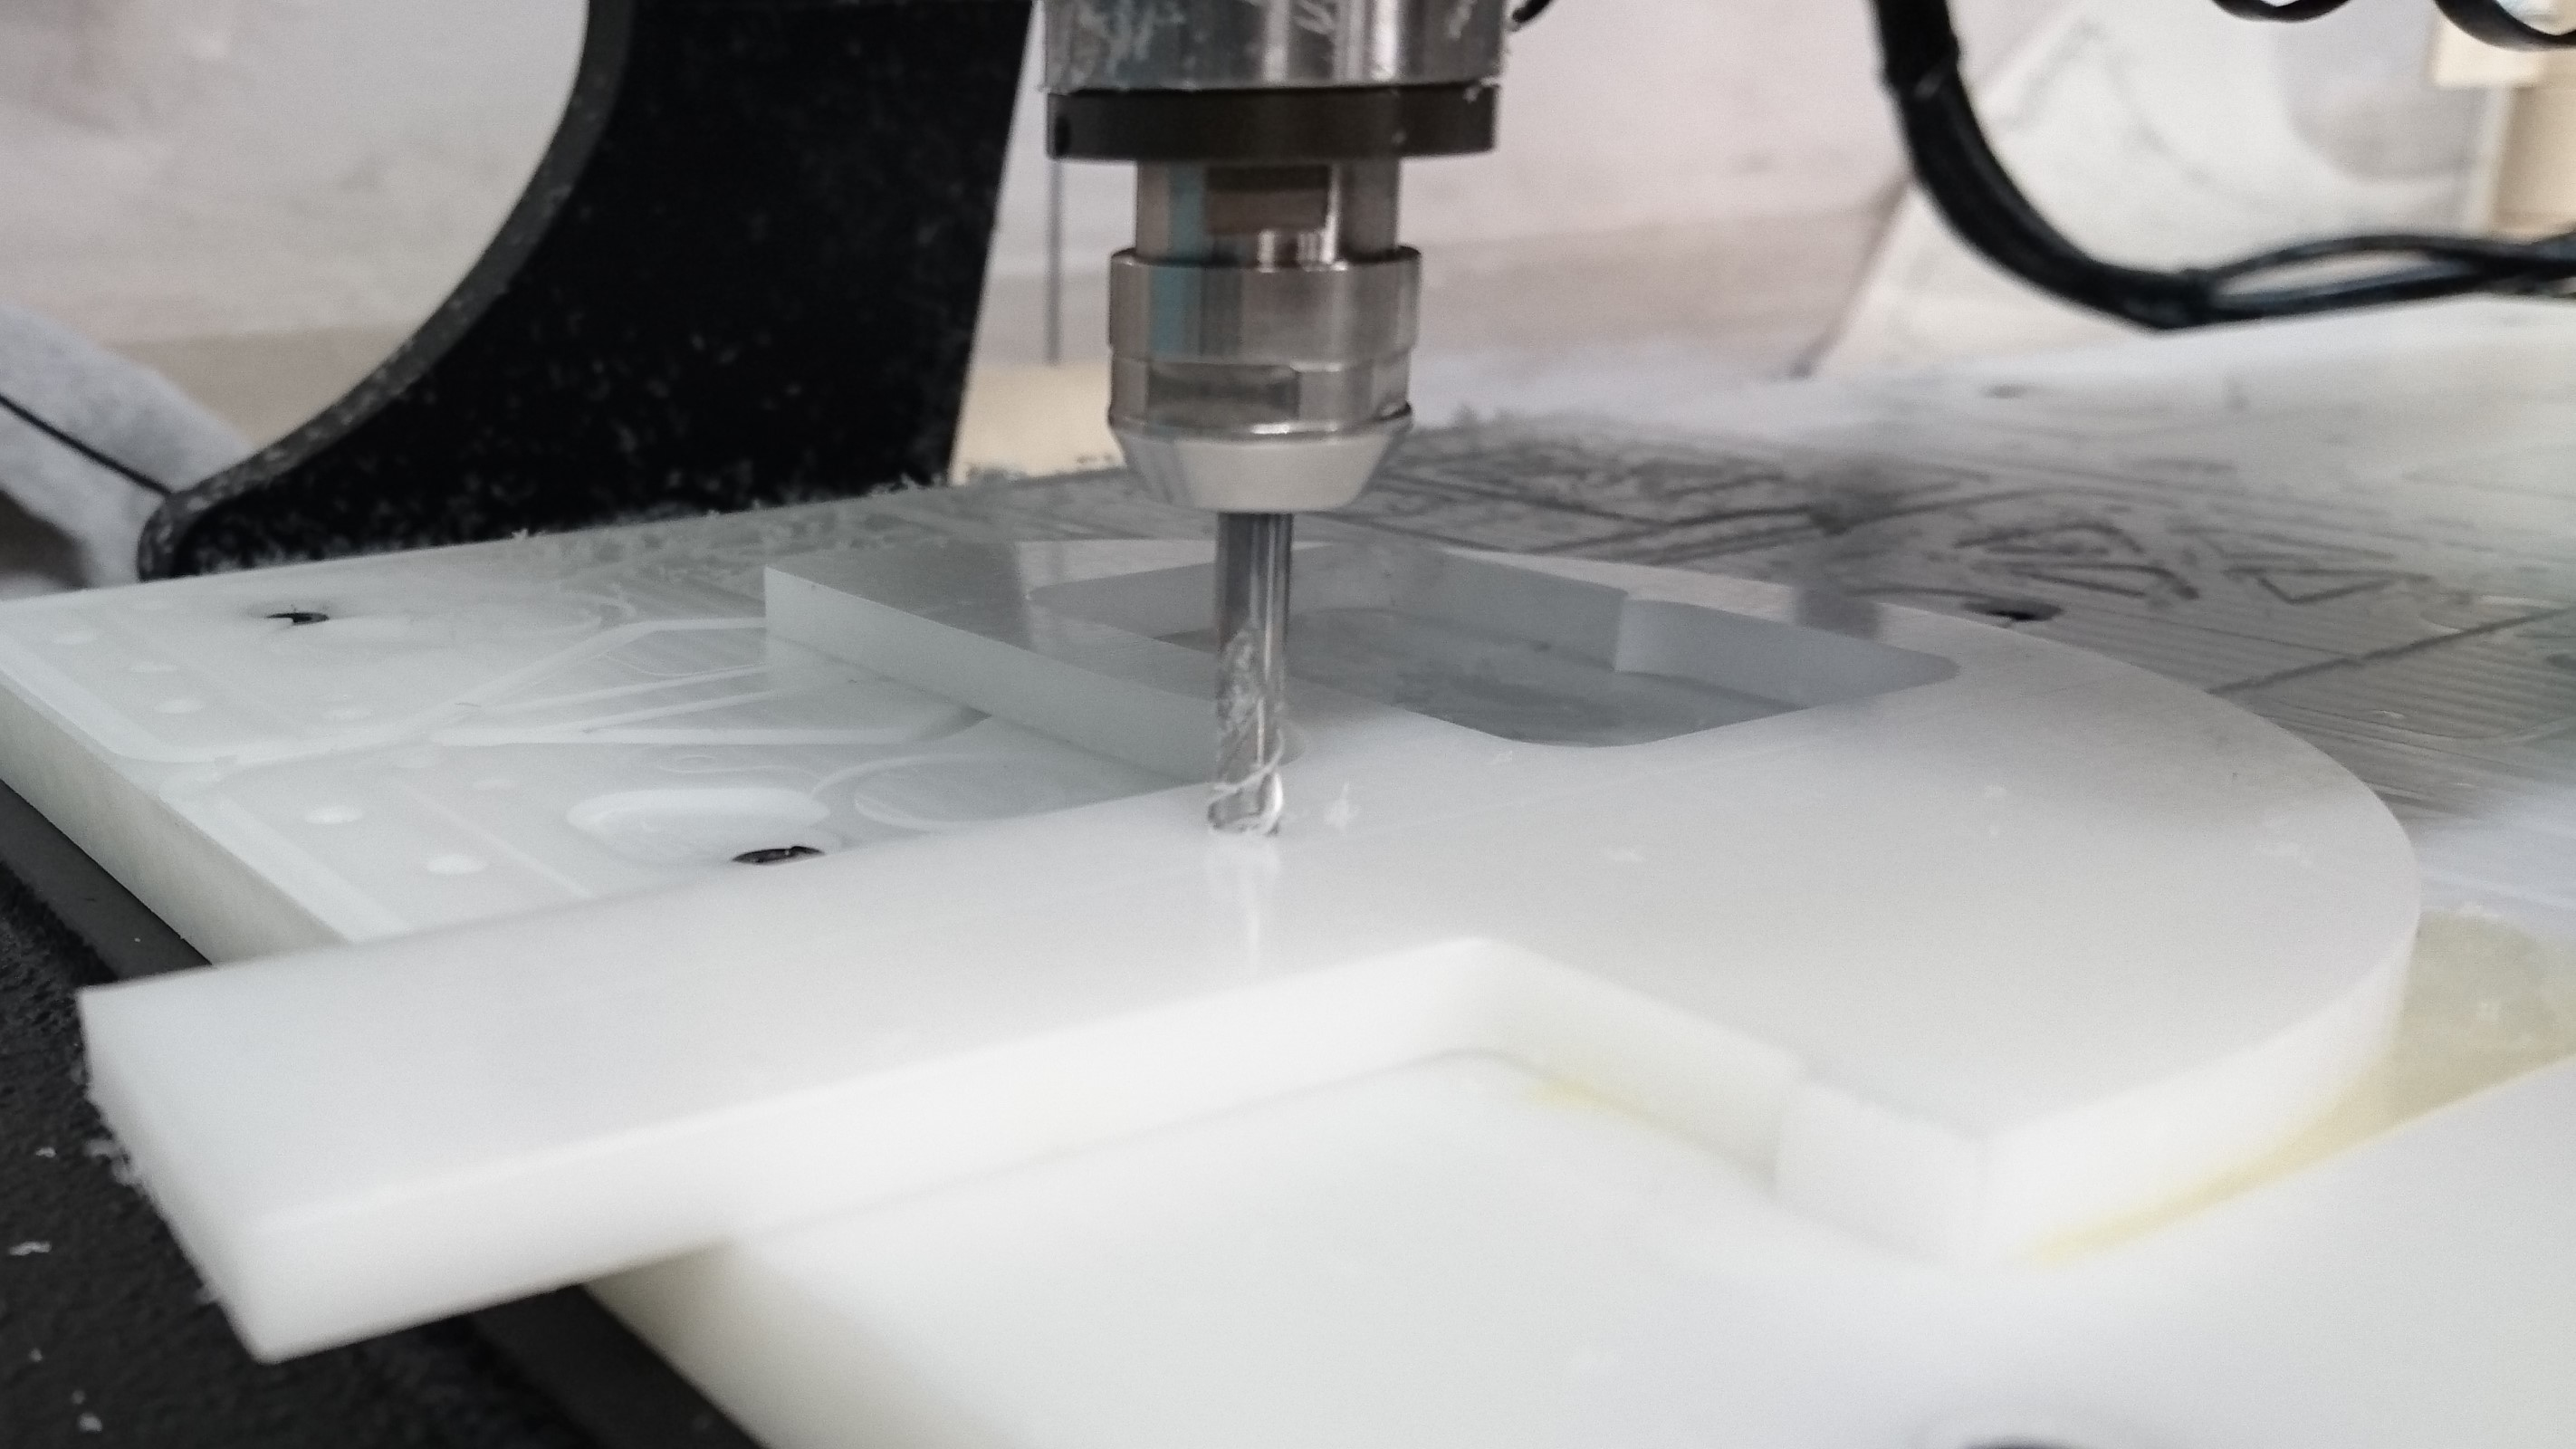
\includegraphics[width=\columnwidth]{endmill_push.jpg}
    \end{minipage}
    \caption{エンドミルの位置合わせ\label{push}}
  \end{center}
\end{figure*}

%%画像*2 エンドミルのアップ 押し付け部分のアップ endmill_4mm_side.jpg endmill_push.jpg

\clearpage
\subsection{原点合わせ}
エンドミルの固定が終わったら、まずZ軸方向の原点合わせを行います。エンドミルが自重で材料に押し付けられた位置で固定されているはずなので、その点をZ軸の原点とします。原点を合わせる際は、図\ref{zeropoint}にあるように画面右上にある原点ボタンを軸に応じてクリックしてください。 クリックした後にワーク座標タブに切り替えると、エンドミル位置がワーク座標系で0になっていることが確認できます。その後、エンドミルを少しZ軸上方向に上げた後に、XY軸方向の原点合わせを行います。USBCNCでは矢印キーでXY軸方向(水平平面方向)の移動、PgUp.DnでZ軸方向(高さ方向)の移動を行えます。エンドミルの回転軸が材料の左手前の端ギリギリになるまで動かした後に、さらに少し右奥に動かしてそこを原点とします。再度X軸とY軸について、同じように原点ボタンを押してください。材料を固定する際に回転方向に少しずれてしまうと、加工領域の長方形が材料からはみ出てしまうため、図\ref{milling_image}のように材料の端ではなく少し内側を原点とすることで、加工領域のマージンを取っています。全ての軸について原点を合わせ終わったら再度resetボタンを押して、加工目安時間が再度表示されたら加工が可能になります。\\
\begin{figure*}[tbh]
  \begin{center}
    \begin{minipage}{0.6\columnwidth}
      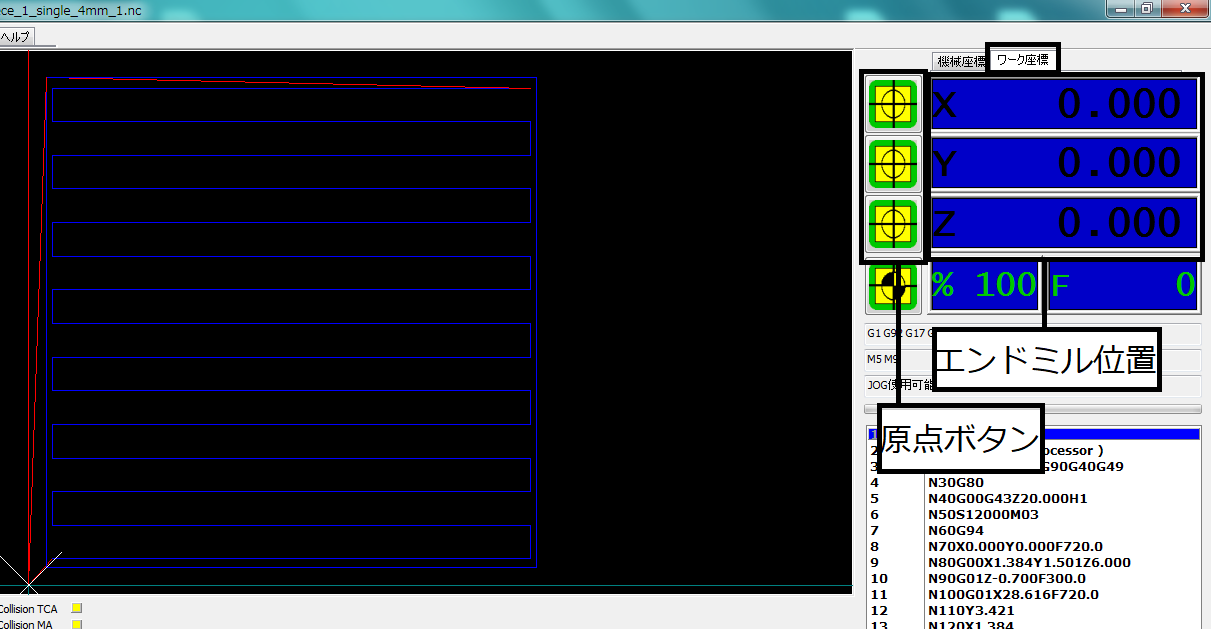
\includegraphics[width=\columnwidth]{zeropoint_trim.png}
    \end{minipage}
    \caption{原点合わせ(USBCNC)\label{zeropoint}}
    \begin{minipage}{0.6\columnwidth}
      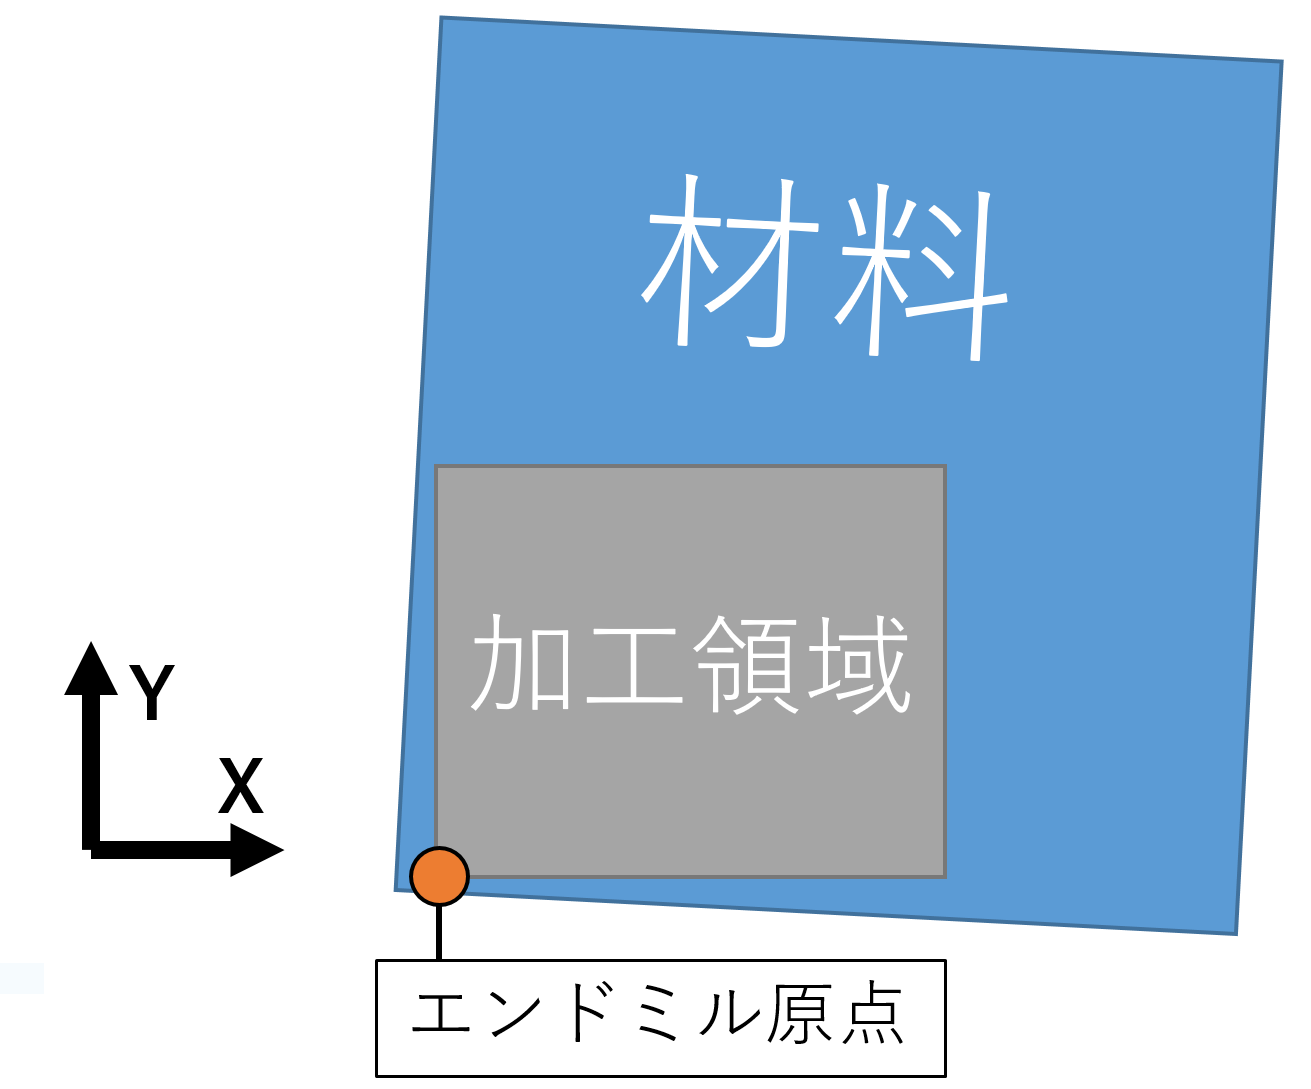
\includegraphics[width=\columnwidth]{milling_image.png}
    \end{minipage}
    \caption{XY軸の原点合わせ\label{milling_image}}
  \end{center}
\end{figure*}

%%画像*2 原点設定方法 位置合わせの説明 zeropoint_trim.png milling_image.png

\clearpage
\subsection{加工}
セッティングが終わったら、加工を開始します。CNCでの加工は材料が剥がれる・エンドミルが折れるなどの事故が起きることがあるので、その際には緊急停止できるように気をつけましょう。USBCNCの場合は、F6ボタンが加工一時停止ボタンになっています。CNCの剛性にもよりますが、樹脂を削る際はドライ(切削油を使わないこと)で、金属を削る際は切削油を使って加工することが多いようです。加工中の様子を見つつ、工具のパラメータや速度などを調整してください。一通り加工が終わったら、材料を剥がす前に削り残しが無いかのチェックを行います。削り残しがあった場合は、再度Z軸の原点合わせをした後に、外形だけ削り直すなどの方法で対応できます。少しの削り残しであればバリ取りカッターなどで取り除けるので、様子を見ながら削り直すかどうかを決めてください。加工については、経験的で身に付く部分も多いので、失敗を繰り替えして学ぶ必要があります。\\

\begin{figure*}[tbh]
  \begin{center}
    \begin{minipage}{0.7\columnwidth}
      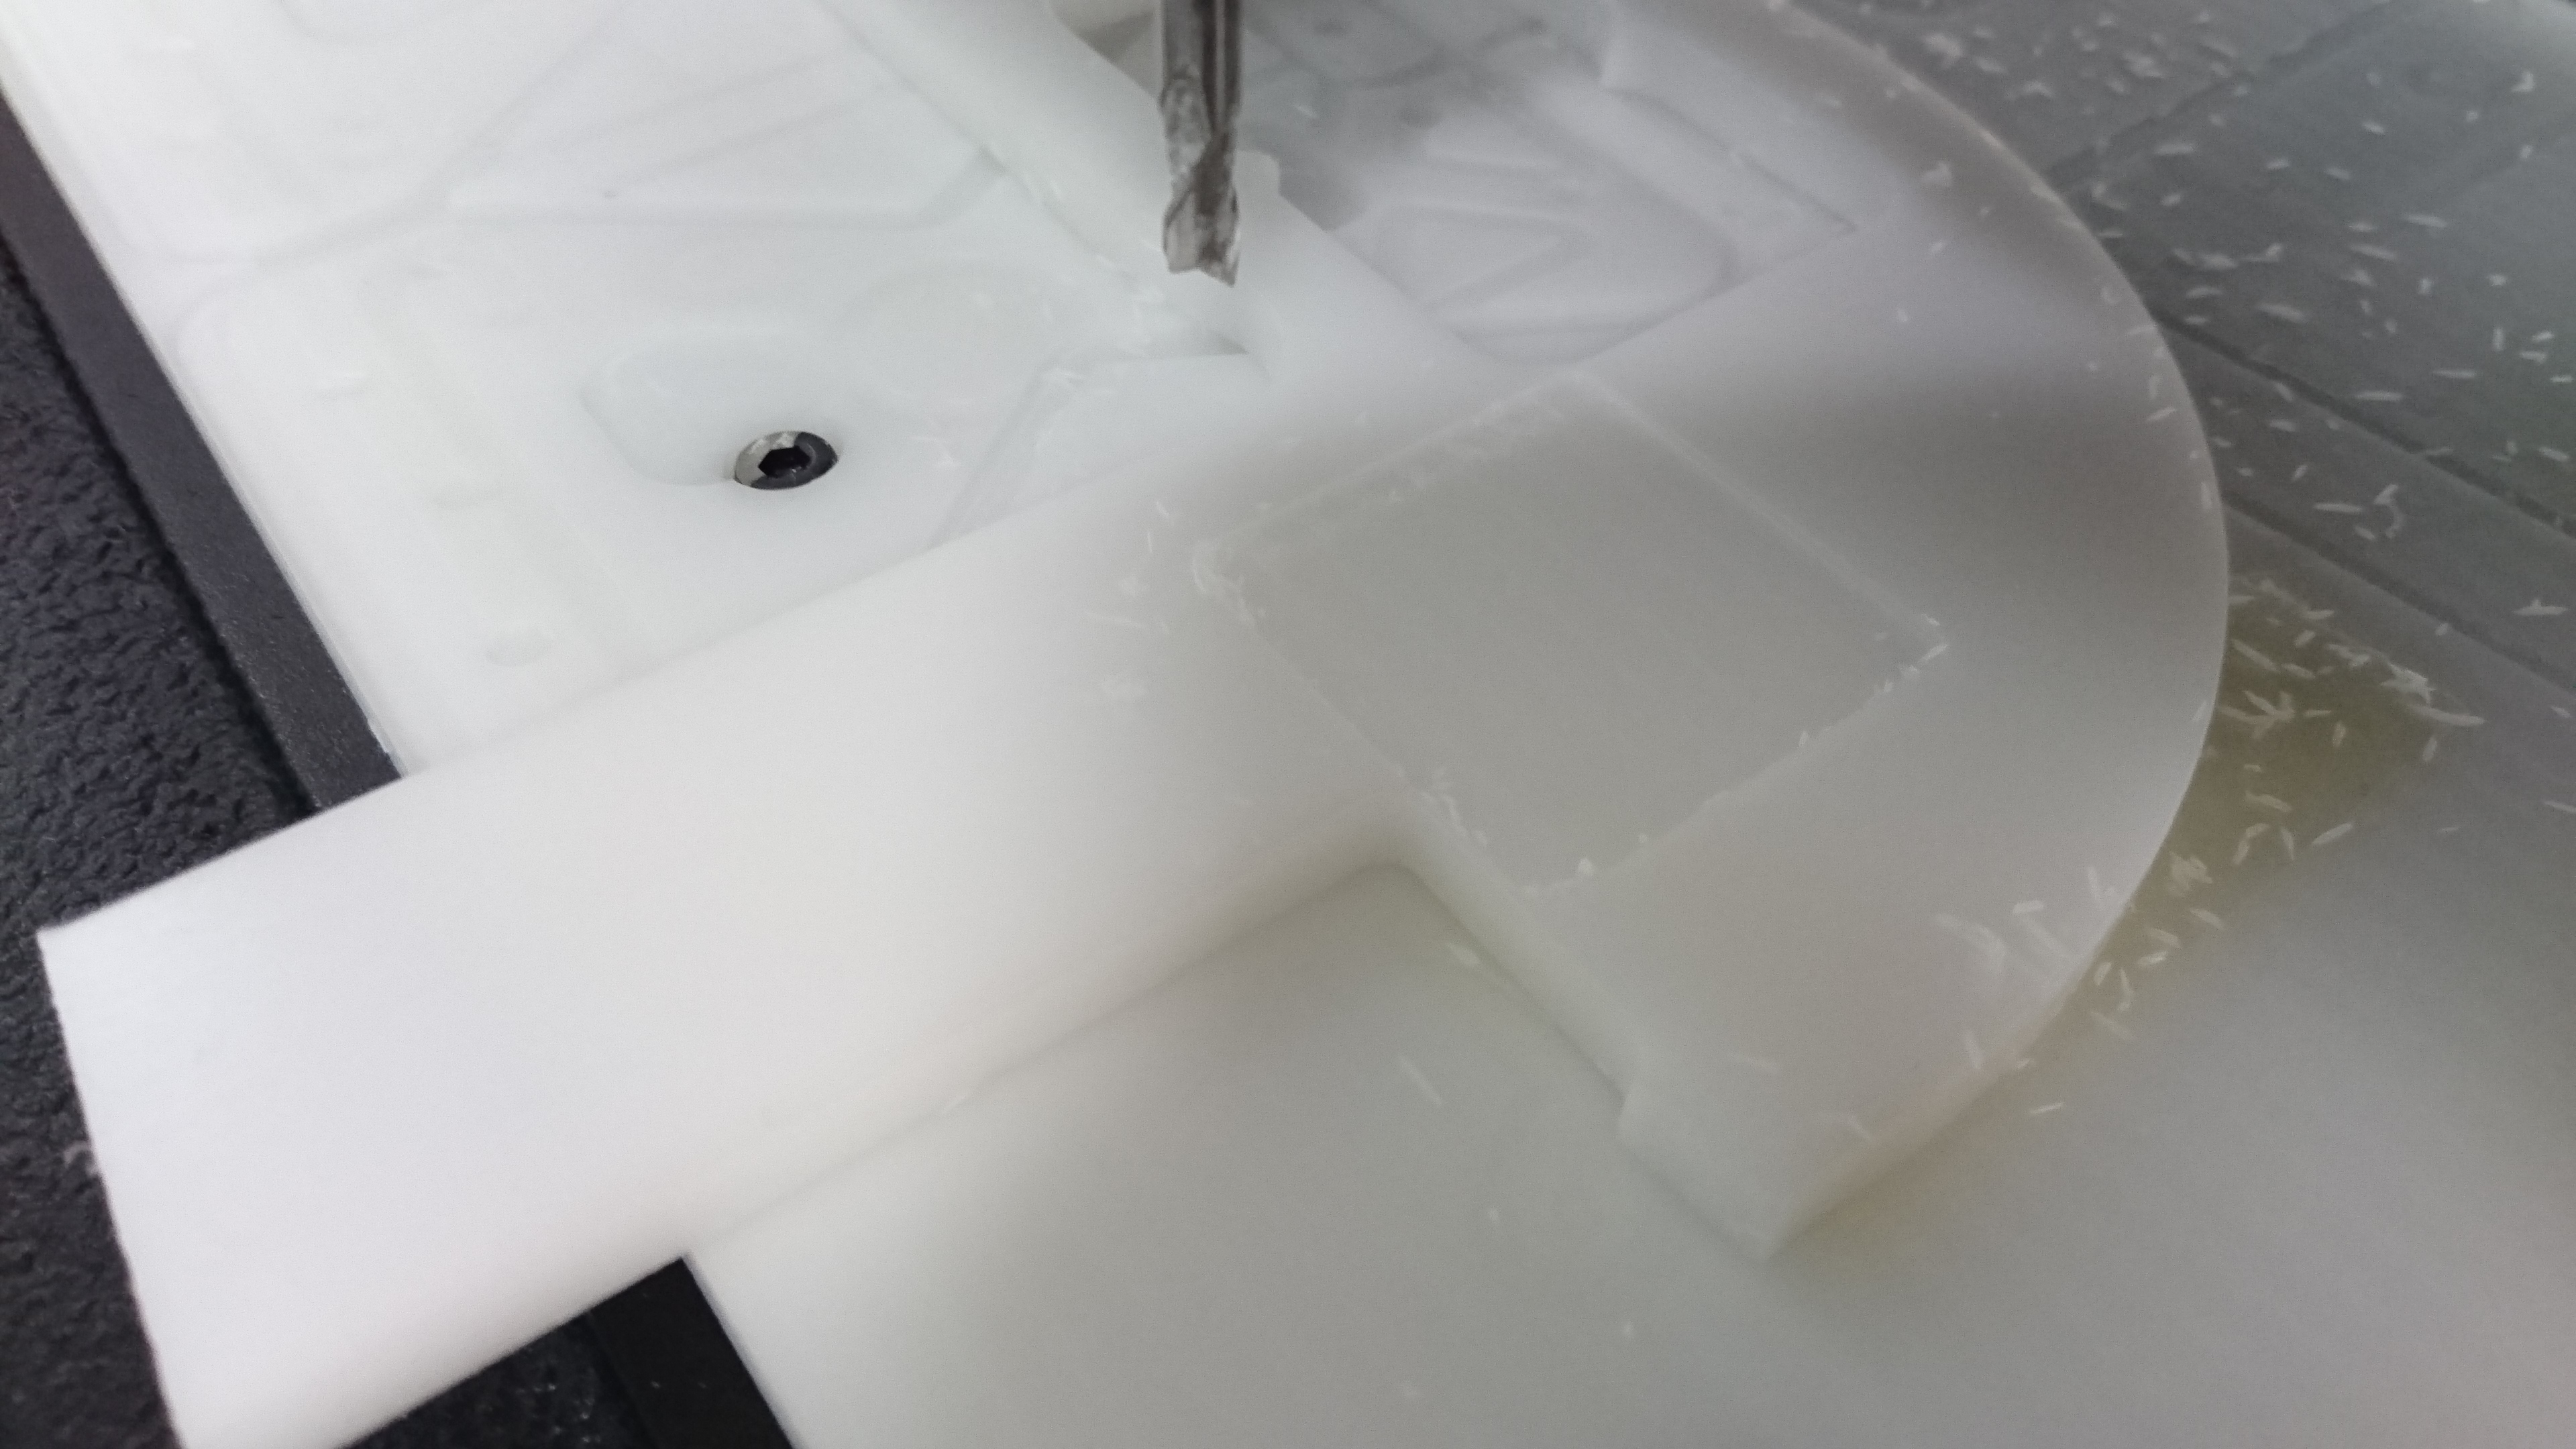
\includegraphics[width=\columnwidth]{pocket_milling_now.jpg}
    \end{minipage}
    \caption{ポケット加工\label{pocket_now}}
    \begin{minipage}{0.7\columnwidth}
      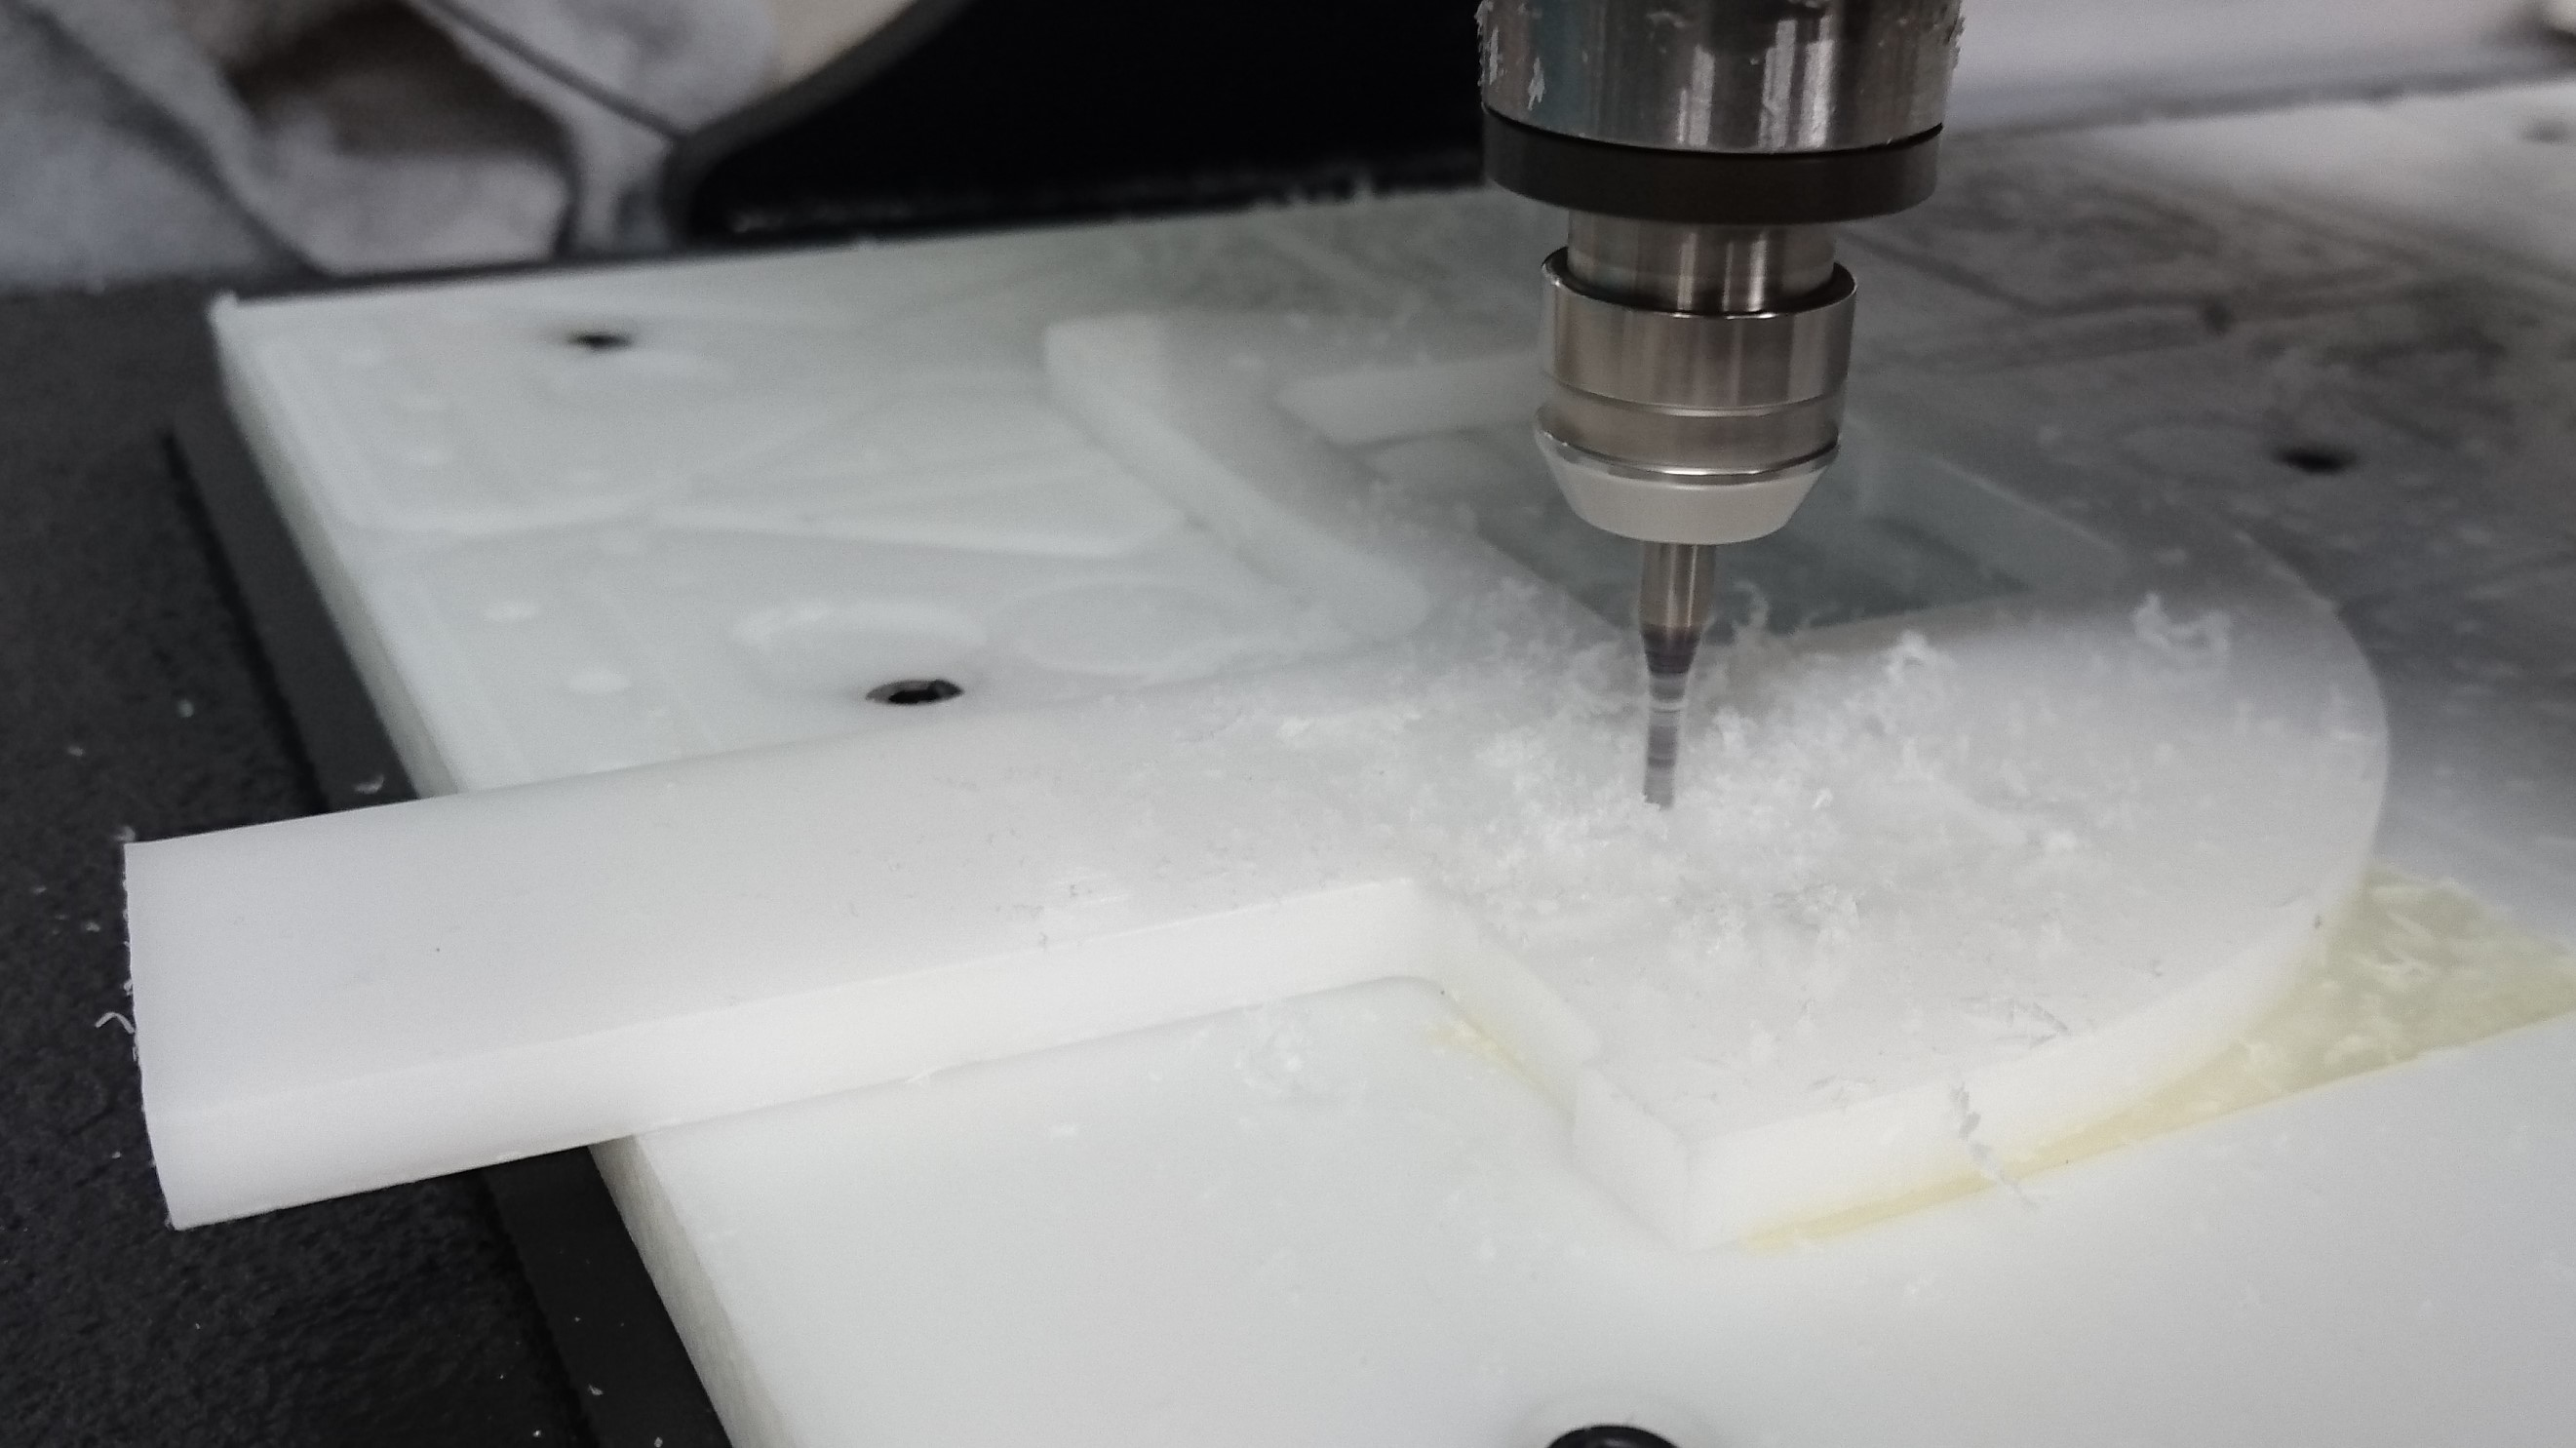
\includegraphics[width=\columnwidth]{milling_now_trim.jpg}
    \end{minipage}
    \caption{外周の切り抜き加工\label{outer_now}}
  \end{center}
\end{figure*}

%%画像*2 ポケット加工中の画像 輪郭加工中の画像 pocket_milling_now.jpg milling_now_trim.jpg

\clearpage
今回の加工では、最初のポケット加工に4mmのエンドミル、その後の加工に2mmのエンドミルを用いているため、加工ファイルが2つに分かれていて、途中でエンドミルの交換を行う必要があります。この場合、基準平面を一定にするために、交換後にZ軸方向の原点合わせを再度行う必要があります。この時気を付けるのが、XY方向の原点位置を変えないことです。エンドミルを交換して、図\ref{zeropoint_again}のように基準平面位置にエンドミルを押し付けたら、Z軸のみ原点ボタンを押します。この時に間違えてXY軸の原点ボタンも押しがちなので、気を付けてください。もし押してしまった場合、前の加工ファイルと次の加工ファイルの原点位置が異なってしまうため、正しく加工を行うことができなくなります。\\

\begin{figure*}[tbh]
  \begin{center}
    \begin{minipage}{0.6\columnwidth}
      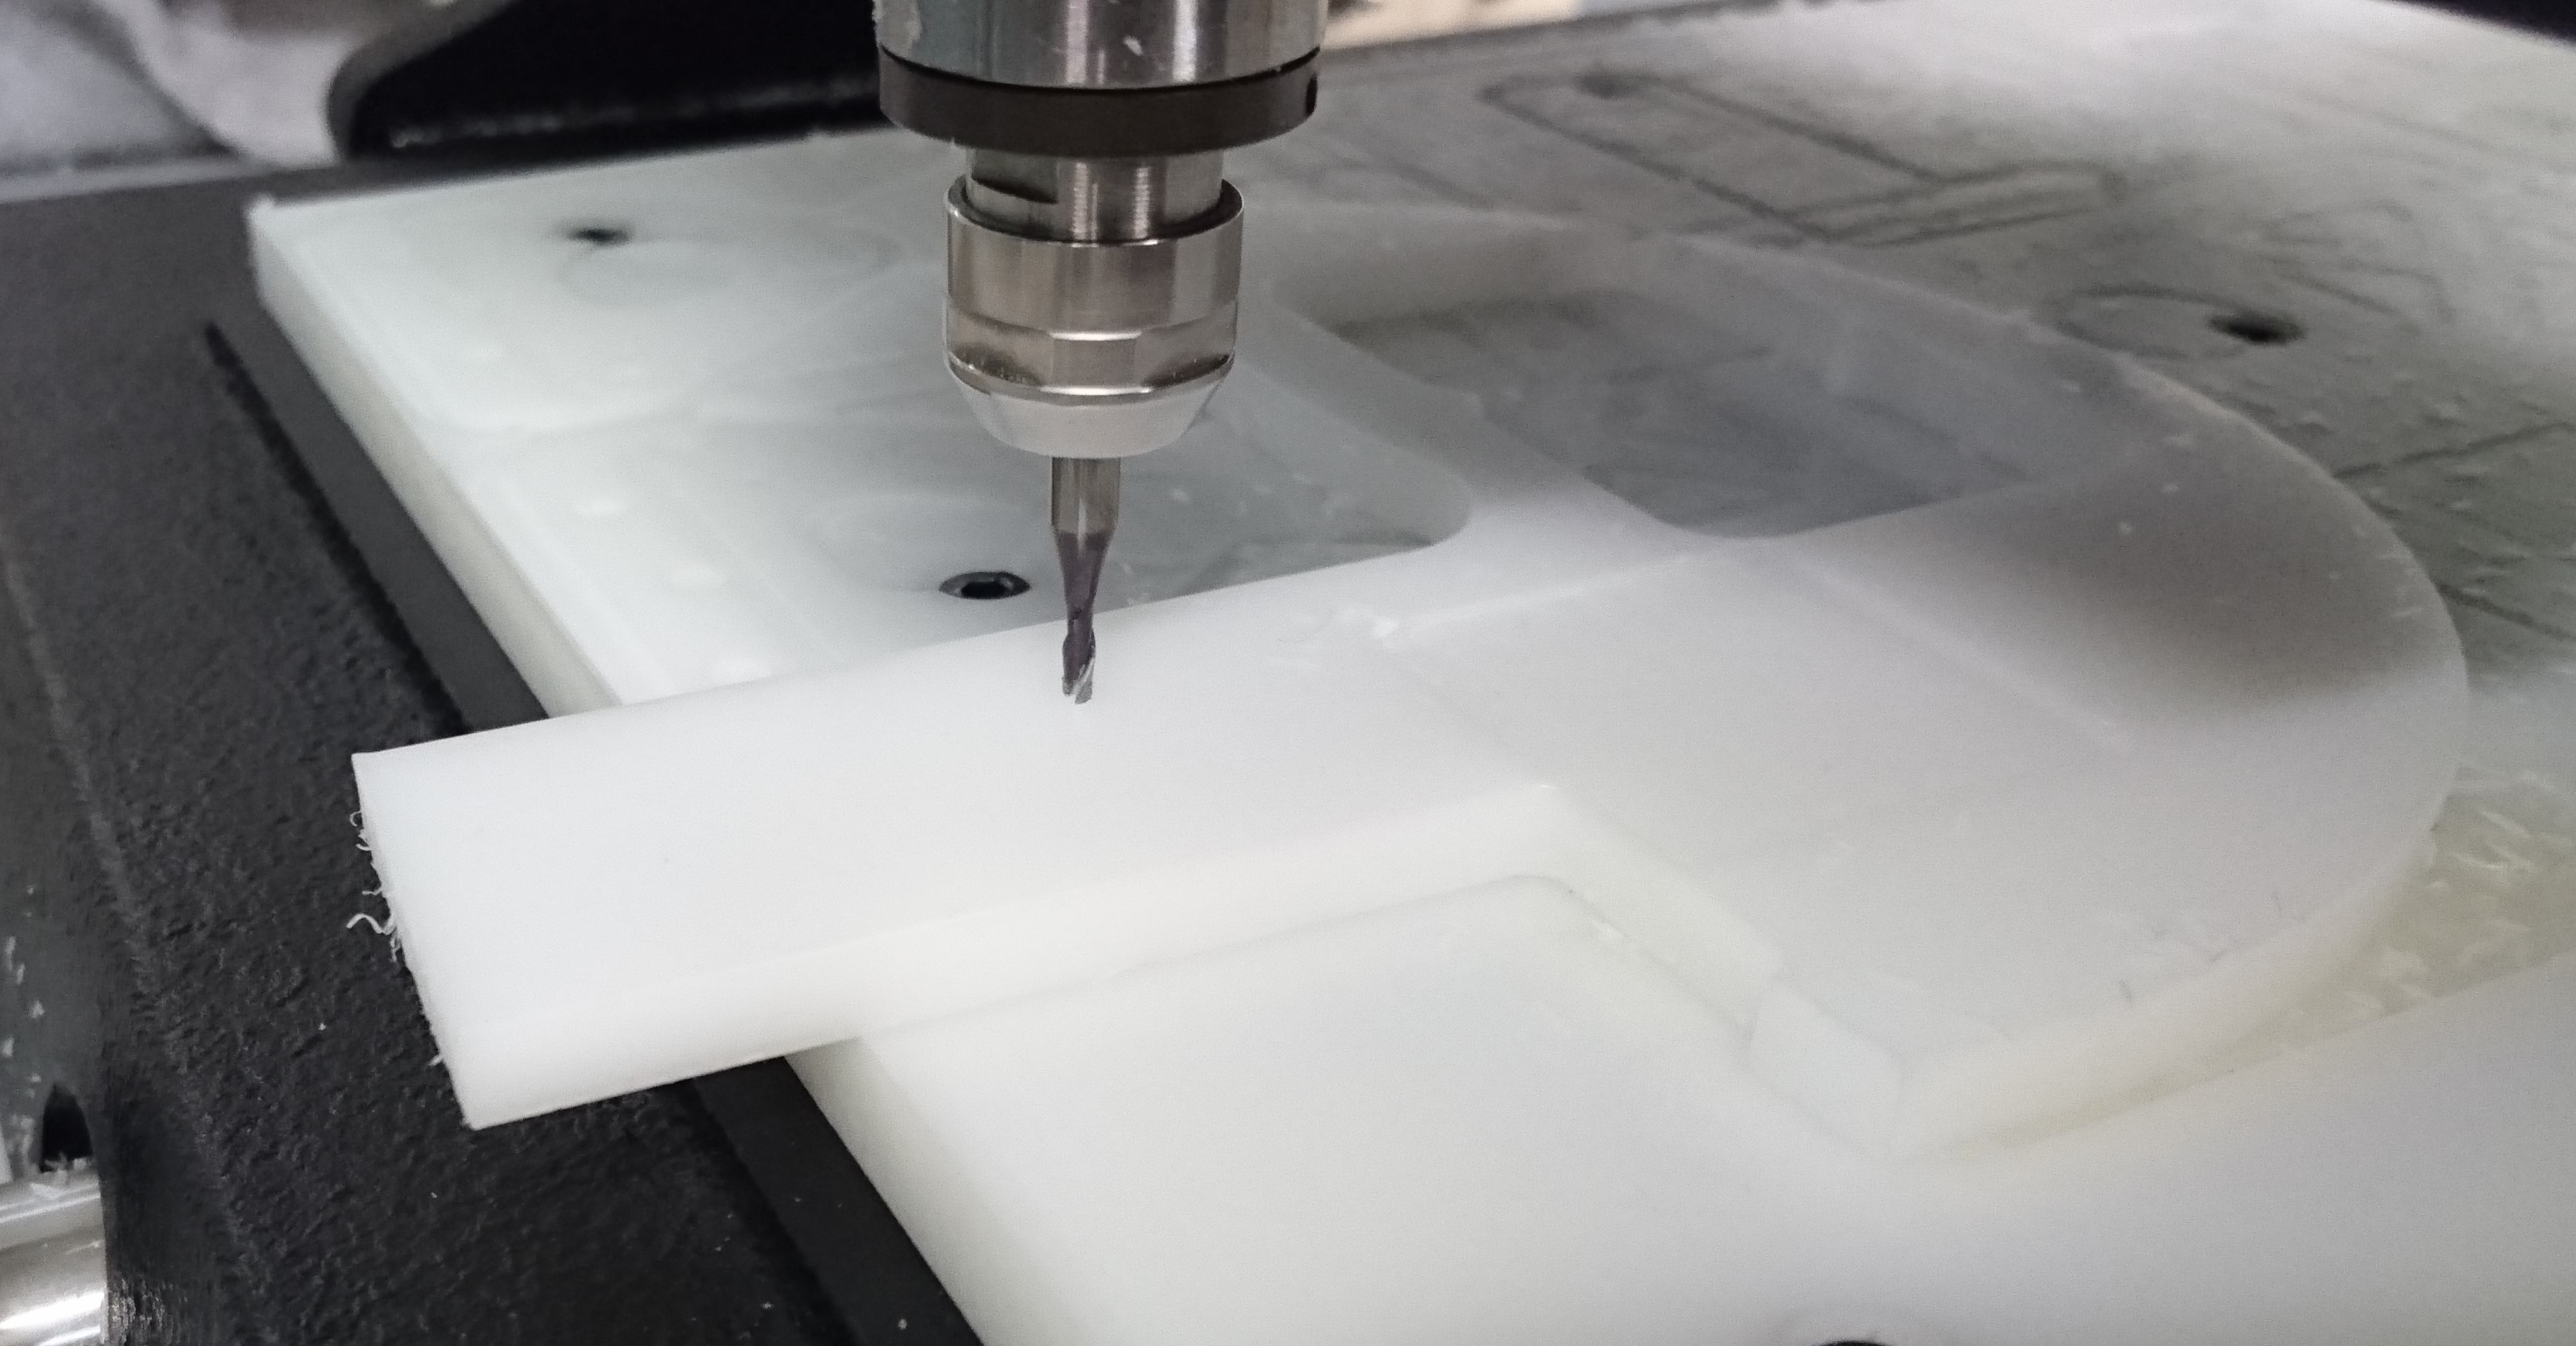
\includegraphics[width=\columnwidth]{zeropoint_again.jpg}
    \end{minipage}
    \caption{原点の再設定\label{zeropoint_again}}
  \end{center}
\end{figure*}

%%画像*1 原点の再設定の画像 zeropoint_again.jpg

\subsection{清掃}
加工が終わったら、まず切り子を清掃します。掃除機で吸い取ったり、卓上サイズの箒・ちりとりなどで清掃を行って下さい。その後、材料を捨て板から剥がします。図\ref{after_milling}の用に材料が捨て板に張り付いて手で取りにくい場合には、ヘラやノミを捨て板と材料の間に差し込んで剥がします。材料を剥がした後に、捨て板に残った両面テープをすべて剥がして綺麗にします。パーツクリーナーなどを使うと接着剤が溶けてベタベタになるので、なるべくヘラや手で剥がすのをおすすめします。加工時の熱で両面テープと捨て板と間の粘着が強くなって、剥がすのが困難になる場合もあるので、その場合はパーツクリーナーも使いつつ根気よく清掃を行って下さい。捨て板が綺麗になったら清掃の終了です。\\

\begin{figure*}[tbh]
  \begin{center}
    \begin{minipage}{0.5\columnwidth}
      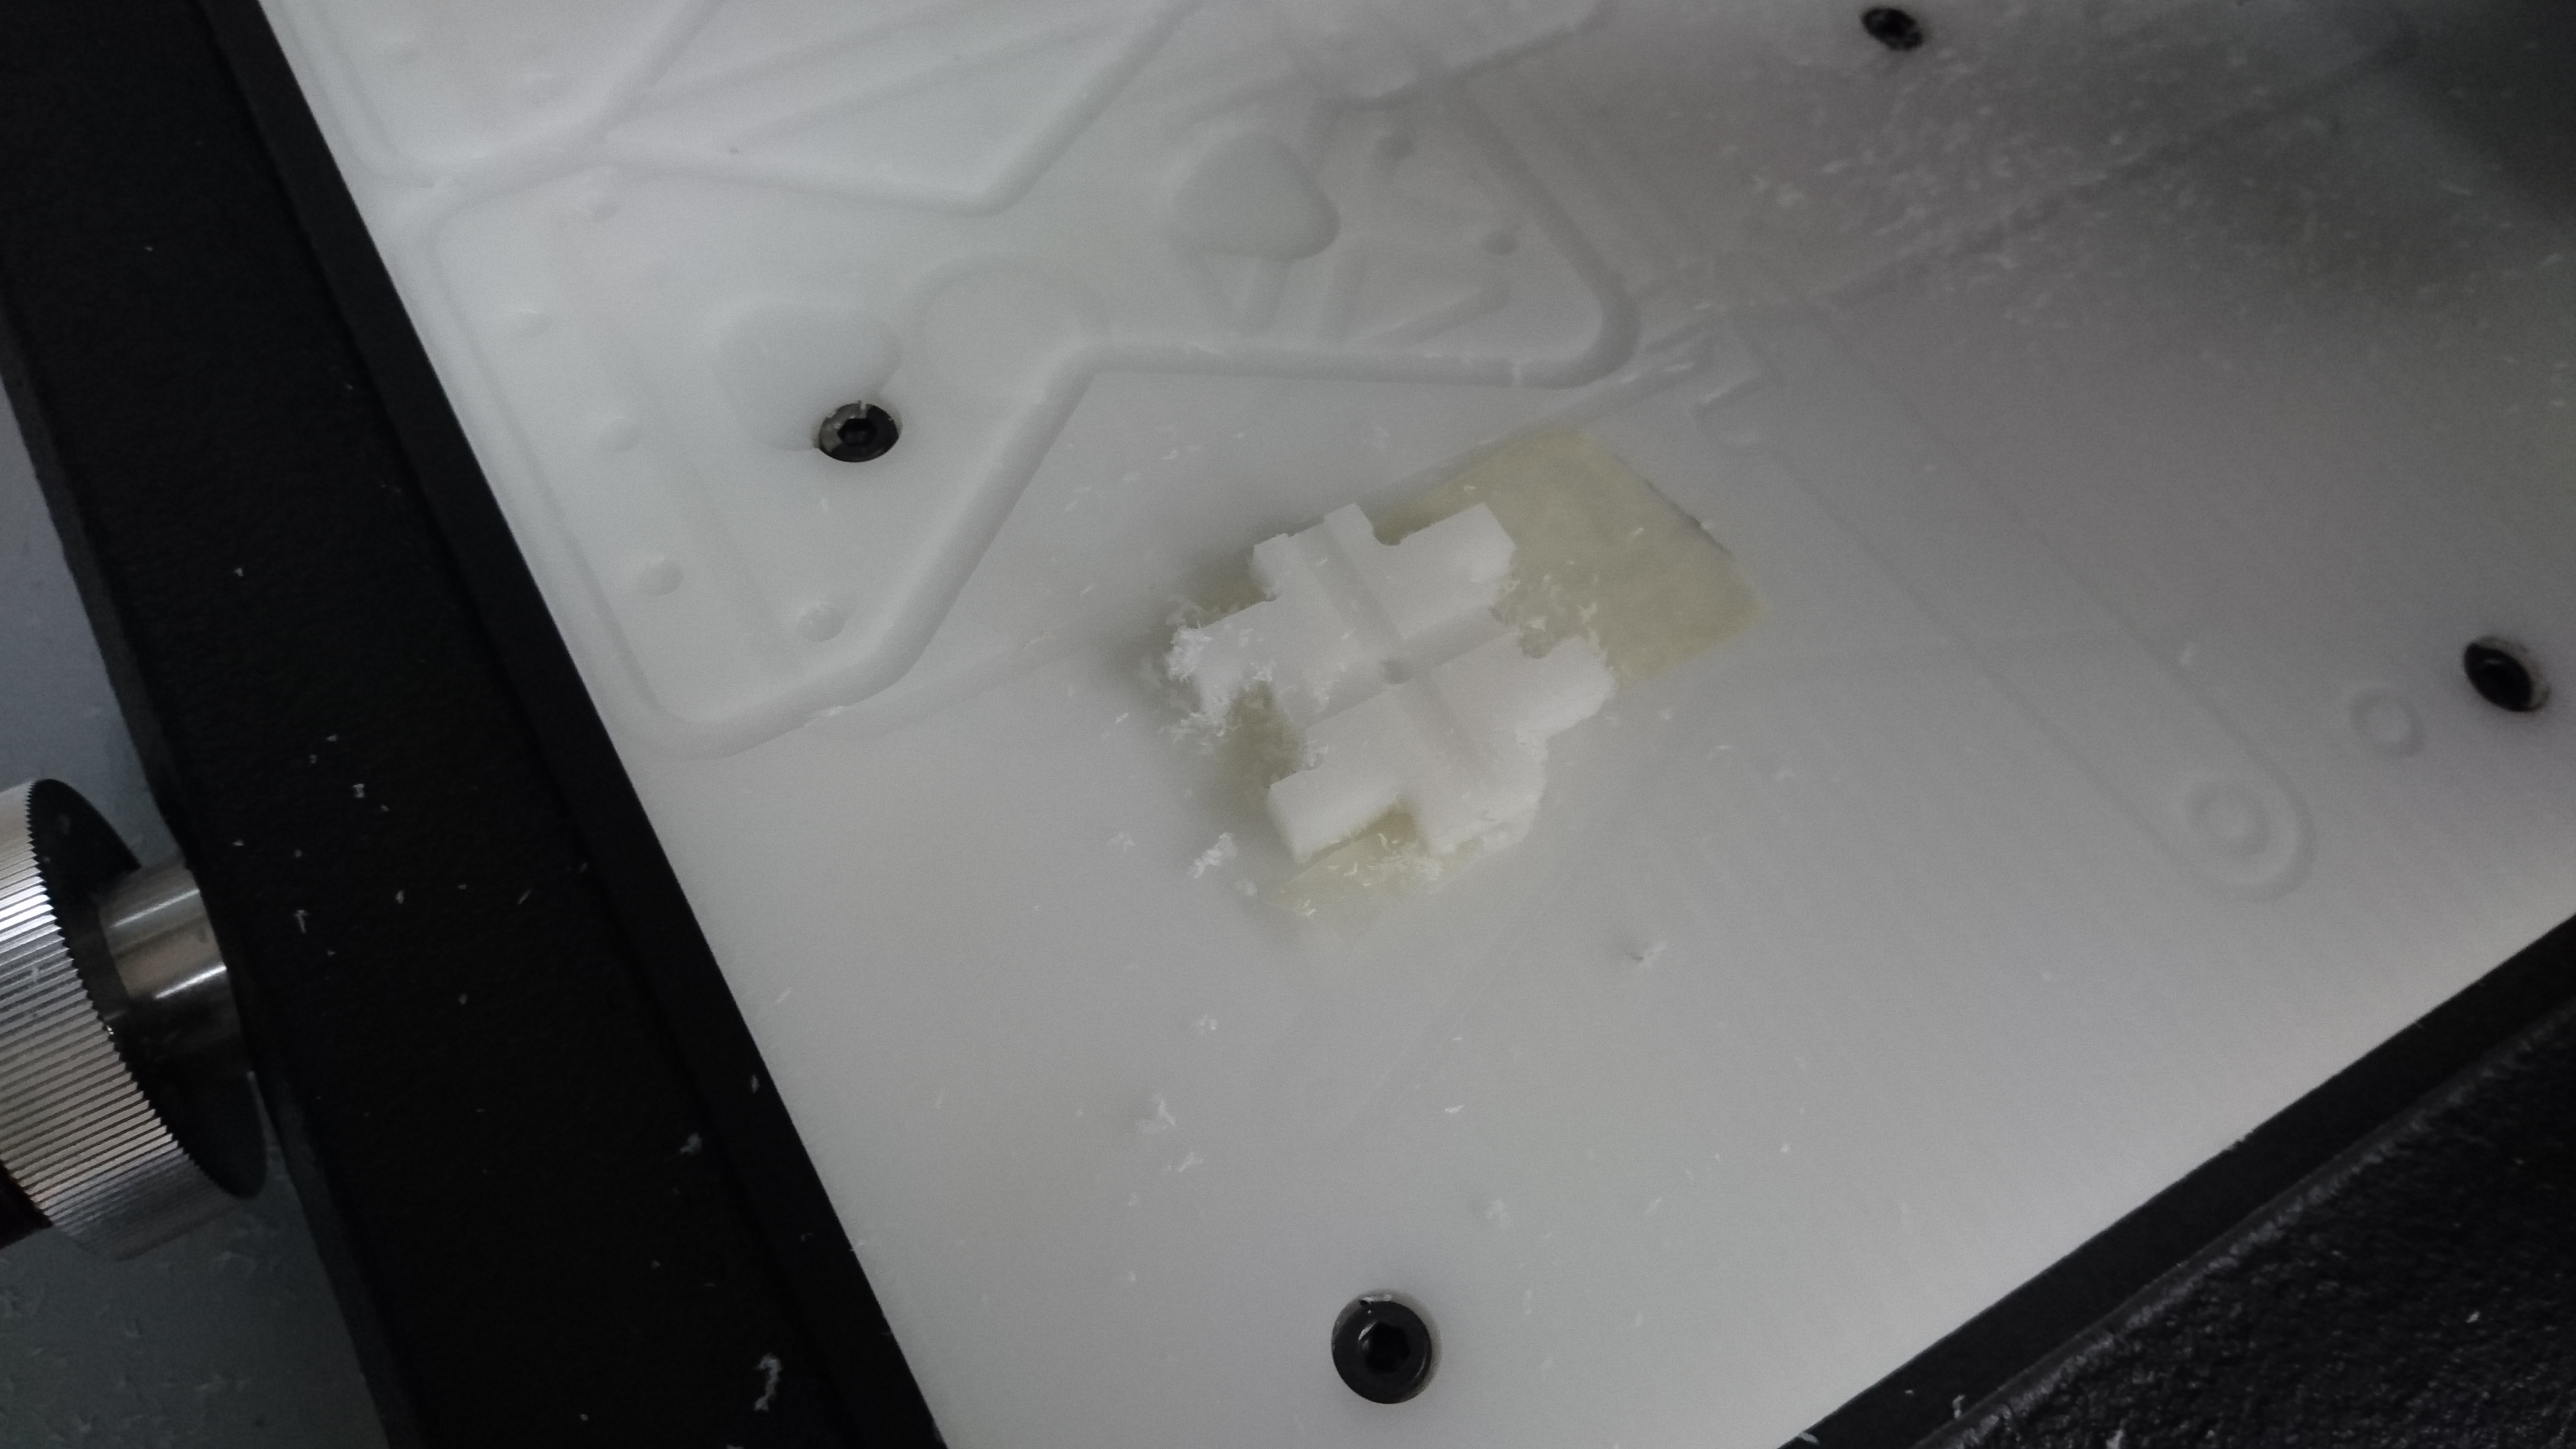
\includegraphics[width=\columnwidth]{after_milling.jpg}
    \end{minipage}
    \caption{加工後の様子\label{after_milling}}
  \end{center}
\end{figure*}

%%画像*1 剥がした後の画像 after_milling.jpg

\clearpage
\subsection{仕上げ}
最後に、パーツの仕上げを行います。エンドミルの状態や削り残しの有無にもよりますが、図\ref{parts_bari}のようにバリが残っている場合に仕上げが必要になります。CNC加工部品の仕上げにはバリ取りカッター(図\ref{baritori})やドリルが便利です。バリ取りカッターは外周に残ったバリの除去、ドリルは穴の部分の削り残しや溶けて穴から盛り上がった樹脂の除去に使います。自分の満足の行くまで仕上げができたら、部品の完成です。完成したものが図\ref{parts_nobari}になります。図\ref{thickness}のようにノギスで測ると、厚み精度も出ていることがわかります。\\

\begin{figure*}[tbh]
  \begin{center}
    \begin{minipage}{0.6\columnwidth}
      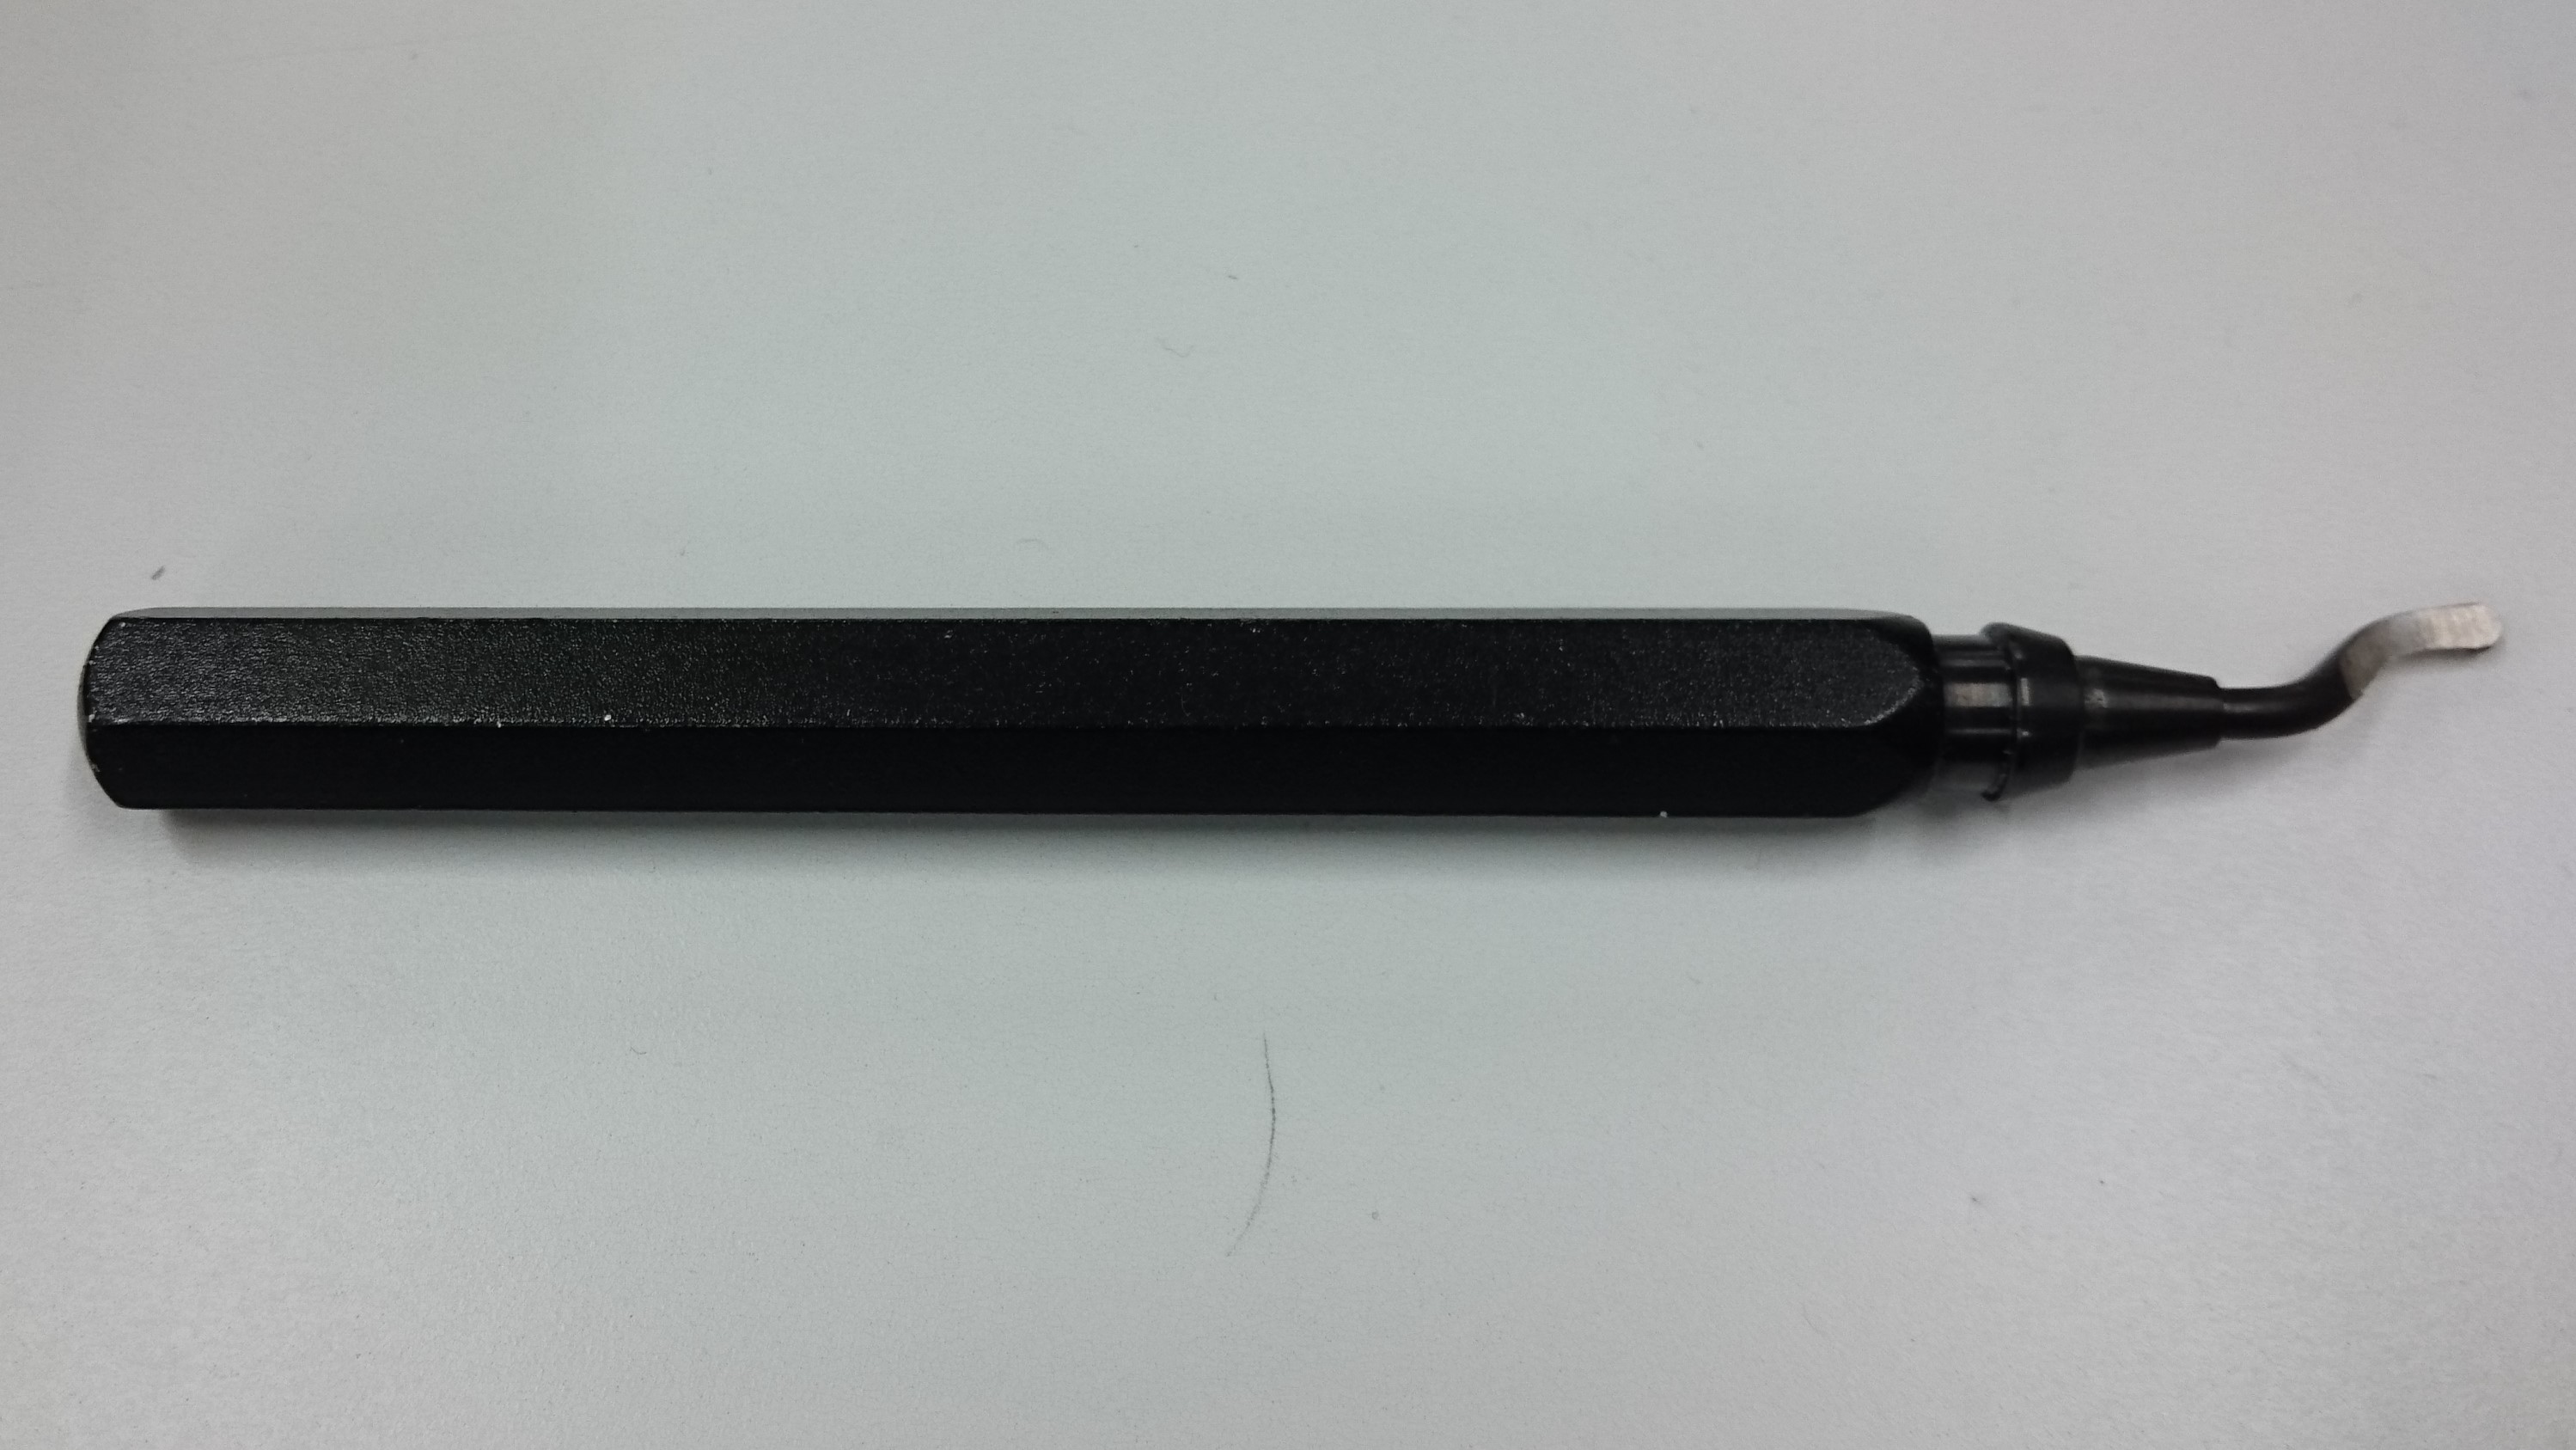
\includegraphics[width=\columnwidth]{baritori.jpg}
    \end{minipage}
    \caption{バリ取りカッター\label{baritori}}
  \end{center}
  \begin{center}
    \begin{minipage}{0.6\columnwidth}
      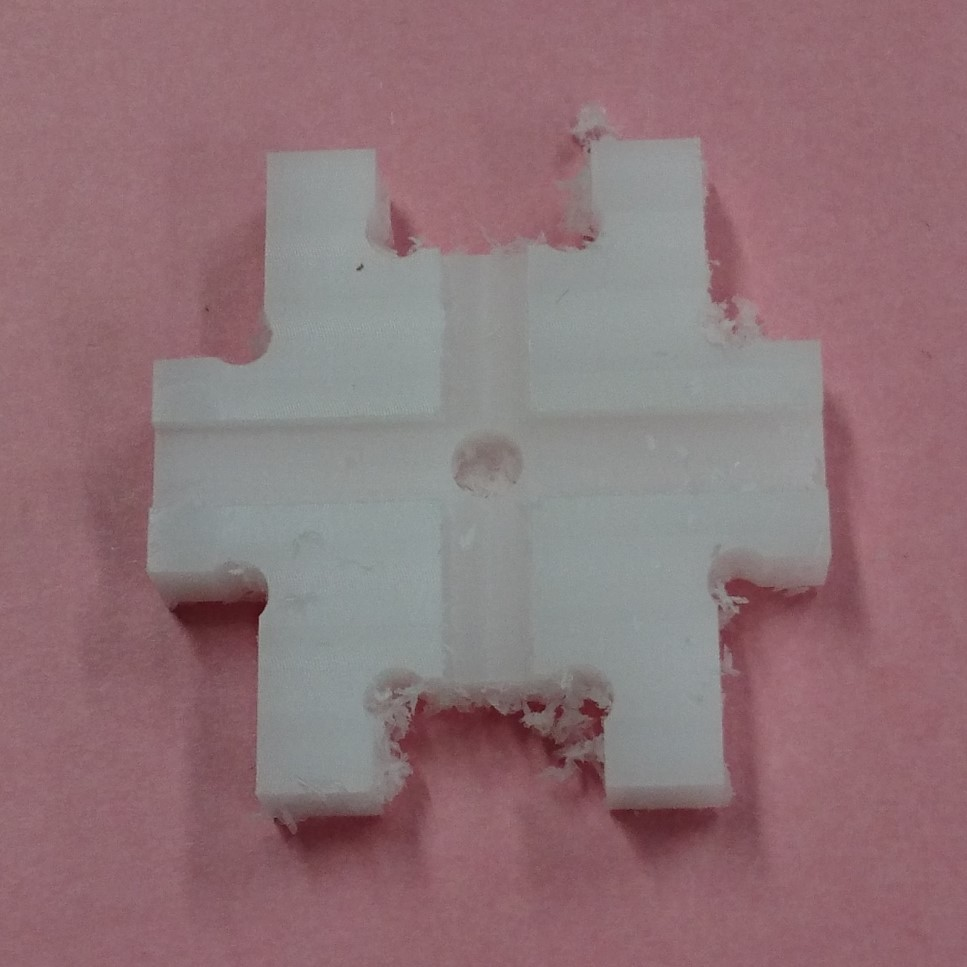
\includegraphics[width=\columnwidth]{parts_bari.jpg}
    \end{minipage}
    \caption{仕上げ前\label{parts_bari}}
  \end{center}
\end{figure*}

\begin{figure*}[tbh]
  \begin{center}
    %% \begin{minipage}{0.6\columnwidth}
    %%   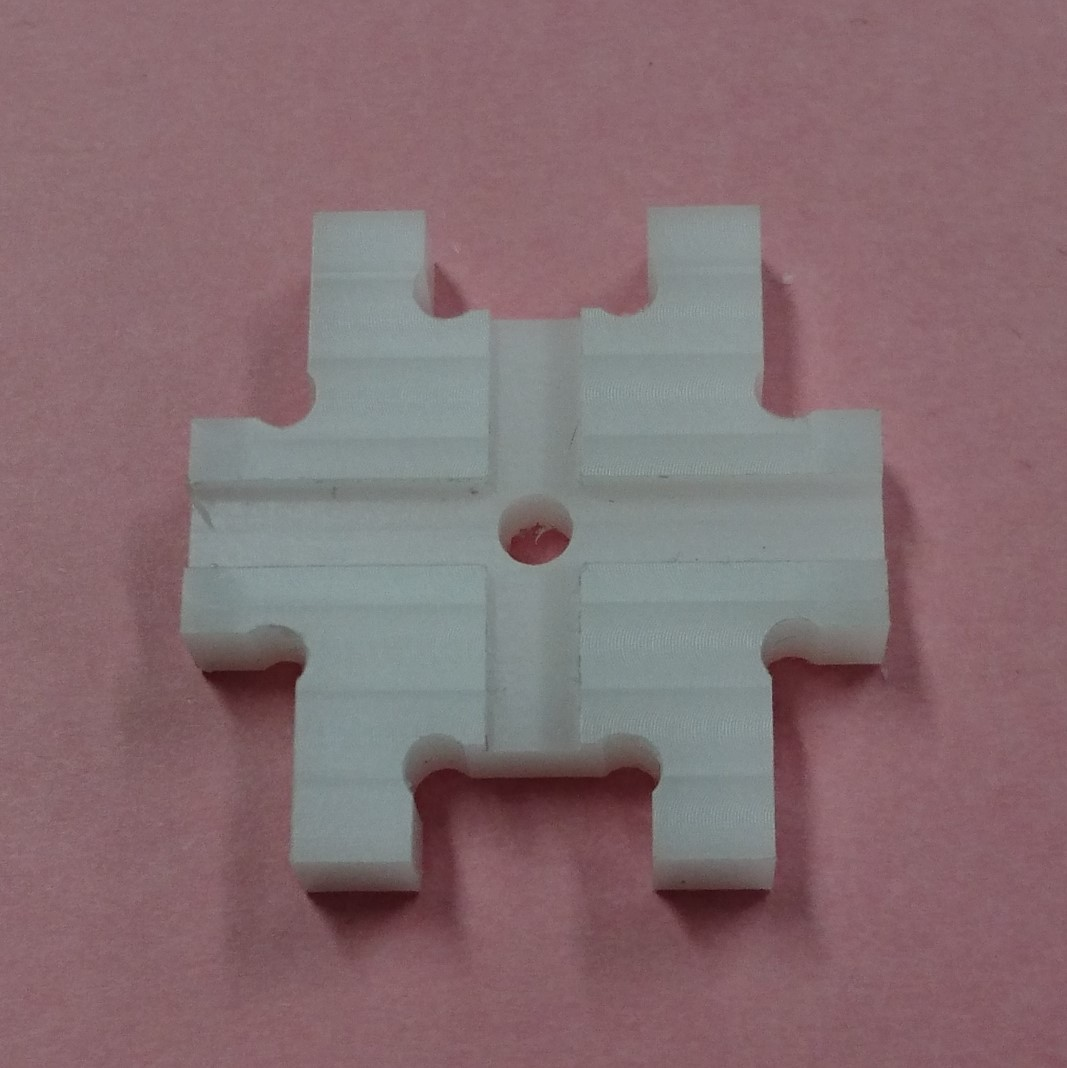
\includegraphics[width=\columnwidth]{parts.jpg}
    %% \end{minipage}
    %% \caption{仕上げ後1\label{parts_nobari1}}
    \begin{minipage}{0.7\columnwidth}
      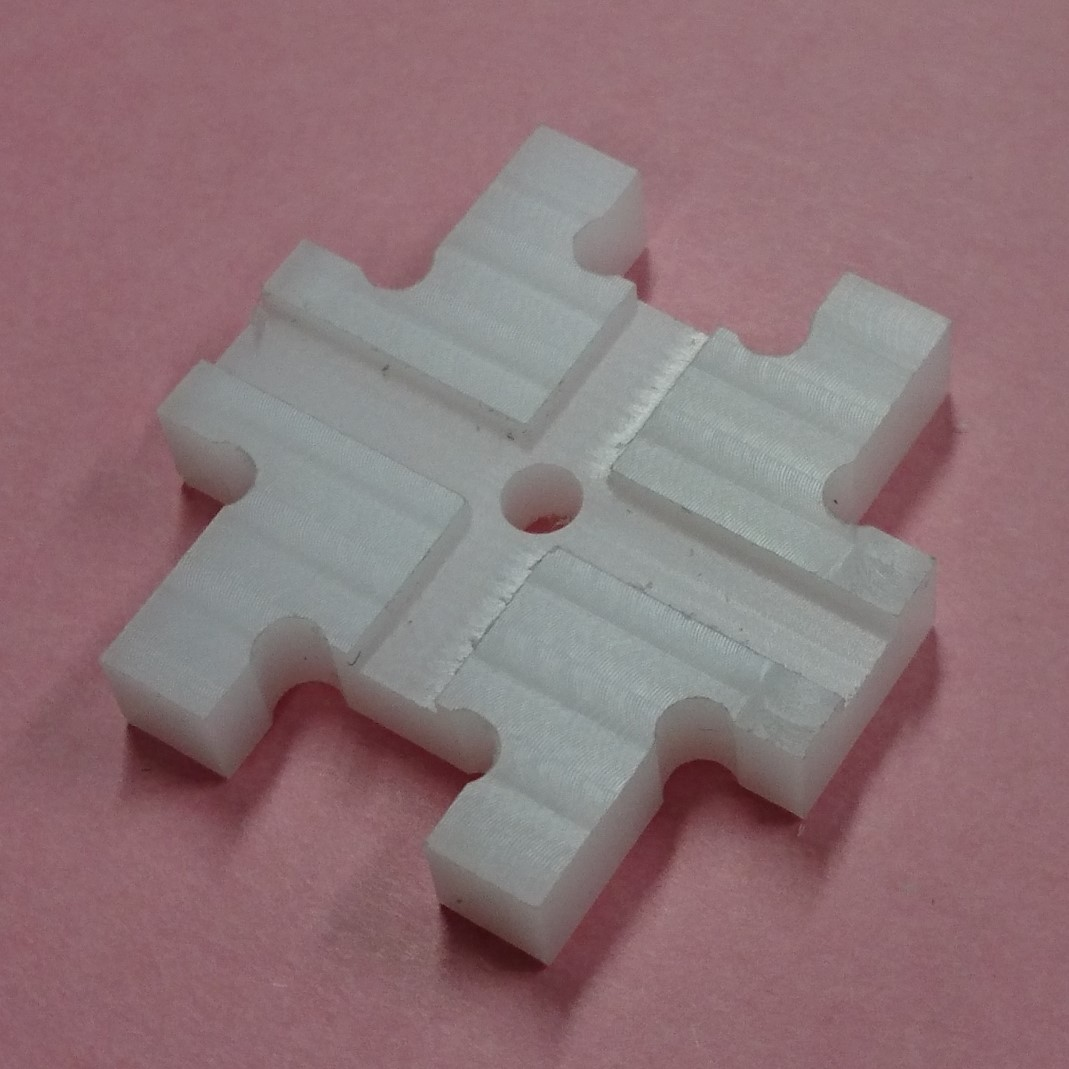
\includegraphics[width=\columnwidth]{parts_isome.jpg}
    \end{minipage}
    \caption{仕上げ後\label{parts_nobari}}
    \begin{minipage}{0.7\columnwidth}
      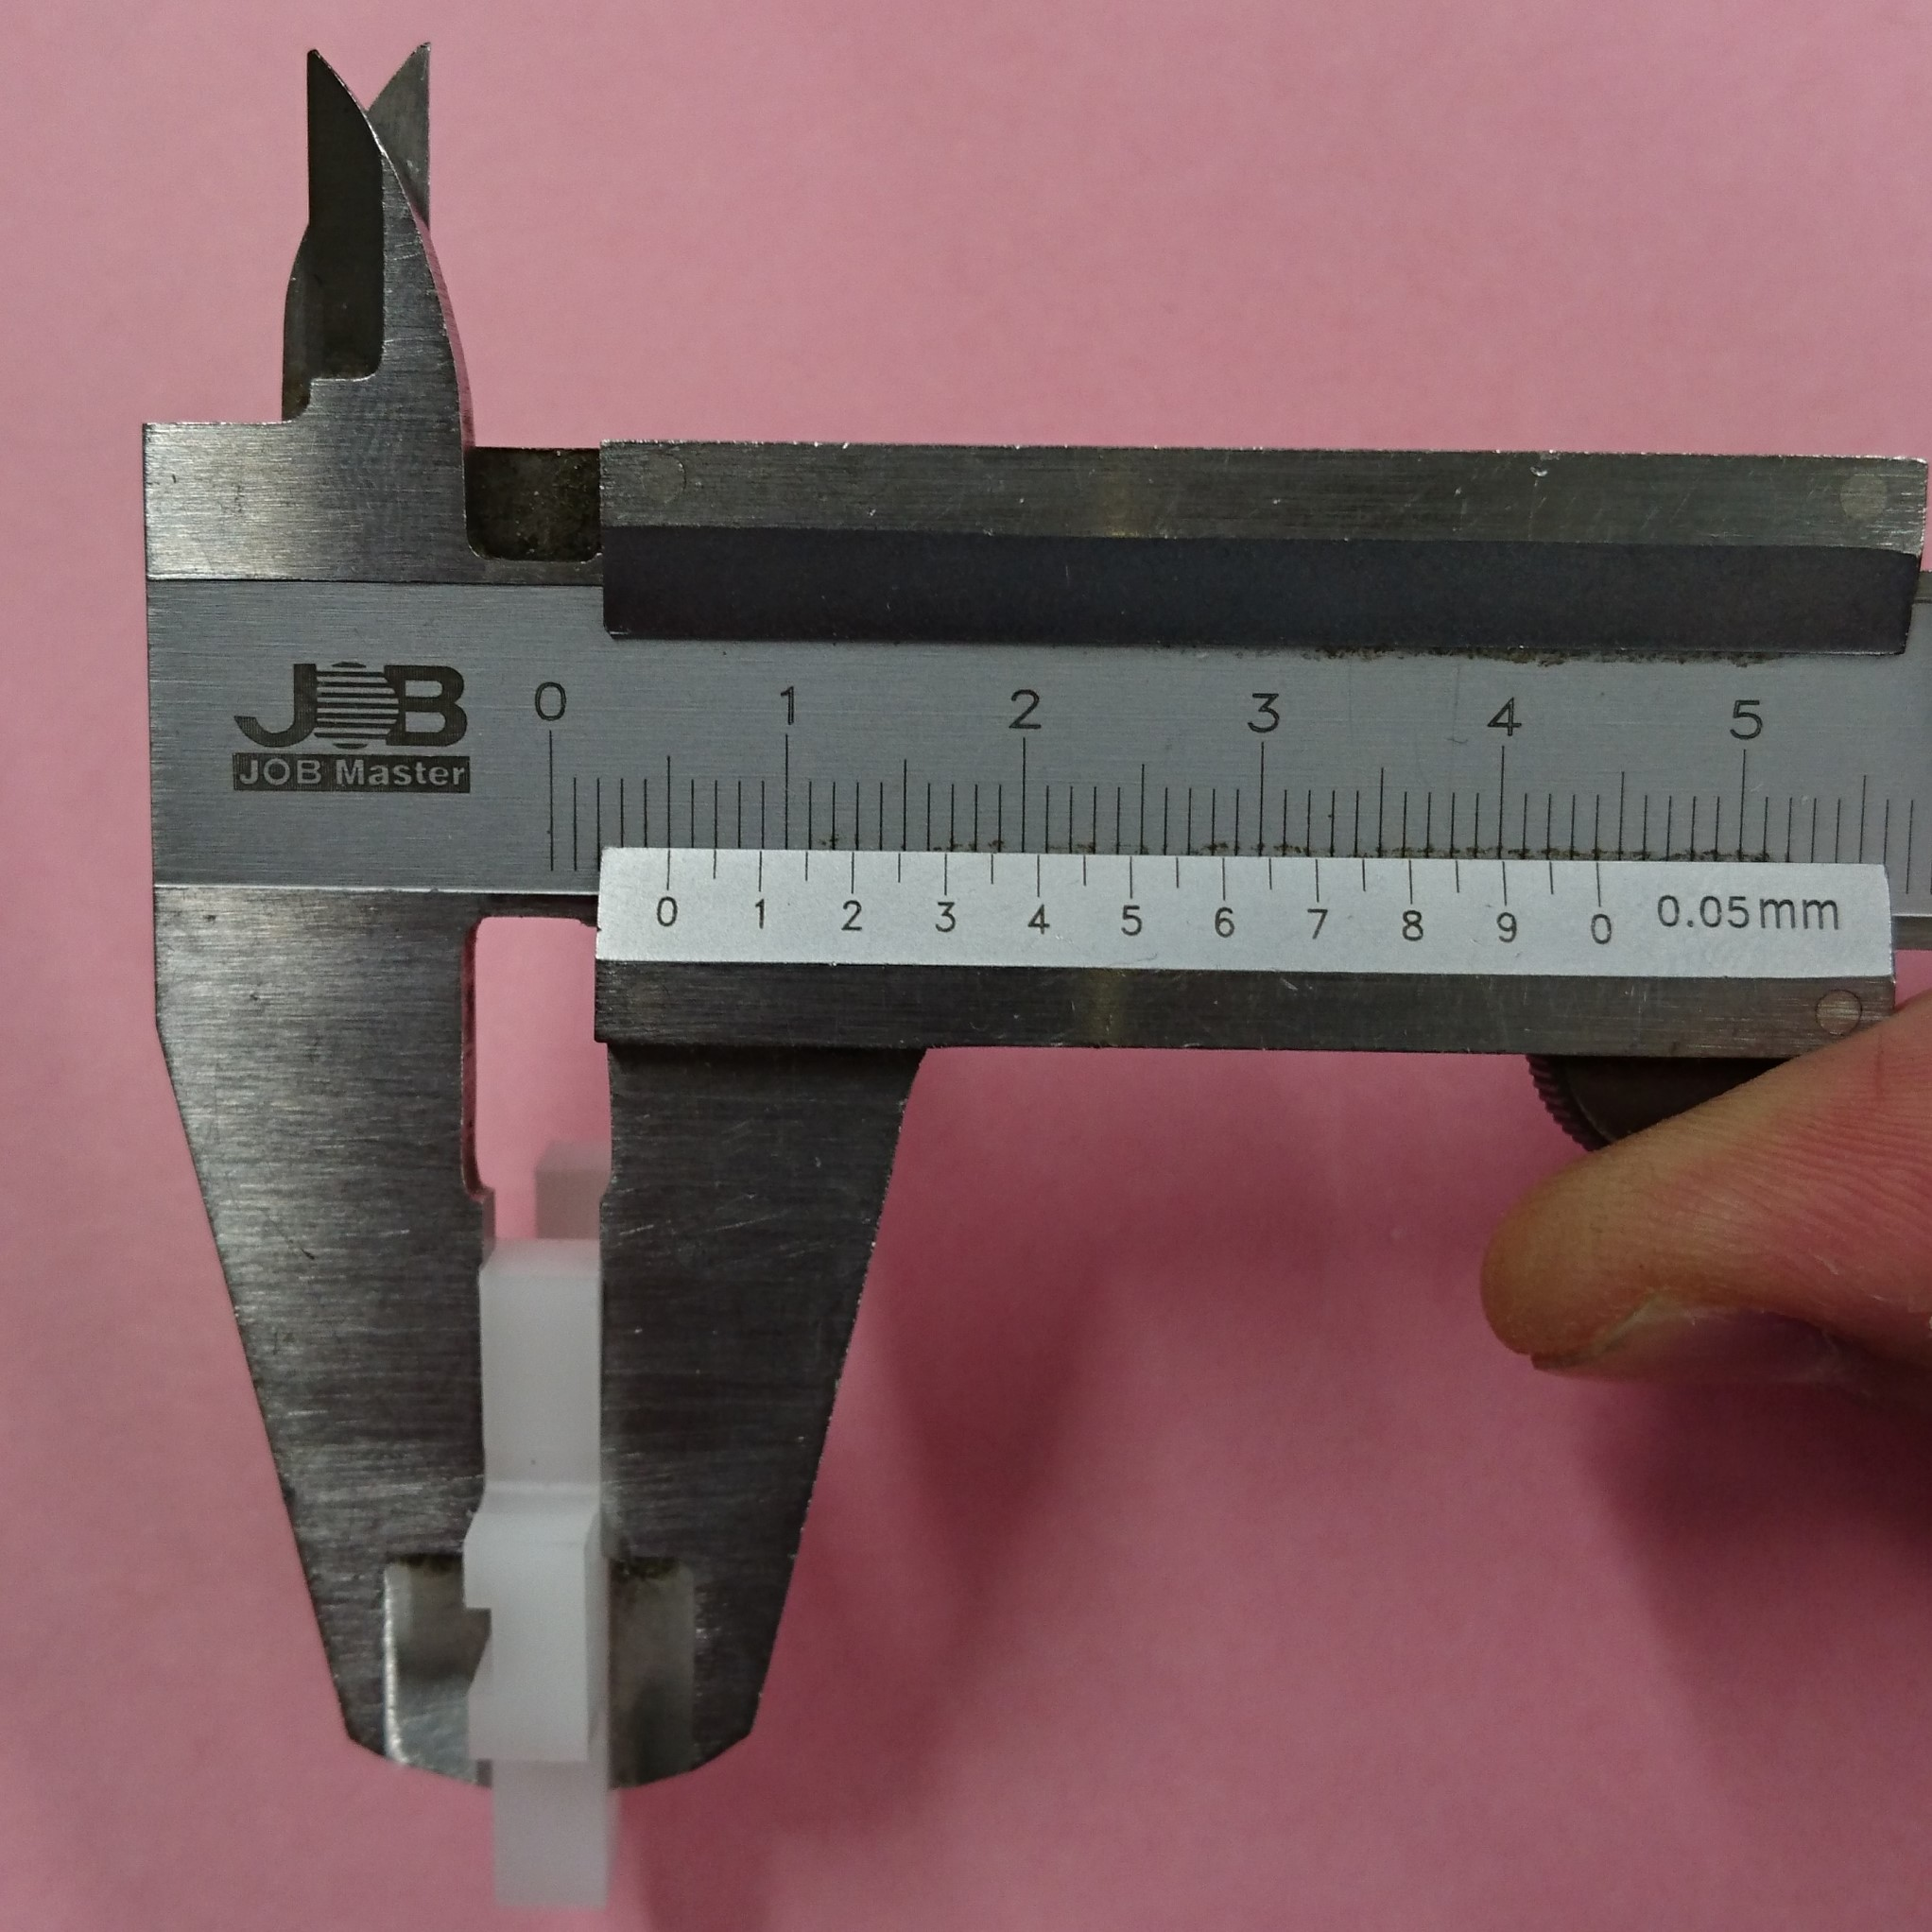
\includegraphics[width=\columnwidth]{thickness.jpg}
    \end{minipage}
    \caption{厚み計測\label{thickness}}
  \end{center}
\end{figure*}

%%  画像*5 バリ取りカッター、バリの画像、仕上げ後の画像(通常、アイソメ)、厚み精度 baritori.jpg parts_bari.jpg parts.jpg parts_isome.jpg thickness.jpg

\clearpage
\section{小ネタ}
\subsection{削り残しを防ぐコツ}
基本的には、計測した厚みを元にして、丁度削り切れるような深さで切削を行うのですが、それでもほんの少し削り残しが出てしまうことがあります。POMなどのバリが取りやすい材料であればさほど問題にならないのですが、6ナイロンなど削り残しを除去するのが難しい材料を使う際にはなるべく避けたい問題です。かと言って切削する深さを考えなしに大きくするとCNCの捨板を傷つけてしまいます。こういった場合、材料を固定するのに使う両面テープの存在を利用することで、削り残しを防ぐことができます。具体的には、両面テープの厚み分の0.2mm程度を削る深さに加えることで、両面テープが少し削れる程度の深さでの加工になるため、普通にやるより削り残しが出にくくなります。注意点としては、通常より両面テープのカスがエンドミルに残りやすいので、加工後の清掃は入念に行いましょう。\\

\subsection{部品を複製する}
Cut2Dのベクトル操作を使うことで、簡単に部品を複数作ることができます。まず通常通りに経路を作ります。その後、鏡面部品を作りたい部分のベクトルを選択・コピー(ctrl-c)・貼り付け(ctrl-v)をすることで同じ場所に二重にベクトルが生成されます。貼り付けをした直後だと二重になったベクトルのうち片方の組だけが選択されているため、その状態でベクトルの移動を行います。移動量は部品のサイズと、加工に必要なエンドミルの太さ以上のマージンを考慮して決めて下さい。これを縦横に繰り返すと、一つの部品のベクトルの組から、多くの部品のベクトルの組を作ることができます。この状態だと切削経路まではコピーされないので、それぞれの経路の編集に戻ってそれぞれの組の中で同じベクトルを選んだ上で再度経路の計算を行って下さい。\\

\subsection{鏡面対象部品を作る}
基本的には部品の複製と同じですが、移動した後にベクトルのセットをまるごと反転することで鏡面のベクトルを作ることができます。作った後は複製と同様に経路ごとに対応するベクトル選択し、再度計算を行ってください。この時気をつける部分として、反転する基準をベクトルの中心にすることです。基準を誤ると、反転した後に元の部品のベクトルと被ってしまう場合があるので気をつけて下さい。\\

\clearpage
\chapter*{最後に}
以上でCNC切削加工入門は終わりです。近年3Dプリンタやレーザー加工機の普及によって、ハードウェアの製作のハードルが下がっていると感じています。それらを用いることで、確かに簡単に素早く部品の製作・試作を行うことができます。しかし、作ることができる部品の剛性や精度を考えると、用途によってはCNCでの切削加工が必要になると思います。また、CNC切削加工の場合でも、CADに付属しているCAMの中には、モデルを入れるだけで自動で加工経路を設計してくれるものもあります。ですが、自分でベクトルを作るところから経路の設計まで一通り行えると、より高い自由度で切削加工を行うこと可能です。このような思いから、CNC加工を広めたいと感じて、CNC切削加工入門を書くに至りました。こうして文章化してみることでtips的な細かい注意点の多さを再確認して、改めてハードウェア製作の新規参入のハードルの高さを感じました。あくまでこの入門は入門でしかないので、ぜひ皆さんも実際にCNC加工を経験して。楽しんで学んでみて下さい。\\時代は切削!

\begin{comment}
\bibliographystyle{junsrt}
\bibliography{p-report}
\end{comment}

\begin{thebibliography}{99} %参考文献

\bibitem{pla_properties}プラスチック物性値の比較 \url{http://www.kda1969.com/study/study_pla_compare.html}

\bibitem{alminium_properties}アルミの物性値 \url{http://www.alumitech.co.jp/html/download5.html}

\end{thebibliography}

\end{document}

\begin{comment}
  \begin{figure}[tbh]
    \begin{center}
      \begin{minipage}{0.3\columnwidth}
        \includegraphics[width=\columnwidth]{hozon.png}
        \caption{eps図の参考例}
      \end{minipage}
      \hspace{0.15\columnwidth}
      \begin{minipage}{0.3\columnwidth}
        \includegraphics[width=\columnwidth]{plane.png}
        \caption{jpg図の参考例}
      \end{minipage}
      \label{figure:nowprinting}
    \end{center}
  \end{figure}
\end{comment}
